\documentclass[type=doctor]{thuthesis}
% 选项:
%   type=[bachelor|master|doctor|postdoctor], % 必选
%   secret,                                   % 可选
%   pifootnote,                               % 可选(建议打开)
%   openany|openright,                        % 可选,基本不用
%   arial,                                    % 可选,基本不用
%   arialtoc,                                 % 可选,基本不用
%   arialtitle                                % 可选,基本不用

% 所有其它可能用到的包都统一放到这里了,可以根据自己的实际添加或者删除。
\usepackage{thuthesis}
\usepackage[lined,boxed,commentsnumbered,resetcount,algochapter]{algorithm2e}
% 定义所有的图片文件在 figures 子目录下
\graphicspath{{figures/}}

% 可以在这里修改配置文件中的定义。导言区可以使用中文。
% \def\myname{薛瑞尼}

\begin{document}

%%% 封面部分
\frontmatter
\thusetup{
  %******************************
  % 注意:
  %   1. 配置里面不要出现空行
  %   2. 不需要的配置信息可以删除
  %******************************
  %
  %=====
  % 秘级
  %=====
  %secretlevel={绝密},
  %secretyear={2100},
  %
  %=========
  % 中文信息
  %=========
  ctitle={视频与图像中的背景减除技术研究},
  cdegree={工学博士},
  cdepartment={计算机科学与技术系},
  cmajor={计算机科学与技术},
  cauthor={孙丰},
  csupervisor={秦开怀教授},
  % 日期自动使用当前时间,若需指定按如下方式修改:
  % cdate={超新星纪元},
  %
  % 博士后专有部分
  %cfirstdiscipline={计算机科学与技术},
  %cseconddiscipline={系统结构},
  %postdoctordate={2009年7月——2011年7月},
  %id={编号}, % 可以留空: id={},
  udc={UDC}, % 可以留空
  catalognumber={分类号}, % 可以留空
  %
  %=========
  % 英文信息
  %=========
  etitle={Research on background subtraction techniques for images and videos},
  % 这块比较复杂,需要分情况讨论:
  % 1. 学术型硕士
  %    edegree:必须为Master of Arts或Master of Science(注意大小写)
  %             “哲学、文学、历史学、法学、教育学、艺术学门类,公共管理学科
  %              填写Master of Arts,其它填写Master of Science”
  %    emajor:“获得一级学科授权的学科填写一级学科名称,其它填写二级学科名称”
  % 2. 专业型硕士
  %    edegree:“填写专业学位英文名称全称”
  %    emajor:“工程硕士填写工程领域,其它专业学位不填写此项”
  % 3. 学术型博士
  %    edegree:Doctor of Philosophy(注意大小写)
  %    emajor:“获得一级学科授权的学科填写一级学科名称,其它填写二级学科名称”
  % 4. 专业型博士
  %    edegree:“填写专业学位英文名称全称”
  %    emajor:不填写此项
  edegree={Doctor of Philosophy},
  emajor={Computer Science and Technology},
  eauthor={Sun Feng},
  esupervisor={Professor Qin Kaihuai},
  %eassosupervisor={Chen Wenguang},
  % 日期自动生成,若需指定按如下方式修改:
  % edate={December, 2005}
  %
  % 关键词用“英文逗号”分割
  ckeywords={背景减除, 移动相机, 视频, 图像显著性, 图像填充},
  ekeywords={background subtraction, moving camera, video, image saliency, image inpainting}
}

% 定义中英文摘要和关键字
\begin{cabstract}
  
  
\end{cabstract}

% 如果习惯关键字跟在摘要文字后面,可以用直接命令来设置,如下:
% \ckeywords{\TeX, \LaTeX, CJK, 模板, 论文}

\begin{eabstract}
   An abstract of a dissertation is a summary and extraction of research work
   and contributions. Included in an abstract should be description of research
   topic and research objective, brief introduction to methodology and research
   process, and summarization of conclusion and contributions of the
   research. An abstract should be characterized by independence and clarity and
   carry identical information with the dissertation. It should be such that the
   general idea and major contributions of the dissertation are conveyed without
   reading the dissertation.

   An abstract should be concise and to the point. It is a misunderstanding to
   make an abstract an outline of the dissertation and words ``the first
   chapter'', ``the second chapter'' and the like should be avoided in the
   abstract.

   Key words are terms used in a dissertation for indexing, reflecting core
   information of the dissertation. An abstract may contain a maximum of 5 key
   words, with semi-colons used in between to separate one another.
\end{eabstract}

% \ekeywords{\TeX, \LaTeX, CJK, template, thesis}

% 如果使用授权说明扫描页,将可选参数中指定为扫描得到的 PDF 文件名,例如:
% \makecover[scan-auth.pdf]
\makecover

%% 目录
\tableofcontents

%% 符号对照表



%%% 正文部分
\mainmatter
\chapter{引言}
\label{cha:intro}

\section{研究意义}
\label{sec:first}
视觉是人类感知世界最直接和重要的方法之一,光线通过眼睛、视网膜、大脑等器官的处理,最终形成我们所感知的图像~\cite{GonzalezDIP}。随着科技的发展,数码相机、摄像机等的出现使得数字图像和视频成为了人们日常生活中最常见的数字媒体之一。特别是随着近年来智能手机、移动互联网、社交网络的飞速发展和普及,人们随时随地都可以将眼前所见拍摄成图像或视频,并通过网络分享给自己在世界各地的亲朋好友。这些海量的数字图像和视频信息的处理已经成为计算机科学等领域重要的研究内容。当前,图像和视频处理已经从传统的基于像素的处理,例如图像去噪、图像增强、图像压缩等,逐步转移到基于内容的处理,例如基于内容的编辑、基于内容的检索等~\cite{CMM12THU}。根据经验,我们在观察图像或视频时,一般会将注意力集中在某些感兴趣区域,例如,在观看电影时我们的视觉注意力主要集中在主要角色身上。生物学家和心理学家通过研究和实验证实,人类的视觉系统只对图像的某些局部进行处理,而对其余部分几乎完全忽略~\cite{treisman1980a,Koch1985Shifts}。一般将人类视觉系统感兴趣的这类对象称为前景对象或显著性对象(saliency objects);相反,图像中的另外一部分则称为背景。背景减除,或前景检测,是指将图像或视频中背景部分去除,从而使前景对象和背景对象分离的一种技术。例如,在图~\ref{fig:1}中,~\ref{fig:subfig1}中为输入图像,~\ref{fig:subfig2}中为背景减除技术提取的前景对象,其中用白色表示前景区域,黑色表示背景区域。\par
\begin{figure}[ht]
  \centering%
  \subcaptionbox{输入图像\label{fig:subfig1}} %标题的长度,超过则会换行,如下一个小图。
    {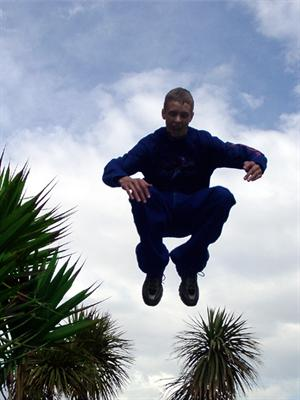
\includegraphics[width=0.3\textwidth]{ch1/0_0_818.jpg}}%
 \hspace{1em}%
  \subcaptionbox{背景减除结果,白色为前景,黑色为背景\label{fig:subfig2}}
      {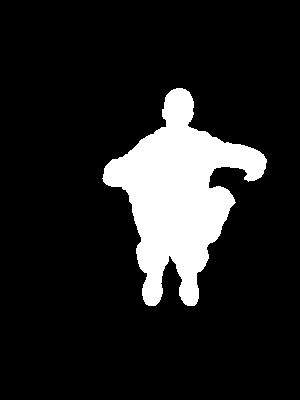
\includegraphics[width=0.3\textwidth]{ch1/0_0_818.png}}
  \caption{图像背景减除示例}
  \label{fig:1}
\end{figure}
在由连续的图像序列组成的视频中,根据相对运动情况,一般将相对相机运动的对象视为前景,其它相对静止的部分则归为背景。当拍摄视频的摄像机保持固定时,分离前景和背景只需定位那些存在运动的对象。而当拍摄视频的摄像机也存在旋转、平移、缩放等运动时,会造成视频中所有像素都产生运动。这时,只能通过区分相机引起的运动和前景产生的运动来区分前景和背景。例如,在图~\ref{fig:videoBS}中,图~\ref{fig:frame1}、~\ref{fig:frame10}分别为视频中第1帧和第10帧图像,图~\ref{fig:frame1Fg}、~\ref{fig:frame10Fg}中为对应图像帧的背景减除结果,其中用白色表示前景区域,黑色表示背景区域。
\begin{figure}[ht]
  \centering%
  \subcaptionbox{视频第1帧图像\label{fig:frame1}}[3cm] %标题的长度,超过则会换行,如下一个小图。
    {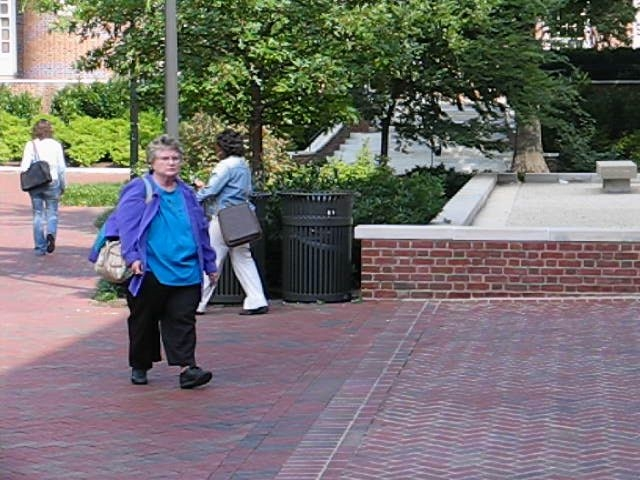
\includegraphics[width=0.22\textwidth]{ch1/in000001.jpg}}%
  \hspace{1em}%
  \subcaptionbox{视频第10帧图像\label{fig:frame10}}
      {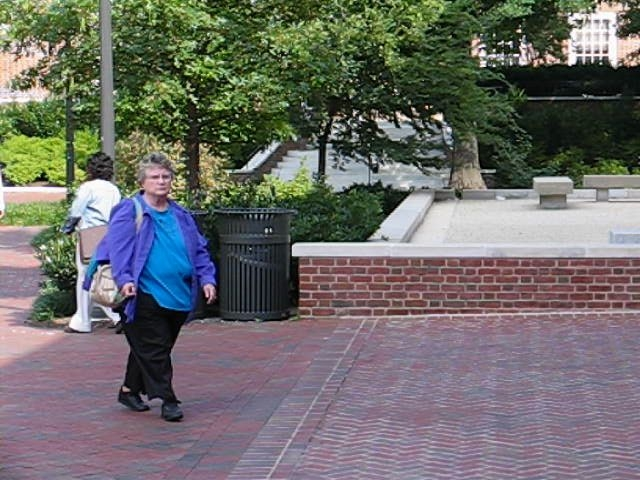
\includegraphics[width=0.22\textwidth]{ch1/in000010.jpg}}
  \hspace{1em}%
  \subcaptionbox{第1帧图像前景\label{fig:frame1Fg}}
      {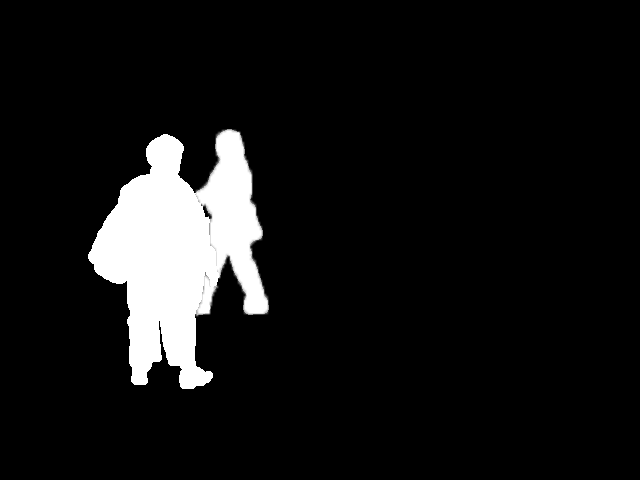
\includegraphics[width=0.22\textwidth]{ch1/gt000001.png}}
   \hspace{1em}%
   \subcaptionbox{第10帧图像前景\label{fig:frame10Fg}}
    {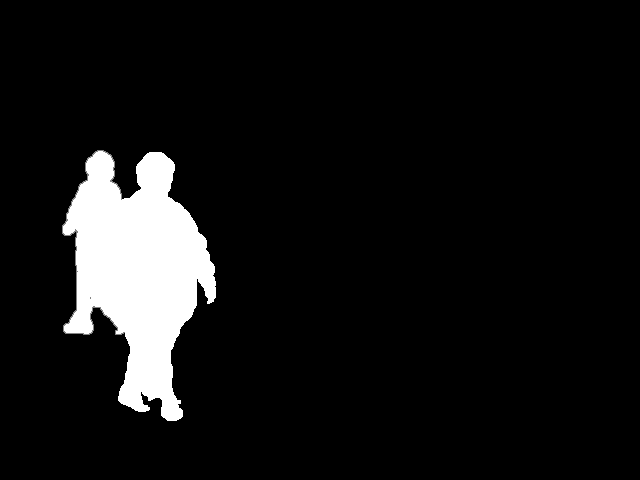
\includegraphics[width=0.22\textwidth]{ch1/gt000010.png}}

  \caption{视频背景减除示例}
  \label{fig:videoBS}
\end{figure}
\par

背景减除通常作为计算机尝试分析并理解图像的第一步,是内容感知的图像处理~\cite{Avidan:2007}、视频监控~\cite{Collins1998A}、目标识别与跟踪~\cite{YilmazTracking}、基于深度的绘制(depth image based rendering,DIBR)~\cite{Fehn03a3d-tv}等应用领域中重要的预处理步骤。例如,在内容感知的图像缩放应用中,为了在对图像进行缩放编辑时保持前景对象的比例,首先需要对图像进行显著性分析,确定显著性对象的位置。在DIBR中,为了处理因遮挡而产生的空洞,需要利用图像中的其它像素对空洞进行填充。因为被遮挡的部分基本上是背景区域,因此如果误将前景像素填充到空洞中,会造成鬼影、闪烁等问题,影响绘制视频的质量。利用背景减除技术对视频进行预处理,可以有效避免将前景像素用于空洞填充,提高视频的绘制质量。\par

综上所述,背景减除技术是计算机视觉研究中一个非常热门的课题。提高背景减除技术的准确度和速度对于众多相关应用具有十分重要的意义。
\section{研究现状}
\label{sec:second}
\subsection{图像显著性分析}
\label{sec:imageSaliency}
图像显著性区域检测的目标是在计算机上实现像人眼一样快速判断图像中显著性区域的能力,通过这种技术提取的图像显著性区域可以广泛用于目标识别,图像编辑以及图像检索等应用。Itti等人~\cite{itti}提出了最早的显著性检测模型,该模型结合了认知心理学,神经科学和计算机科学的理论和方法。基于人类注意力自底向上,关注中心与四周差异的特点,该模型预测人眼观察图像时的焦点,能得到一系列离散的圆点形状的显著性区域预测结果,并不能得到显著性对象的准确边界。随后,显著性检测研究的热点集中在如何获得显著性对象的准确边界,并把它们从图像中分割出来。在这种情况下,显著性检测可以被看作是一个图像分割问题,目标是把图像分割为显著的和非显著的两个部分。如图~\ref{fig:SaliencyOverview}所示,图~\ref{fig:saliencyInput}为输入图像,图~\ref{fig:ITRes}为文献~\inlinecite{itti}所提出算法得到的结果,图~\ref{fig:RCRes}为文献~\inlinecite{ChengPAMI}所提出算法得到的结果,图~\ref{fig:GT}为人工标记的正确结果。

\begin{figure}[ht]
  \centering%
  \begin{subfigure}{0.2\textwidth}
    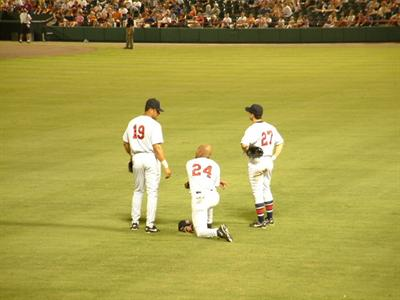
\includegraphics[width=\textwidth]{ch1/0_5_5108.jpg}
    \caption{输入图像}
    \label{fig:saliencyInput}
  \end{subfigure}%
  \hspace{0.1in}%
  \begin{subfigure}{0.2\textwidth}
    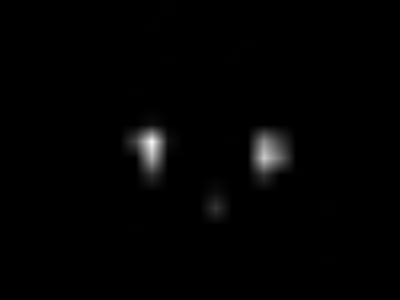
\includegraphics[width=\textwidth]{ch1/0_5_5108_IT.png}
    \caption{~\inlinecite{itti}的结果}
    \label{fig:ITRes}
  \end{subfigure}
  \hspace{0.05in}%
   \begin{subfigure}{0.2\textwidth}
    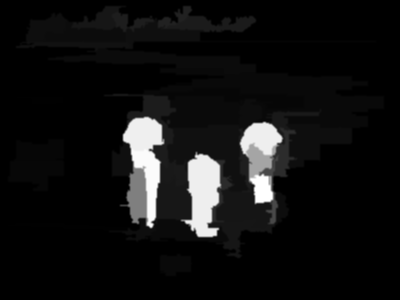
\includegraphics[width=\textwidth]{ch1/0_5_5108_RC.png}
    \caption{~\inlinecite{ChengPAMI}的结果}
    \label{fig:RCRes}
  \end{subfigure}
  \hspace{0.05in}%
   \begin{subfigure}{0.2\textwidth}
    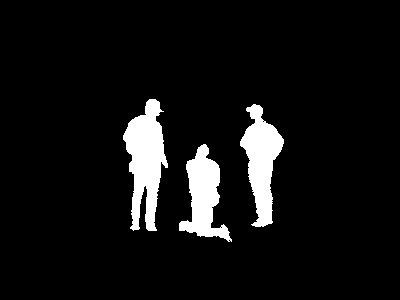
\includegraphics[width=\textwidth]{ch1/0_5_5108.png}
    \caption{正确结果}
    \label{fig:GT}
  \end{subfigure}
  \hspace{0.05in}%
  \caption{显著性分析算法比较}
  \label{fig:SaliencyOverview}
\end{figure}



最近几年以来,显著性区域检测问题一直是计算机视觉等相关研究领域的研究热点~\cite{saliencySurvey}。研究人员提出了一系列新算法,使得显著性对象的准确度以及算法的速度有了显著提高。一般认为,在定位显著性对象时一般依靠内部和外部两种线索\cite{saliencySurvey},其中内部线索来自于待处理图像自身,而外部线索可能来自于用户交互或来自于其它图像的信息。从应用和效率的角度来说,基于内部线索的算法更加贴近实际应用。早期,研究人员关注的内部线索主要是显著性对象的独特性(uniqueness)。这种特性具体表现为,显著性对象与其相邻区域存在较大差异。Achanta等人~\cite{frequenyTuned}提出利用高斯滤波后图像与图像平均颜色差距来计算每个像素的显著性值,图像中像素$x$的显著性指标被定义为:
$$s(x)={\parallel I_{\mu }-I_{\omega}(x)\parallel}^{2}$$
,其中$I_{\mu }$是图像所有像素的平均颜色,$I_{\omega}$是经过高斯滤波后的图像。文献~\inlinecite{patchUniquenss}中提出了一种基于分块独特性(patch uniqueness)的算法,该算法认为图像中那些与最其相似分块的距离大的分块具有较高的显著性水平,并在计算分块显著性时考虑了分块之间的空间距离。Margolin等人~\cite{whatmakes}提出利用分块与图像平均分块的距离来定义分块显著性值,他们认为显著性水平高的分块在高维空间中的分布要更为分散,因此利用分块与平均分块在主元分量方向的距离来定义分块的显著性。\par
然而,基于分块的算法容易使得具有高对比度的图像边缘获得很高的显著性值,而有时这些边缘部分并不是真正的显著性区域。另外,受分块大小参数的影响,这类算法那最终所得的显著性对象的边缘并不准确。基于以上原因,越来越多的显著性分析算法引入了基于区域的分析方法。与基于分块的方法不同,基于区域的方法首先利用区域分割算法对图像进行分割得到若干个齐次的小区域。相比于基于分块以及基于像素的算法, 区域分割处理可以保持对象边界,同时利用区域颜色直方图可以更准确的对区域内的颜色对比度进行量化。另外,以区域为单位计算大大降低了运算量。Cheng等人~\cite{ChengPAMI}提出了一种基于区域对比度的显著性检测算法。该算法首先利用基于图的分割算法~\cite{graphseg}将图像分给为$N$个齐次区域$\{r_{i}\}_{i=1}^{N}$。区域$r_{i}$的显著性值定义为:
$$s(r_{i})=\sum_{j=1}^{N}\omega_{ij}D_{r}(r_{i},r_{j})$$
其中$D_{r}(r_{i},r_{j})$是区域$r_{i},r_{j}$之间的颜色直方图距离,$\omega_{ij}$是区域之间的空间相关性度量。
Perazzi等人~\cite{saliencyFilter}提出利用欧几里得距离来计算$D_{r}(r_{i},r_{j})$,并将显著性计算转换为高斯滤波过程。与文献~\inlinecite{ChengPAMI}中一样,该算法首先将图像进行抽象化(abstraction),去掉不必要的细节部分,将图像分为若干个齐次区域。与~\inlinecite{ChengPAMI}中所用的基于图的图像区域分割算法~\cite{graphseg}不同,文献~\inlinecite{saliencyFilter}中使用了边界保持性更好的超像素分割算法~\cite{SLIC}。除了对比度等独特性线索之外,常用的显著性线索还包括中心线索,即图像中显著性对象一般位于图像中靠近中心的位置。此外,文献~\inlinecite{ufo}中提出显著性区域应该在相机的焦点之上,而利用图像中边缘的模糊性可以对图像区域是否在图像焦点上进行量化,综合考虑区域的对比度,和区域中包含对象的可能性(objectness),得到最终显著性结果。\par
与上述基于显著性线索的算法不同,另一类算法从相反的方向考虑问题,利用背景线索来定位背景,最终剩下显著性前景。与显著性对象不同,图像中背景区域具有连续性强;与周围区域相似度高;靠近图像边缘;背景区域之间对比度低等特点。文献~\cite{geodesicDistance}中提出一种基于背景线索的显著性检测算法,该方法利用背景部分像素容易连接到图像边界的特点,利用图像区域距离图像边界的测地线距离(geodesic distance)来评估其显著性。文献~\inlinecite{backgroundPrior}中利用了图像边界大部分是背景这一假设,首先对图像边界区域进行对比度分析,从中获得背景区域主要颜色的线索,之后利用这一线索进行对比度分析获得显著性前景结果。\par
Hou等人~\cite{SpectralSaliency}提出基于频域分析的显著性区域检测算法, 该算法虽然有处理速度的优势但在准确性上相比于基于空间域的方法还有较大差距。 Huang等人~\cite{Huang2011}提出一种内容感知的随机化图像显著性检测算法,该算法利用多个层次下的粗糙显著性检测结果合成最终结果, 同时选择性的对显著性结果中不可靠的区域进行更新以优化最终结果。此外, 文献~\inlinecite{DISC,NIPS2014_5547}中均提出基于机器学习的图像显著性检测算法。

\subsection{图像填充技术}
\label{sec:imageInpainting}
在图像显著性分析中,一般把显著性对象称为前景对象。这些对象是人眼在观察图像时主要关注的对象。然而在另一种应用场景下,前景和背景需要根据用户的定义来确定,这时原本属于前景的对象可能被用户定义为背景。例如,如图\ref{fig:inpainting}所示,最左边图像中的三棵树原本是前景对象。但因为用户希望获得一幅只有海面和白云的图像而被标记为背景,如图\ref{fig:Inpaint_subfig2}所示,用户希望去掉所标记的对象后得到\ref{fig:Inpaint_subfig3}中的结果。

\begin{figure}[ht]
  \centering%
  \subcaptionbox{输入图像\label{fig:Inpaint_subfig1}}[3cm] %标题的长度,超过则会换行,如下一个小图。
    {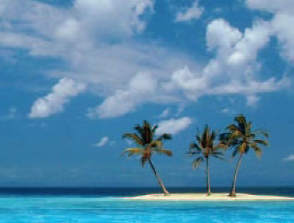
\includegraphics[height=3cm]{ch1/inpaint1.png}}%
  \hspace{4em}%
  \subcaptionbox{红色区域为用户标注的背景\label{fig:Inpaint_subfig2}}
     {
\includegraphics[height=3cm]{ch1/inpaint2.png}}
  \hspace{1em}%
   \subcaptionbox{用户期望的结果\label{fig:Inpaint_subfig3}}
    {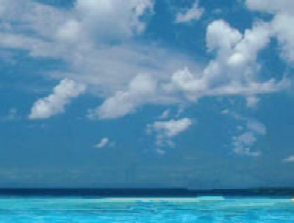
\includegraphics[height=3cm]{ch1/inpaint3.png}}
  \caption{图像修复示例~\cite{Criminisi04regionfilling}}
  \label{fig:inpainting}
\end{figure}

这一应用类型一般被称为图像填充(image inpainting),或图像补全(image completion)。其中用户标注的区域为需要填充的部分,这部分区域根据用户需求而定。在很多情况下包含显著性对象。在填充时,希望能最大限度的保持图像的结构连续性和完整性,使得填充后图像在视觉上没有被修补过的痕迹。图像填充技术在图像编辑、图像去噪、图像编码领域、基于图像的渲染等应用中发挥着重要作用。在我们的日常生活中也经常遇到这样的应用场景,例如在游人如织的旅游景点拍照时会将旁边的路人拍进了画面,这时希望在不破坏原图像的条件下将其从画面中删除;去掉老照片上发黄的部分或者数据丢失后照片中的瑕疵;去掉照片上的文字标题等。\par
假设图像 \emph{I} 中包含未知或缺失部分\(\Omega\) 以及已知区域 \(\overline{\Omega}\),图像填充的目标是利用\(\overline{\Omega}\)中的信息,或者借助来自原图像外部的信息来填充\(\Omega\) 区域。从广义上说,可以把图像填充问题看做是一种特殊的背景减除,需要填充的\(\Omega\)相当于不需要的背景区域,而减除操作相当于用特定像素来填充这些背景区域。图像填充算法大致可以分为两类~\cite{inpaintingSurvey},基于散射(diffusion)的方法~\cite{Bertalmio:2000}和基于样本(examplar)的方法~\cite{Criminisi04regionfilling}。前者利用图像连续和平滑性(smoothness priors)的特点,通过建立参数化的偏微分方程模型方法将已知区域的信息扩散到未知区域。这类方法容易使填充后的图像产生模糊,在缺失区域较大的情况下尤为明显。另一类基于样本的方法则以小图像块为样本,不断将已知区域的结构以及纹理信息传递到位置区域。这类方法不会产生模糊问题,且对图像结构的连续性处理较好。基于样本的方法假设缺失部分的信息可以通过与之最匹配的样本来填充。如图~\ref{fig:examplar}所示,黑色区域为待填充的未知区域\(\Omega\),$\psi_{p}$为以\(\Omega\)的边缘上一点$p$为中心的方块,$\psi_{q}$为\(\overline{\Omega}\)中与$\psi_{p}$最匹配的分块。
\begin{figure}[ht]
  \centering%
      {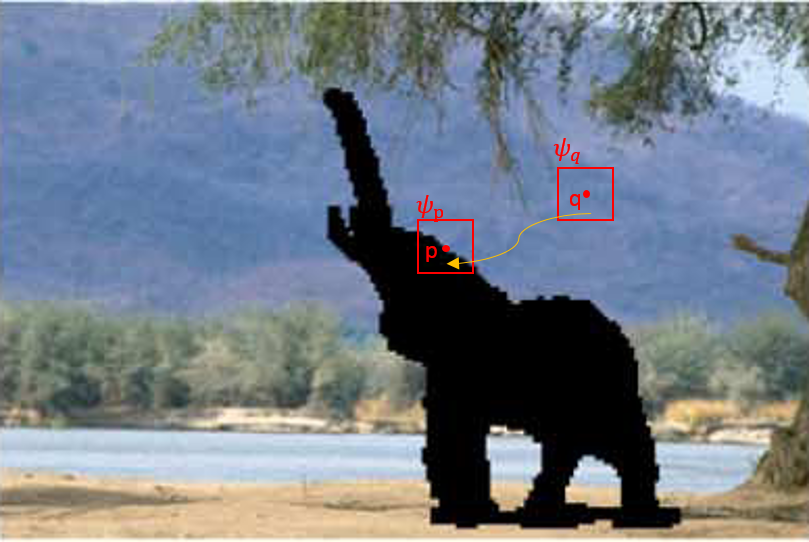
\includegraphics[height=6cm]{ch1/examplar.png}}
  \caption{基于样本的图像修复}
  \label{fig:examplar}
\end{figure}
Efros等人~\cite{Efros}利用$\psi_{q}$的中心点像素来填充$p$,即:
$$Output(p)=Value(q),p\in \Omega, q\in \overline{\Omega},q=\arg \min d(\psi_{p},\psi_{q})$$
,利用分块之间的均方差之和(sum of squared differences,SSD)来计算分块之间的距离,评估分块之间的相似性:
$$d(\psi_{p},\psi_{q})=\sum_{i}^{N}\sum_{j}^{N}\left \| \psi_{p}(i,j)-\psi_{q}(i,j) \right \|^{2}$$
其中$N$为样本的长度和宽度。Criminisi等人~\cite{Criminisi04regionfilling}对Efros等人的算法进行了改进,首先利用未知区域边缘曲线的辐射度方向(isophoto direction)与法向量的夹角来确定分块的填充优先级,使得包含结构信息的分块优先填充,从而保证纹理信息能从已知区域扩散到未知区域;其次,利用最佳匹配块中的对应像素来填充对应未知分块中的像素,比Efros等人的算法效率更高。但是,文献~\inlinecite{Criminisi04regionfilling}提出的算法在一些困难情况下无法恢复未知区域的连续结构信息。文献~\inlinecite{userInpainting}提出了一种用户交互式的基于结构传播的图像补全算法,该方法利用用户输入的一些曲线或者直线把未知区域分为纹理区域和结构区域。对于这两种区域,分别利用不同的策略来恢复纹理信息或结构信息。Xu等人~\cite{Xu:2010}提出另一种基于分块稀疏性(patch sparsity)的图像填充算法,该算法利用分块的稀疏性来确定填充顺序。与之前的方法不同,Xu等人所提算法中并不是只用一个最佳匹配块来对未知区域进行填充,而是利用多个分块的组合来填充未知分块。虽然Xu等人所提算法在填充效果上优于文献~\inlinecite{Criminisi04regionfilling}的算法并且接近基于用户交互的算法~\cite{userInpainting},但是其计算复杂度过高,需要几分钟来处理一张普通大小的图像。Barnes等人~\cite{Barnes:2009}提出一种非常快的随机匹配算法,称为PatchMatch。该方法利用图像的空间相关性,以随机迭代的方式寻找图像的最佳匹配块,并用其进行图像填充。该算法被应用在Adobe公司的Photoshop软件的内容感知填充功能中。虽然PatchMatch算法的速度非常快,处理纹理区域效果好,但是却无法处理包含大块未知结构信息的情况。在这两类算法之外,还有一些算法利用了输入图像之外的信息来进行填充。华淼等提出通过网络检索在互联网或联机数据库中根据输入图像以及所缺失信息进行搜索,寻找合适图像完成输入图像未知区域的填充~\cite{huamiao}。


\subsection{静止相机情况下的视频背景减除}
\label{sec:staticCamera}
在早期的视频背景减除技术研究中,一般假设摄像机是静止的。基于这一假设,通过建立不包含前景对象的背景模型,并将其它图像帧与背景模型进行比较得到前景。
在图~\ref{fig:2}中是一个典型的视频背景减除算法流程图。假设输入视频帧的前$N$帧图像中不包含前景对象,利用这些图像初始化背景模型,在$t$时刻得到的背景模型为$B(t)$。
在下一时刻,将视频图像帧$I(t)$与$B(t)$进行匹配,其中匹配成功的像素标记为背景,反之则为前景。最后利用所得前景结果和当前帧信息对$B(t)$进行更新,得到$B(t+1)$。
由此可见,背景模型的对算法的准确度至关重要。

\begin{figure}[htb]
  \centering%
  {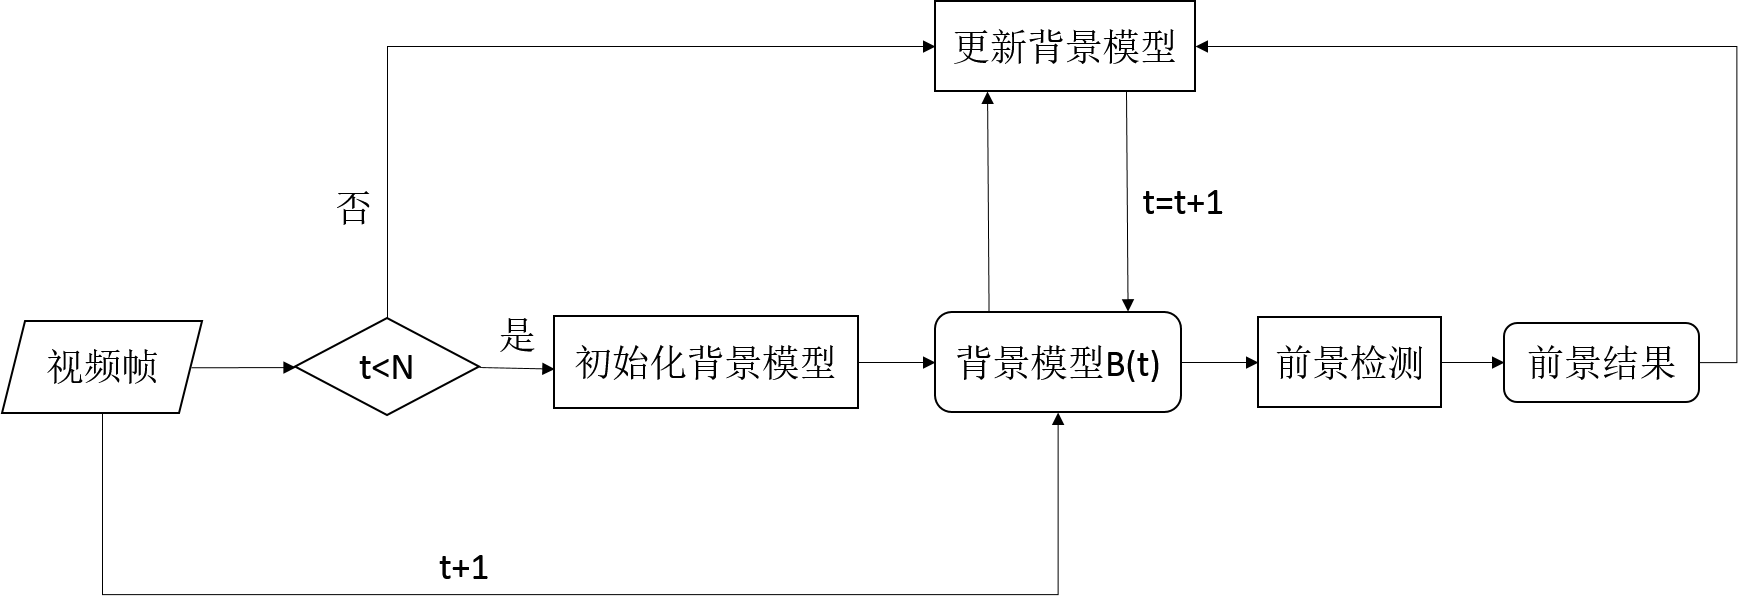
\includegraphics[width=0.9\textwidth]{ch1/bsflowchart.png}}%
  \caption{背景减除流程图~\cite{BouwmansOverview}}
  \label{fig:2}
\end{figure}
最简单的背景模型可以通过对输入视频帧进行平均~\cite{LeeAverage}或者中值滤波~\cite{MF}的方式得到,然而这种方法对噪声的处理并不理想。为了解决这一问题,研究人员提出了一系列基于统计模型的背景建模方法。Chien等人~\cite{Chien2002Efficient}提出了一种基于图像注册背景建模方法,利用一幅图像作为背景模型。该方法首先对视频相邻帧进行
差分操作,并对结果进行二值化得到掩码图像$M$。$M$中值为0的像素为相邻帧图像亮度变化在门限之内的像素,这些像素属于背景的概率较大;然后,观察连续多帧图像产生的$M$,若$M$中某像素长期为0,则其被判为可靠背景像素,并将当期图像帧此位置的像素值复制到背景图像中;最后,将后续的视频帧与背景图像进行差分操作得到前景结果,并对背景图像进行更新。该方法
简单高效,但其依赖固定门限,且仅以一幅图像作为背景模型,无法处理亮度变化大以及包含动态背景的视频。假设视频中像素的亮度值的变化可以用高斯模型来建模,Wren等人~\cite{Wren}提出了单高斯背景模型,随后Kim等人~\cite{kim2007robust}对其进行了改进。然而,这种单高斯模型无法处理像被风吹动的树叶、流动的水等这种动态背景。Stauffer~\cite{stauffer1999adaptive}等人提出了基于自适应混合高斯模型的背景模型建模方法,利用多个高斯模型对背景像素进行建模。相比于单高斯模型,混合高斯模型处理亮度变化大及包含动态背景的视频时效果虽然得到了显著提升,但其前景误检率仍较高。Barnich等人~ \cite{Barnich2011ViBe}提出了一种名为ViBe的无参数采样模型背景建模方法。该方法通过$N$个背景图像色彩空间采样值来描述背景模型:
$$M(x)=\{v_{1},v_{2},...,v_{N}\}$$ \par
如图~\ref{fig:vibe}所示,为了区分某像素$v(x)$是否属于背景,ViBe算法在二维欧几里德色彩空间内计算以$v(x)$为中心的圆形范围$S_{R}(v(x))$内的采样值与背景模型$M(x)$交集的数量,当$\#\{S_{R}(v(x))\bigcap\{v_{1},v_{2},...,v_{N}\} \}$大于或等于某门限值时像素$v(x)$被判为背景,否则为前景。

\begin{figure}[ht]
  \centering%
  {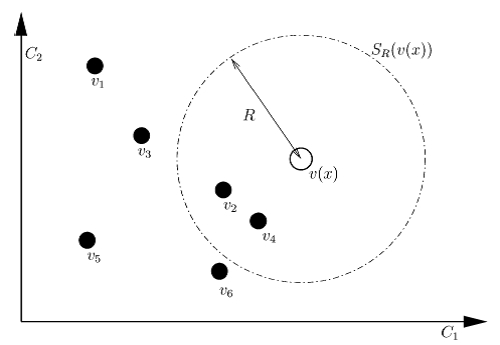
\includegraphics[width=0.5\textwidth]{ch1/vibe.png}}%
  \caption{ViBe算法示意图~\cite{Barnich2011ViBe}}
  \label{fig:vibe}
\end{figure} \par


在背景模型初始化过程中,ViBe算法在第一帧图像中按照均匀分布随机的从像素邻域中选取像素值:${M}^{0}(x)=\{v^{0}(y\mid y\in N_{G}(x))\}$。虽然这种初始化方法可能会将在第一帧中的移动对象设为背景从而产生鬼影现象,但是随着模型的更新,这种现象会逐渐消失。ViBe算法使用一种新的保守的背景更新策略,与之前的更新方法不同的是该算法从背景像素点的历史值中收集样本值,不断更新随机时间序列,当新的样本值加入到背景模型中时随机地将历史样本值丢弃。具体的说,ViBe定义背景模型中的采样值在更新时保留的概率为:
$$P(t,t+dt)={\left(\frac{N-1}{N} \right)}^{(t+dt)-t}$$ \par
另外,为了降低背景更新的频率,ViBe算法还采用时间采样的方式来延长模型的生命周期。若某像素被分类为背景,则以一定的概率(如$\frac{1}{16}$)用该像素的值去更新模型。为了保证空间一致性并使被前景区域覆盖的背景点被更新,在更新时将当前帧$x$点处的像素值去更新在空间八邻域上的邻近像素点的背景模型。ViBe算法简单,鲁棒性强,但也存在一些缺陷:
 \begin{itemize}
\item 当运动目标与背景对比度小的情况下,ViBe 算法提取的目标轮廓存在缺陷,导致目标轮廓不封闭,容易产生轮廓内部孔洞现象;
\item 监控场景下的运动目标有阴影时算法检测出的前景存在阴影现象。
\end{itemize}
\par
Droogenbroeck等人对ViBe算法进行了改进~\cite{vibe},主要修改了距离函数和判别门限,区分更新蒙版和输出蒙版并对其进行了滤波,在更新背景模型时对某些像素进行了限制,当视频中摄像机有抖动时,增大更新系数并检查像素的闪烁。修改后的ViBe算法比原算法普适性更强,并且在检测正确率等方面也有所提高。Hofmann等人~\cite{pbas}提出了一种带反馈的基于像素的自适应视频背景分割算法, 称为PBAS。该方法和ViBe算法一样都是无参数方法。该方法的基本思想和ViBe类似,主要的区别在于PBAS通过自适应的方法对模型更新相关参数进行自适应调整。这种自适应调整通过闭环反馈的方式实现,背景判决门限和更新率等参数可以在处理过程中通过反馈的方式自适应调整,调整后的参数可以获得更好的性能。在测试中PBAS方法的检测准确率等性能参数超过了ViBe,而且同样可以实现实时检测。在近期的一项工作中 \cite{subsenseTIP}, 作者提出了一种更加有效的反馈式模型更新背景建模方法,SuBSENSE. 该算法的准确度在CD.Net 2012~\cite{CDNet2012} 和CD.Net 2014~\cite{CD2014}数据集中均优于其它算法。因为同样是基于采样模型,该算法效率高且易于实现。\par
与上述算法不同,Lin等人~\cite{lin2002a}引入了更复杂的统计模型支持向量机模型(support vector machine,SVM),利用SVM分类器对所有训练视频帧像素进行分类并添加到背景模型,直到不出现新的背景像素时停止模型初始化。SVM所用的特征包括光流信息和图像帧间的差分图像。此外,研究人员还提出了基于子空间学习~\cite{uray2007incremental}和基于频域分析~\cite{Gao2009}的背景模型。文献~\inlinecite{BouwmansOverview}对这些算法进行了总结和分类。

\subsection{移动相机情况下的视频背景减除}
\label{sec:movingCamera}
随着移动计算平台(如智能手机、手持摄像机、智能机器人等)的快速发展, 移动相机视频越来越普及, 针对移动相机拍摄视频的背景减除技术越来越重要。 与静止相机的情况相比, 移动相机下的背景减除要困难很多, 因为相机的运动使得视频中前景和背景像素都会产生运动, 区分相机产生的运动和前景自身运动是待解决的主要难题。另外,如果能利用图像帧准确估算出相机运动,并进行运动补偿,就可以将移动相机情况转换为固定相机情况处理。\par
 文献~\inlinecite{iccv2009}提出一种基于点轨迹的背景减除算法, 根据背景点轨迹矩阵的秩等于3的特点~\cite{Tomasi_1992}, 以滑动窗口的方式利用随机抽样一致(random sample consensus, RANSAC) 算法~\cite{Ransac} 在点轨迹矩阵中检测背景点。 同样基于点轨迹并考虑前景像素的集中性, 文献~\cite{Cui2012}提出一种基于点轨迹矩阵分解的算法。Berger等~\cite{SubspaceTracking}提出一种基于线性子空间跟踪的背景建模算法, 与基于点轨迹的同类算法相比, 该算法的背景检测更准确, 且处理速度更快, 但其处理一帧图像仍需要1.6秒。 另外, 由于这类算法是基于点轨迹的, 而计算视频中稠密像素的长期轨迹是一项十分耗时且困难的工作, 即使在GPU 加速的情况下也需要几秒的时间处理一帧图像~\cite{ECCV10DensePonintTrajectories}。\par

为了处理相机的运动, 另一类算法引入了稠密光流。 文献~\cite{kwak2011Generalized}提出一种基于贝叶斯滤波的背景减除算法框架, 该算法需要视频第一帧的准确前景作为输入, 并在随后的视频帧中利用稠密光流信息进行可靠跟踪; 这种算法需要人工交互来生成第一帧的准确前景, 不适用于在线处理, 且无法处理长时间且包含复杂相机运动的视频. 文献~\cite{gbsuperpixel}提出另外一种基于稠密光流的移动相机视频背景减除新算法, 通过建立基于超像素的背景模型, 并基于二进制置信传播技术通过多次迭代获得像素级精度的前景; 虽然该算法的准确度要优于其他算法, 但其处理一帧大小为$300\times200$的视频帧需要6秒。\par
文献~\cite{5.8s}提出一种实时的移动相机下视频背景减除算法, 由于该算法利用基于固定特征点跟踪的相机运动估算算法和简化的双模高斯背景模型, 使得算法复杂度低速度较快, 并可以实现实时处理。但文献~\cite{5.8s}没有给出该算法前景检测准确度的定量分析。 本文通过实验发现, 文献~\cite{5.8s}算法的前景检测准确度较低, 特别是在相机移动幅度较大的情况下, 无法适应前景检测准确率要求较高的应用。\par
在估算相机运动,一般采用单应性矩阵或基础矩阵来描述相机运动情况。 文献~\inlinecite{Multitransform}中提出了一种多变换模型的方法来处理相机运动。该算法根据相邻帧图像的几何变换情况,自适应地从单应性矩阵模型和基础矩阵模型中选择一个模型。当选择单应性矩阵时,根据特征点的运动情况估算全局单应性矩阵并用于相机运动补偿,而当选择基础模型使用时,基于最小均方误差的方式在一系列单应性矩阵中选择一个误差最小的单应性矩阵作为全局参数补偿相机运动。\par
崔智高等~\cite{czg}提出一种基于多组单应约束和马尔可夫随机场(Markov random field,MRF)的移动目标检测算法, 通过轨迹分离和像素标记2个阶段实现移动相机拍摄视频中运动目标的检测; 该算法检测前景的准确度较高, 但由于算法是基于点轨迹的, 同样存在算法计算量大的问题。



\section{研究目标与主要贡献}
\label{sec:contents}
快速识别图像和视频中的显著性前景,将前景对象从背景中分离出来是人类的视觉系统与生俱来的能力。然而,在计算机上实现人眼的这种能力却十分困难。对于图像显著性检测,主要的困难在于:
 \begin{itemize}
     \item 前景的多样性和不确定性。相比于人脸识别、指纹识别等应用,显著性检测的目标并不固定。在不同的场景下,前景对象的定义存在不确定性,例如,在一张汽车广告画中汽车是前景对象,然而同样是汽车, 在车模的特写照片中却成为背景;
	\item 复杂背景情况。当图像中的背景较复杂时,会使得背景部分的像素也具有对比度高、独特性明显等性质,而这些指标常用于检测显著性对象,这时容易将背景误识别为前景,造成误检率高。
\end{itemize}
当前视频背景减除面临的主要困难主要有:
\begin{itemize}
	\item 噪声干扰。在环境噪声的干扰下,我们得到的视频图像中可能包含一些噪声,这些噪声会对前景提取的准确度造成重要的影响。例如在雨雪天气或者夜间拍摄的视频中,存在亮度不足,雨雪对前景判别产生干扰等问题;
    \item 动态背景,在视频背景减除中,我们在判别前景和背景时一般假设背景区域的像素是静止,而运动的像素则属于前景。然而,在实际应用中,这一假设并不总是成立。例如视频中被风吹动摇摆的树叶,喷泉,以及流动的水面等。这些对象虽然是运动的,但实际却属于背景;
    \item 相机的运动,在早期的视频背景减除技术研究中,一般假设相机是静止的。然而,随着移动计算平台,例如手机、手持摄像机、智能机器人等的出现,移动相机拍摄视频中的背景减除技术研究越来越重要。在移动相机拍摄的视频中,区分相机运动和前景运动是一项困难的工作。
  \end{itemize}

\par
在图像填充技术方面,主要的困难在于保持图像结构信息的连续性,此外当前效果较好的算法速度较慢,处理一张普通大小的图像可能要几分钟时间,很难满足人们在线处理的应用需求。针对上述这些问题,本论文围绕图像和视频中的背景减除技术展开研究,主要研究目标是提出更加高效且准确的方法来提取图像和视频中的显著性前景。本论文主要研究内容为图像显著性检测、图像填充以及针对移动相机拍摄视频的背景减除,主要贡献总结如下:
 \begin{itemize}
    \item 将图像显著性区域检测问题视为图像分割问题,提出以显著性引导的区域合并的方式将图像分为显著性区域(前景)和背景两个区域。在合并过程中采用了与主流算法相反的策略,即不再尝试定位显著性区域,而是利用背景线索来估计背景区域,并不断将显著性差的非前景区域合并到背景区域。利用背景连续性强、靠近图像边缘、相对前景对比度低等背景线索,首先将图像进行超像素分割,随后在区域显著分析的引导下,不断将显著性最差的区域合并到背景区域,而不是尝试将显著性区域合并到一起。 最后,利用合并过程中得到的多个候选显著性区域加权得到最终的显著性区域结果。在国际上两个公开的数据库中的共计2000张图像上对本文所提出的算法进行了测试,实验结果验证了算法的有效性。在主要由自然图片组成,较为困难的ECSSD~\cite{ECSSD}测试集中,本文算法得到的F-Mearsure以及平均绝对误差(mean absolute error,MAE)均优于其它同类算法。此外,本文的算法简单直观,且效率高、易于实现;
    \item 针对现有的基于样本的图像填充算法容易造成结构信息不连续且计算量大的问题,提出了一种基于样本的两阶段快速图像填充算法,以两次填充的方式将结构以及纹理信息填充到图像中的未知区域中。该算法首先利用离散小波变换(discrete wavelet transform, DWT)获取低分辨率的输入图像,并利用基于样本的填充算法进行填充。由于高频细节部分被DWT过滤,在低分辨率填充后的图像中纹理部分区域可以获得较好的结果,但是在包含边缘的局部还存在着结构不连续的情况。针对这些问题,在这些区域中再进行第二次填充。在填充过程中,提出基于梯度结构张量的填充优先级计算方法以及基于加权SSD的最佳匹配块标准以提高填充后图像的结构和纹理连续性。为了提高效率,提出了以分块结构性测试和动态搜索窗口的方式寻找最佳匹配分块,减少冗余计算。本文提出的填充算法可以得到与当前先进算法相近的结果,但是在处理速度上却有明显优势;
    \item 提出了一种基于无参数模型的快速视频背景减除算法。该算法利用两种线索来有效检测移动相机拍摄视频中的前景对象。第一种线索基于色彩空间采样模型,通过引入最相似变形(as-similar-as-possible warping, ASAPW)方法来准确估算相机运动并进行补偿,然后将变形后的图像与背景模型进行匹配得到一张粗略的前景分割图像;第二种线索来基于前景引起的运动与相机引起的运动的差异。利用稀疏光流和相机运动的差异获取背景种子点,提出一种基于超像素种子点的区域增长算法,将稀疏的背景种子点扩散到整张图像,获得另一张粗略的前景图;最后为了融合两种线索的结果并考虑时间上的相关性,提出了一种基于超像素的MRF优化框架,将两种线索得到的粗略前景以及上一帧图像所得的前景结果值一起输入优化方法,最后通过图割算法求解得到最终结果;
    \item 提出了一种针对移动相机的实时背景减除算法。该算法假设视频中大部分区域是背景, 前景只占相对较小部分。考虑背景像素的连续性, 提出了一种基于超像素的区域增长算法对图像进行预处理。 为了估算相机运动, 提出了一种基于相对光流的特征点筛选算法, 筛选出属于背景的特征点, 并利用这些特征点以分块的方式估算相机的运动。 最后通过比较这些超像素的光流与所估算的相机运动的一致性来确定最终的前景。该算法简单直接, 不需要建立任何背景模型, 利用GPU和CPU的混合编程可以实现实时处理。 大量实验证明该算法的前景检测准确度远高于同类实时算法。
  \end{itemize}
\section{本文的组织结构}
本文第一章为引言,介绍了论文的研究背景和意义,并对国内外相关工作进行了综述,最后介绍了本文的研究内容以及主要贡献。第二章研究图像显著性检测问题,介绍了本文提出的基于区域合并的图像显著性检测算法,第三章中介绍本文提出的基于样本的快速图像填充算法,第四章和第五章研究移动相机情况下的视频背景减除问题,第四章中介绍了本文提出的基于无参数模型的快速背景减除算法,第五章介绍了本文提出的另一种简单有效的实时背景减除算法。第六章对全文进行了总结和展望。
\label{sec:hierarchy} 


\chapter{基于区域合并的图像显著性检测}
\label{ch2:SGRM}
本章提出了一种显著性引导的图像区域合并算法,用于图像显著性区域检测。算法的目标是直接通过区域合并的方式逐渐将图像从初始状态下的多个区域合并为显著性对象和背景2个区域。为实现这一目标,在不同的阶段采用不同的合并策略。首先利用超像素分割方法将图像分为若干初始区域。在第一阶段,仅合并相似且相邻的区域,使得属于同一对象的像素合并到同一区域;随后进行第二阶段合并,处理上述过程中产生的空洞以及因遮挡造成的属于同一对象的区域不相邻的情况;在第三阶段合并时,以区域显著分析结果为引导,不断将显著性最差的区域合并到背景区域,而不是尝试将显著性区域合并到一起;最后,利用合并过程中得到的多个候选显著性区域加权得到最终的显著性区域结果。为了验证算法的有效性,在2个国际上公开的测试集ASD~\cite{Achanta08}和ECSSD~\cite{ECSSD}上测试了本章所提算法,并与其它同类算法进行了对比。实验结果证明了本章所提算法的有效性,特别是在难度更大的ECSSD数据集~\cite{ECSSD}中,本章算法的准确度要优于其它同类算法。
\section{研究背景}
\label{sec:background}
图像显著性区域检测是近年来计算机视觉和图像处理领域的研究热点之一~\cite{saliencySurvey}。该技术的目标是快速定位图像中显著性对象,可以广泛应用于目标识别,基于内容的图像编辑以及图像检索等应用中。早期的显著性检测算法~\cite{itti}依据视觉感知理论,采用自底向上方法预测人眼观察图像时的焦点(fixation),最终得到一系列离散的圆点形状的显著性区域预测结果。然而,这类方法效率和准确度均较低,且无法得到显著性对象的准确边界,实际应用范围受限。随后,为了实现提前显著性对象的准确边界,研究人员提出了一系列数据驱动,自底向上的显著性区域检测算法~\cite{Achanta08,ChengPAMI,ufo,Yan2014Hierarchical},大大提高了显著性对象检测精度以及计算速度。目前这类算法均可以较为准确的提取自然图像中包含的显著性对象,实现显著性对象与背景的分离。\par
据文献~\inlinecite{Borji2015Salient}报道,在这些算法中,基于图像区域的算法性能更出色。基于区域的显著性检测算法首先用超像素~\cite{SLIC}、基于图的图像分割算法~\cite{graphseg}等图像分割方法将图像分为若干个小区域,随后以区域为单位进行显著性计算。由于在区域分割时考虑了像素在色彩以及空间域的连续性,分割后的区域内像素具有很好的齐次性,且大部分区域之间的边界与图像边缘吻合。 相比于基于像素的算法, 区域分割处理在保持显著性对象边界的同时,可以利用区域颜色直方图更准确的对区域内的颜色对比度进行量化。另外,以区域为单位计算大大降低了运算量。\par
当前大部分已有的图像显著性检测算法的出发点均是根据显著性区域的特点,例如对比度高~\cite{ChengPAMI}、处在相机焦点上~\cite{ufo}等,定义区域显著性模型以计算每个像素的显著性水平。然而,自然图像中可能包含各种类型的显著性对象,单纯用这些显著性对象的线索仍然无法处理所有情况。如图~\ref{fig:saliencyCom}所示,(a)为输入图像,(b)、(c)、(d)分别为CHS算法~\cite{Yan2014Hierarchical}、RC算法~\cite{ChengPAMI},和本章算法的结果,(e)为正确结果。图~\ref{fig:saliencyCom}表明,当输入图像中对象和背景的色彩分布较为接近(图~\ref{fig:saliencyCom}中第一行和第二行),或者背景复杂度较高(第三行)时RC和CHS算法均无法有效检测出显著性对象。
\begin{figure}[htb]
  \centering%
      {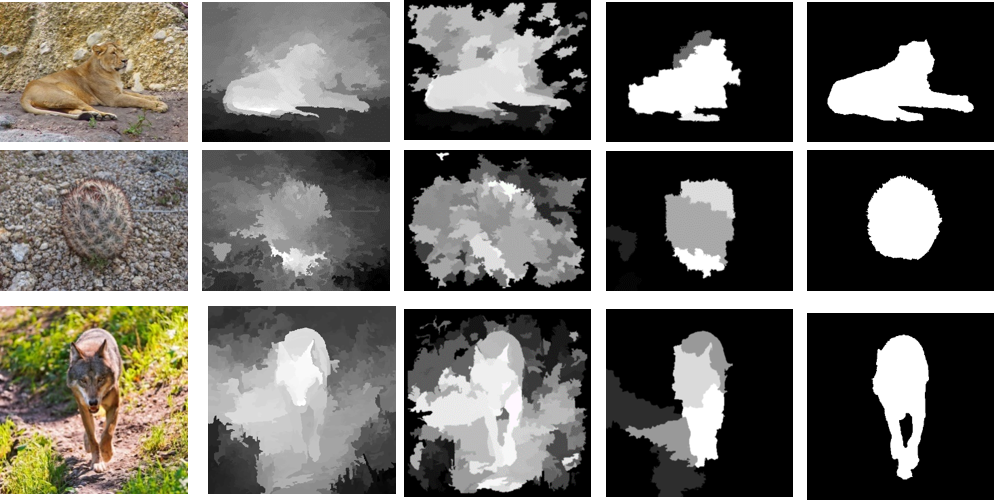
\includegraphics[width=0.9\textwidth]{ch2/ch02fig1.png}}\\
(a)\quad\quad\quad\quad\quad
(b)\quad\quad\quad\quad\quad\quad
(c)\quad\quad\quad\quad\quad\quad
(d)\quad\quad\quad\quad\quad
(e)
  \caption{显著性检测结果对比}
  \label{fig:saliencyCom}
\end{figure}

\par
为了解决这一问题,本章将显著性区域检测问题视为图像分割问题,以显著性引导的区域合并的方式将图像分为显著性区域(前景)和背景两个区域。在合并过程中采用了与主流基于区域的图像显著性检测算法~\cite{Achanta08,ChengPAMI,ufo,Yan2014Hierarchical}相反的策略,即不再尝试定位显著性区域,而是利用背景线索来估计背景区域,并不断将显著性差的非前景区域合并到背景区域。根据观察,大部分自然图像中的背景部分的像素具有连续性强的特点~\cite{huamiao},例如室外拍摄图像中的天空,地面等背景区域。此外,图像的边缘部分应该大部分都是背景~\cite{backgroundPrior}。如果不断将图像中相似的小区域进行合并,背景部分像素应该更容易合并到一起,并且将包含更多的图像边缘。观察图~\ref{fig:saliencyCom}中输入图像的背景部分,如第一行图像中的地面以及狮子身后的山、第二行图像中的石块地面、以及第三行图像中的草地,虽然这些背景部分色彩分布与前景接近或者具有较高的复杂度,其仍然具有这种较强的连续性。在区域合并时本文没有尝试将显著性区域合并到一起,而是利用背景区域线索,首先将图像进行超像素分割,随后在区域显著分析的引导下不断将显著性最差的区域合并到背景区域。最后,利用合并过程中得到的多个候选显著性区域加权得到最终的显著性区域结果。将本章算法在两个公开的数据库ASD~\cite{Achanta08}和ECSSD~\cite{ECSSD}中的共计2000张图像中进行了测试并与其它算法进行了对比,实验结果验证了本章所提算法的有效性。在较为困难的ECSSD测试集中,本章算法得到的F-Mearsure以及平均绝对误差(MAE)均优于其它参与比较的相关算法。

\section{相关工作}
\label{sec:relatedWorks}
\subsection{图像显著性区域检测}
\label{sec:SaliencyDetection}
对比度(contrast)强是显著性对象区别于背景的重要性质,Cheng等人~\cite{ChengPAMI}提出利用全局对比度的方法计算图像中每个颜色的显著性水平。由于色彩空间巨大,为了提高效率,Cheng等人提出以量化的方式提取图像中的主要颜色并依据此建立直方图,计算每个颜色的显著性值。为了进一步提高算法的准确度,Cheng等人~\cite{ChengPAMI}提出了一种基于区域对比度的方法,先用基于图的图像分割方法将图像分为若干齐次区域,考虑区域的空间相关性,利用区域对比度来检测显著性区域,得到了比全局对比度更好的效果。Perazzi等人~\cite{saliencyFilter}提出基于高维高斯滤波的显著性滤波算法(saliency filters)。该算法首先对待处理图像进行抽象化,去掉冗余细节信息。随后在CIELab色彩空间中通过局部及全局对比度来计算色彩独特性,利用高维高斯滤波的方式结合色彩的空间分布情况计算最终的显著性检测结果。Jiang等人~\cite{ufo}指出,作为主要目标显著性对象应该在成像时处于相机焦点之上,利用图像中边缘的模糊程度可以对图像区域是否在成像时处于相机的焦点上进行量化,最后综合考虑图像区域对比度、是否在相机焦点上以及区域中包含对象的可能性(objectness)三方面线索计算最终的结果。Li等人~\cite{DSR}提出一种基于重建误差的显著性检测算法, DSR。 该算法首先利用超像素提取图像的边界, 计算每个区域的稠密及稀疏重建误差; 随后利用$K$-means算法对重建误差信息进行聚类, 最后通过多尺度重建误差集成和偏向对象的高斯模型优化得到像素级的显著性结果。 Jiang等人\cite{MC}提出一种基于图像图模型上的吸收马尔可夫链的算法, 该方法结合了显著性对象的独特性和背景区域的空间分布特点等线索, 利用马尔可夫链模型中各节点至边界吸收节点的吸收时间来评估像素的显著性。 为了处理自然图像中的复杂结构,Yan等人~\cite{ECSSD}提出了一种多尺度层次化的显著性区域检测算法,称为CHS。该方法将图像在不同尺度上进行分割,得到多个层次的区域显著性线索,并将这些多层次的线索进行加权得到最终结果。本章所提出的方法与CHS算法有类似之处,均采用了图像区域合并的方法得到多个图像分割结果。但不同之处在于本章提出的区域合并方法在合并过程中的不同阶段使用不同的合并策略,而CHS算法使用同样的分层策略得到固定数量的层次。并且,本章使用背景线索进行区域显著性分析,与上述基于显著性对象线索的算法均不同。\par
Wei等人~\cite{geodesicDistance}提出了一种基于背景线索的显著性检测算法,该方法利用背景部分像素容易连接到图像边界的特点,利用图像区域距离图像边界的测地线距离(geodesic distance)来评估其显著性。文献~\inlinecite{backgroundPrior}中利用了图像边界大部分是背景这一假设,先对图像边界区域进行对比度分析,从中获得背景区域主要颜色的线索;随后利用这一线索利用基于~\inlinecite{ChengPAMI}的算法进行对比度分析获得显著性前景结果。本章算法基于类似的背景线索,但是本章所提算法通过显著性引导的区域合并的方式进行显著性检测,这与文献~\inlinecite{geodesicDistance,backgroundPrior}有较大差别。\par
与基于区域的算法不同, Wang等人~\cite{PISA}提出一种基于像素的显著性检测算法, PISA。 该算法主要利用图像全局范围内的颜色和结构对比度及其在图像空间域中的分布情况等线索,以滤波的方式将多种线索合成得到图像中每个像素的显著性值。虽然PISA算法的准确度与本章算法较为接近,但是由于PISA是基于像素的算法,本章算法与之相比在速度上有明显优势。

\subsection{图像区域合并}
\label{sec:regionMerging}
图像区域合并是指根据图像区域之间的相似性,逐渐将相似的区域合并在一起的过程,常用于图像分割等应用中。Richard~\cite{Richard2004Statistical}提出了一种基于统计的区域合并的图像分割算法,利用图像统计特性确定需要合并的区域以及合并的顺序。在算法的初始阶段,每个像素表示一个区域,以相邻区域间颜色的差值的升序进行排序。在合并过程中,按此顺序将区域间颜色差距在门限之内的区域进行合并,直到剩余的区域数量达到合并要求。文献~\inlinecite{Xiao2015Complexity}提出了一种复杂度自适应的图像区域距离以衡量图像区域的相似性,并以之为基础评估区域间的相似性。在合并时,优先合并相似区域。在区域合并完成后,根据区域中包含边缘信息的情况来评估区域中包含对象的可能性(objectness)。文献~\inlinecite{SelectiveSearch}中提出了一种基于贪心算法的图像区域合并方法,该方法不断合并所有邻居区域中最接近的两个区域,直到将整幅图像合并为一个区域。上述区域合并方法作为预处理方法用于对象识别和显著性区域检测算法中取得了不错的效果。但上述方法均在区域合并过程中均始终采用同一策略,没有考虑到区域合并过程中不同阶段的不同特点,容易将属于前景对象的像素合并到背景区域。\par
如图~\ref{fig:rm}所示,图~\ref{fig:sub:img}为输入图像,其中水面上划船的人为显著性前景对象。分别利用文献~\inlinecite{Richard2004Statistical}、~\inlinecite{Xiao2015Complexity}所提出的图像区域合并算法对输入图像进行分割,得到结果如图~\ref{fig:sub:srm}和图~\ref{fig:sub:cadm}所示。输入图像被分为9个区域,分别用不同的随机颜色表示。从图中可以看出,当分割进行到此阶段时,文献~\inlinecite{Richard2004Statistical}、~\inlinecite{Xiao2015Complexity}算法会将前景对象合并到背景区域中。其中图~\ref{fig:sub:cadm}中结果更为明显,划船人被分割到多个区域中。出现这种情况的主要原因是在合并过程中随着区域逐渐扩大区域间的相似度越来越高,如果在合并时只考虑区域间在色彩及空间上的相似度则很容易将属于前景区域与属于背景的区域合并到一起。另外,前景对象一般具有连续和紧凑的特点,即属于前景的对象的空间分布较为集中。如果在合并时仅允许相邻的区域进行合并~\cite{SelectiveSearch}可以在一定程度上防止前景区域合并到背景区域。但是考虑到前景对象对背景的遮挡,又会使得背景区域无法合并到一起。例如,图 ~\ref{fig:sub:img}中输入图像中背景部分的树林,由于前景对象的遮挡,这部分区域不再联通。一个理想的区域合并算法应该能处理好上述问题,使得属于前景区域和背景区域的像素能分别合并到一起。与这些方法不同,本章所提算法的目标是将图像分为显著性对象和背景2个区域,且在不同的阶段采用不同的合并策略,可以避免在合并过程中误将显著性对象合并到背景区域。
\begin{figure}[htb]
  \centering%
  \subcaptionbox{输入图像\label{fig:sub:img}} %标题的长度,超过则会换行,如下一个小图。
    {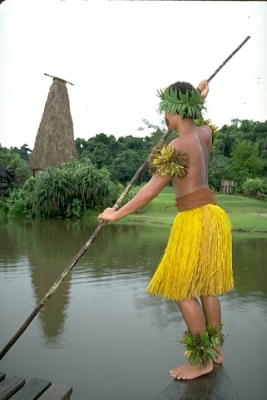
\includegraphics[width=0.25\textwidth]{ch2/0001.jpg}}%
 \hspace{1em}%
  \subcaptionbox{~\inlinecite{Richard2004Statistical}分割结果			   \label{fig:sub:srm}}
      {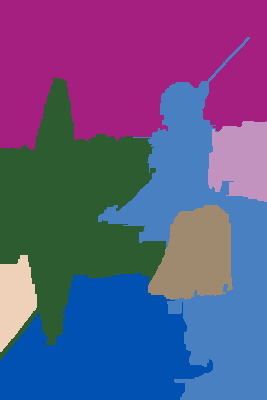
\includegraphics[width=0.25\textwidth]{ch2/srm_7.png}}
 \hspace{1em}
  \subcaptionbox{~\inlinecite{Xiao2015Complexity}分割结果\label{fig:sub:cadm}}
      {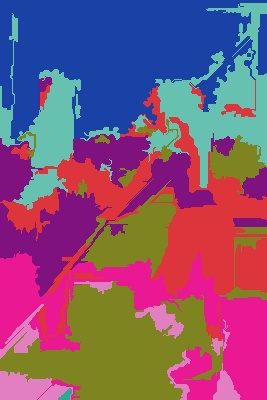
\includegraphics[width=0.25\textwidth]{ch2/cadm.jpg}}
  \caption{基于区域合并的图像分割结果比较}
  \label{fig:rm}
\end{figure}


\section{算法描述}
\label{sec:algorithm}
本章算法主要分为三个阶段,主要流程图如图~\ref{fig:algflow}所示。首先,依据像素的空间相关性和色彩一致性利用文献~\inlinecite{superpixel}的算法对图像进行超像素分割, 将图像分为多个初始区域。 随后,开始第一阶段合并,在此阶段不断将相似的相邻区域进行合并,直到区域数量达到阈值$N$。由于前景的遮挡,可能会使某些背景区域被分割成多个小区域,同时在前一过程中会有一些小区域由于与周围区域差别较大无法参与合并而形成空洞。在第二阶段处理这些遮挡和空洞问题,允许相似但不相邻的区域进行合并,同时将空洞区域与其最相似的邻居区域进行合并。在第三阶段,采用显著性引导的合并策略,分析各区域的显著性,将显著性最差的区域标记为背景区域$R_{B}$,剩下的其它区域一起可以看作是可能的显著性区域。不断以显著性从低到高的顺序依次将所有区域合并到$R_{B}$。最后将在合并过程中可以得到的候选显著性区域(proposals)加权平均得到最终显著性区域结果。\par
\begin{figure}[htb]
  \centering%
      {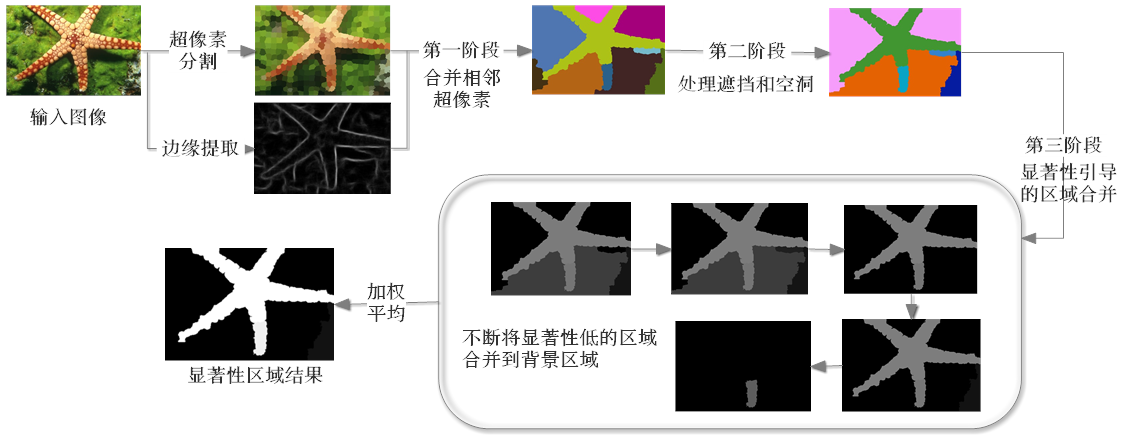
\includegraphics[width=0.9\textwidth]{ch2/SGRMflowChart.png}}

  \caption{算法流程图}
  \label{fig:algflow}
\end{figure}

\par
下面分别详细介绍各阶段的合并规则。

\subsection{第一阶段合并}
\label{subsec:mergeP1}
第一阶段合并只允许相似且相邻的区域进行合并。将区域$i$与区域$j$的合并优先级定义为$PR(i,j)$。计算区域合并的优先级时考虑以下四项因素。
\begin{itemize}
\item 颜色相似性\par
    直观上看,色彩分布一致的区域属于同一对象的概率很大。利用区域颜色直方图的巴氏距离(bhattacharyya distance)来量化区域之间的色彩相似性,越相似的区域合并优先级越高。

    \begin{equation}
    \label{equ:chap2:Pc}
    P_{c}(i,j)=1-HistogramDist(i,j)
    \end{equation}
    其中$HistogramDist$为计算直方图巴氏距离的函数。为了提高效率,利用文献~\inlinecite{ChengPAMI}中提的直方图量化方法对图像色彩空间进行简化处理。在保证覆盖图像中$95\%$以上像素颜色的情况下,去掉图像中出现频次较低的颜色,从而减少直方图的分块(bin)数量以减少计算量。大部分图像在经过处理后的颜色直方图大约包含1000个左右分块。
\item 边缘保持\par
    图像结构化边缘是反映对象边界的重要信息。为了使区域合并过程不破坏对象的边界,在合并优先级中加入边缘保持项,降低区域间的边界包含图像边缘的区域对的优先级。具体其定义为:
    $$P_{e}(i,j)=1-\frac{E(i,j)}{\min(borderLen(i),borderLen(j))}$$
    其中$E(i,j)=\sum_{b\in border(i,j)}Edgeness(b)$,即区域$i$和$j$之间的边界的边缘响应之和, $borderLen(i)$表示区域$i$ 边界的长度(像素数)。本章算法利用文献~\inlinecite{DollarEdge}所提出的算法计算图像的结构化边缘响应,并将其归一化到$[0,1]$之间。
\item 区域空间相关性\par
    区域的空间相关性指区域在空间上的关联性,对于相邻的区域其相关性定义为$$P_{s}(i,j)=borderLen(i,j)/\min⁡(border(i),border(j))$$,其中 $borderLen(i,j)$表示区域$i$和$j$之间边界的长度。区域空间相关性的几何意义为若两区域之间的边界占比越大,说明两区域在空间关系上关联更紧密,因此合并优先级更高。极限情况下,当区域$i$ 完全包含$j$时$P_{s} (i,j)=1$。
\item 区域面积\par
    为了使区域合并在图像全局范围内进行,对面积较小的区域赋予较大优先级。在合并过程中,图像中那些与周围邻域差距较大的区域因为无法进行合并而产生空洞。在合并时考虑区域面积,可以在一定程度上减少空洞的出现。区域面积项的具体定义为:
    $$P_{si}=1-(size(i)+size(j))/TotalSize$$
其中$TotalSize$是图像的总像素数,$size(i),size(j)$表示区域$i,j$的像素数。
\end{itemize}
最终, $PR(i,j)$由上述四项加权平均得到:
\begin{equation}
   \label{equ:chap2:PR}
   PR(i,j)=w_{c}\times P_{c}+w_{e} \times P_{e} + w_{s} \times P_{s} + w_{si} \times P_{si}
\end{equation}
其中加权系数$w_c=0.5, w_e=0.1, w_s=0.2, w_{si}=0.2$为固定值。\par

第一阶段合并过程的具体算法如算法~\ref{alg:algMergeP1}所示。



\renewcommand{\algorithmcfname}{算法}
\begin{algorithm}[htb]
\LinesNumbered
\KwData {初始化区域$Regions$,每次合并的区域比例$k$ ,区域合并目标数$N$ }
\KwResult {合并后的区域$Regions$}
 \While {Size(Regions) > $N$}{
    对每一组相邻区域$i,j$,用公式\ref{equ:chap2:PR}计算合并优先级$PR(i,j)$\;
    根据优先级从大到小对相邻区域对进行排序\;
    选取前面$k\times Size(Regions)$个相邻区域对进行合并\;
    更新区域信息和区域大小\;}
\caption{第一阶段合并算法}
\label{alg:algMergeP1}

\end{algorithm}

\subsection{遮挡和空洞处理}
\label{subsec:mergeP2}

由于前景的遮挡,背景区域通常被分割为多块不相邻的区域,例如图\ref{fig:sub:occ1}中的背景部分,而这些背景部分应该用一个区域表示更合理。另外,在很多情况下背景之间也会出现遮挡情况,例如图\ref{fig:sub:occ2}所示的草地。这两块草地并不相邻,但是从区域合并的角度来说,应该将这两块区域合并到一起。在第一阶段的合并中并不允许不相邻的区域合并,防止在早期将那些属于前景但与局部背景接近的区域合并到背景区域中。在第一阶段合并结束之后处理遮挡则可以有效避免这一错误。本章算法中的遮挡处理的具体算法如算法\ref{alg:algMergeP2}所示。
\begin{figure}[htb]
  \centering%
  \subcaptionbox{背景被前景遮挡\label{fig:sub:occ1}} %标题的长度,超过则会换行,如下一个小图。
    {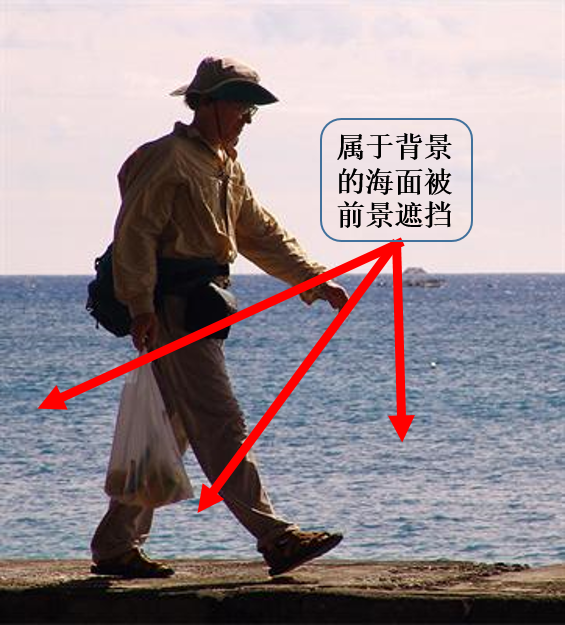
\includegraphics[width=0.4\textwidth]{ch2/occ1.png}}%
 \hspace{1em}%
  \subcaptionbox{其它遮挡情况\label{fig:sub:occ2}}
      {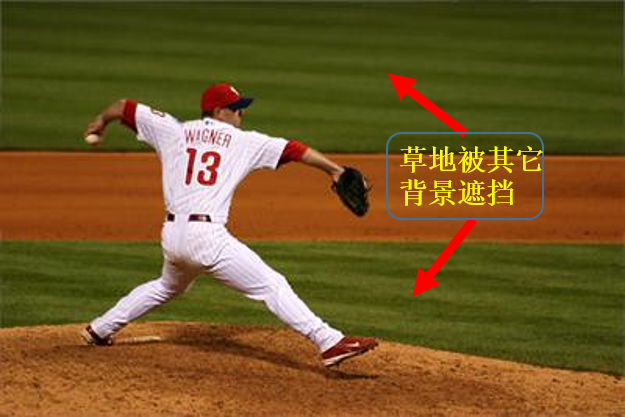
\includegraphics[width=0.4\textwidth]{ch2/occ2.png}}

  \caption{遮挡示例}
  \label{fig:occ}
\end{figure}

\renewcommand{\algorithmcfname}{算法}
\begin{algorithm}[!htbp]
\caption{遮挡处理}
\label{alg:algMergeP2}
%注意label要在caption后面否则引用的时候编号不对
\LinesNumbered
\KwData {图像区域$Regions$, 合并门限$Threshold$ }
\KwResult {合并后的区域$Regions$}
    计算$Regions$中的各区域之间的平均颜色直方图距离$avgDist$\;
    //寻找颜色直方图距离最小的两个区域$minI,minJ$\;
    $minDist = FindMinDist(Regions,minI,minJ)$\;
    $MaxDist = avgDist \times Threshold$\;
    \While{$minDist < MaxDist and Size(Regions)>2$}{
	   合并$minI, minJ$\;
        更新$Regions$\;
        $minDist =FindMinDist(Regions,minI,minJ)$\;}



\end{algorithm}
\par

图像中存在局部小区域,因为与周围邻域色彩分布差别较大,造成优先级低无法参与合并。这些区域将形成空洞,如图~\ref{fig:hole}所示。在图~\ref{fig:sub:hole1}中为输入待处理图像,图像中的显著性前景是小狗,背景部分主要包括草地和小花朵,图~\ref{fig:sub:hole2}中为经过第一阶段合并后得到的区域分割结果,其中用不同颜色标注不同区域。从图~\ref{fig:sub:hole2}中可以看出,因为花朵部分在色彩上与草地区域差距较大,这部分区域没有参与到区域合并中,从而形成了空洞。实际上这些空洞小区域对前景区域和背景区域的合并和分离影响并不大,在处理时将其与其合并优先级最高的邻居区域合并。注意到空洞可能出现在背景以及前景区域,在处理时将其与周围邻域最接近的区域合并可以降低区域复杂度,使得前景区域更容易从背景中分离出来。
\begin{figure}[htb]
  \centering%
  \subcaptionbox{输入图像\label{fig:sub:hole1}} %标题的长度,超过则会换行,如下一个小图。
    {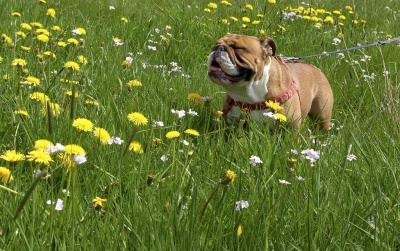
\includegraphics[width=0.4\textwidth]{ch2/hole1.jpg}}%
 \hspace{1em}%
  \subcaptionbox{第一阶段区域合并结果\label{fig:sub:hole2}}
      {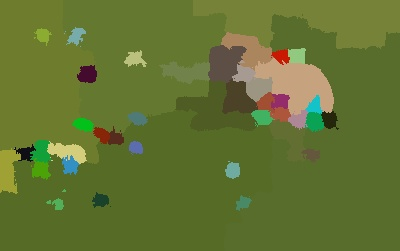
\includegraphics[width=0.4\textwidth]{ch2/hole2.jpg}}

  \caption{空洞示意图}
  \label{fig:hole}
\end{figure}

\subsection{显著性引导的区域合并}
\label{subsec:mergeP3}

在前两个阶段完成后,图像中属于同一对象的像素已经合并到了同一个区域中。第三阶段合并的目标是继续进行区域合并,将图像分为显著性区域和背景区域。与其它大部分基于显著性对象独特性算法不同,本章算法从背景线索入手,不断地将显著性低的区域合并到背景区域。根据观察和实验验证,属于背景的区域主要特点有:
\begin{itemize}
\item (a)连续性强,与周围区域相似度高~\cite{geodesicDistance};
\item (b)靠近图像的边缘~\cite{backgroundPrior};
\item (c)背景区域之间的对比度相对于前景对象较低~\cite{geodesicDistance}。
\end{itemize}

根据(a)和(b),可以推断背景区域易在第一阶段和第二阶段的合并中被合并到包含图像边缘的区域中。因此,选取包含图像边缘像素最多的区域作为背景区域$R_B$。定义区域的显著性值为:
\begin{equation}
   \label{equ:chap2:Saliency}
   Saliency(i)=k_b \times (1-BorderR(i))+ k_a \times (1-AD2C(i)) + k_c \times ContrastB(i)
\end{equation}
其中,$BorderR(i)$表示区域$i$中属于图像边缘的像素占全部图像边缘的比例,$ContrastB(i)=HistogranDist(H(i),H(R_B ))$,即区域$i$与背景区域$R_B$的颜色直方图距离。 $AD2C(i)$为区域$i$中心与图像中心的平均距离,归一化到$[0,1]$范围。在大多数情况下,摄影师在拍摄照片时都会将主体放在靠近中心的位置,因此靠近图像边缘的部分是背景的概率较大。加权系数$k_b,k_a,k_c$为常量,它们的值分别为0.3、0.3、0.4。\par
第三阶段合并的算法如算法~\ref{alg:algMergeP3}所示。
\renewcommand{\algorithmcfname}{算法}
\begin{algorithm}[htb]
\LinesNumbered
\KwData {图像区域$Regions$, 背景区域$R_B$ }
\KwResult {候选显著性区域Proposals}

    \While{$Size(Regions)>2$}{
	   利用公式\ref{equ:chap2:Saliency}计算$Regions$中每个区域$i$的显著性值$S(i)$\;
        寻找显著性值最小的区域$minR$\;
        将$minR$合并到$R_B$\;
        $Proposal = \forall R \in Regions, R \neq  R_B$ \;
        将$Proposal$添加到$Proposals$\;}

\caption{显著性引导的区域合并}
\label{alg:algMergeP3}

\end{algorithm}
\par
在图~\ref{fig:sgrm}中展示了一个显著性引导的区域合并的例子。在图~\ref{fig:sgrm}(a)中是图~\ref{fig:sub:img}经过前两个阶段区域合并后的结果,用不同随机颜色填充不同区域,下同。图~\ref{fig:sgrm}(b)-(h)为显著性引导区域合并的过程。在每次合并时,将当前显著性最弱的区域合并到背景区域,直到只剩2个区域。从图中可以看到,显著性对象直到合并的最后阶段才被合并到背景区域中。虽然合并的最终目标是得到显著性对象和背景两个区域,但是实际上却很难实现。主要原因是在自然图像中,显著性前景自身可能由多个齐次性区域组成,例如图~\ref{fig:sub:img}中的划船人。在实验中,作者发现将显著性对象的各部分合并在一起是十分困难的,主要受到到显著性对象的复杂度和不确定性影响的干扰。因此本章提出以显著性引导的方式,不断将显著性弱的区域合并到背景。合并过程中产生的中间结果以及合并顺序等信息可以用来计算准确的显著性对象区域。

\begin{figure}[htb]
  \centering%
      {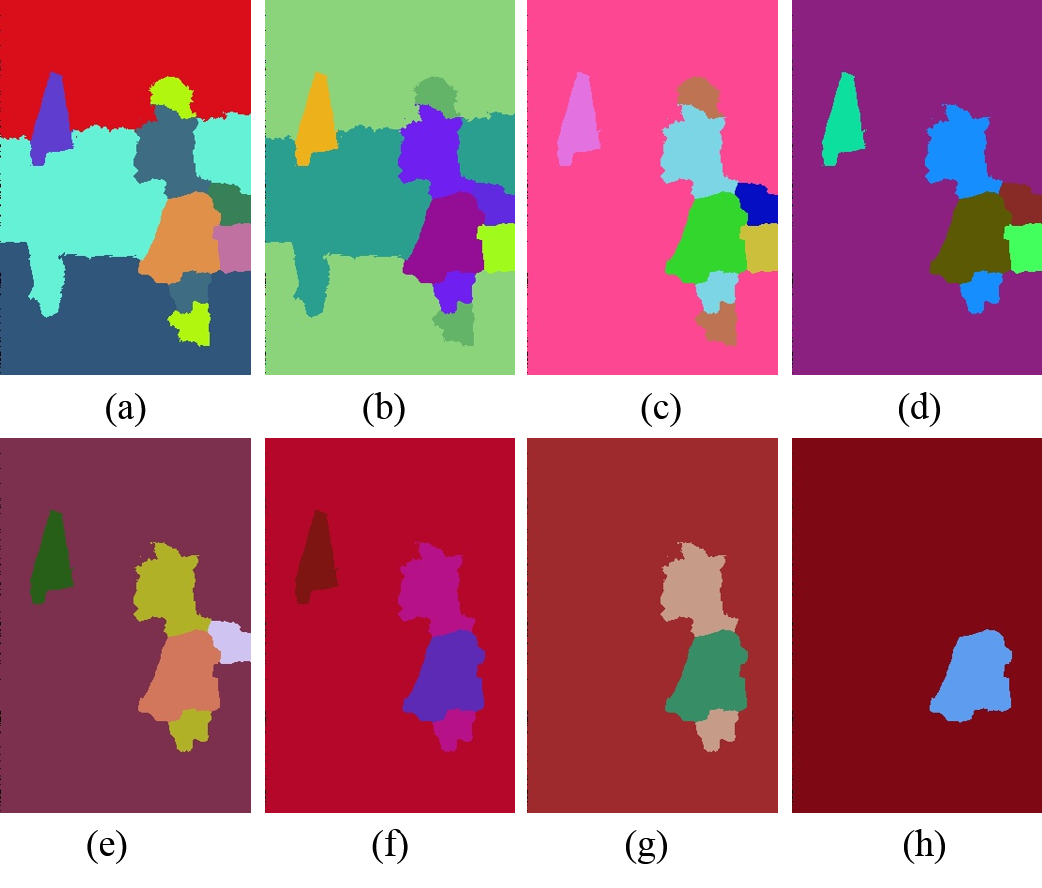
\includegraphics[width=0.9\textwidth]{ch2/sgrm.png}}\\

  \caption{显著性引导的区域合并示意图}
  \label{fig:sgrm}
\end{figure}

\par
\subsection{显著性区域检测}
\label{subsec:saliency}

在自然图像中,前景通常可认为是由多个部分组成,例如人的身体通常可分为皮肤部分、衣服、裤子等。这些部分的颜色和纹理信息等有着较大差别,在合并时很难合并到一起。例如,在图~\ref{fig:sub:fig}中为两幅输入待处理图像,从图像中可以看出上方图像中的显著性对象为红色花朵,下方图像中的显著性对象为两个散步的人。图~\ref{fig:sub:seg}中为经过前两个阶段区域合并后的结果。从图~\ref{fig:sub:fig}中我们看到,经过区域分割之后更容易提取显著性对象。特别是上方图像中的花朵,在区域合并时被分在一个区域,通过比较区域的显著性很容易将其从背景中提取出来。但是,下方图像中的情况更为复杂,从图中易知前景对象是两个穿不同颜色衣裤的人,但是在区域合并时无法将所有属于前景的区域合并在一起。这时,所求显著性对象分布在5个区域之中。

\begin{figure}[htb]
  \centering%
  \subcaptionbox{输入图像\label{fig:sub:fig}} %标题的长度,超过则会换行,如下一个小图。
    {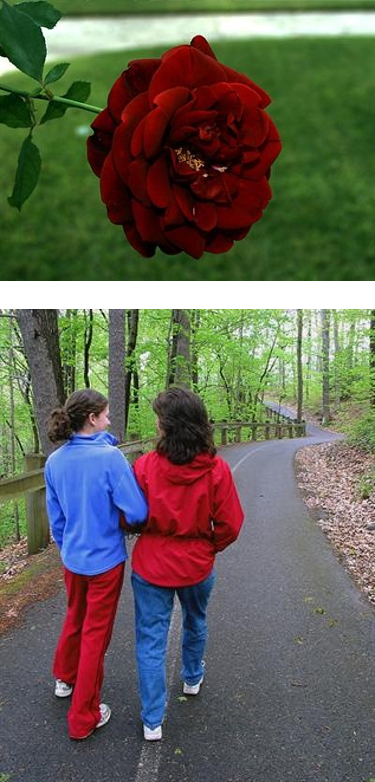
\includegraphics[width=0.25\textwidth]{ch2/fig.png}}%
 \hspace{1em}%
  \subcaptionbox{区域合并结果\label{fig:sub:seg}}
      {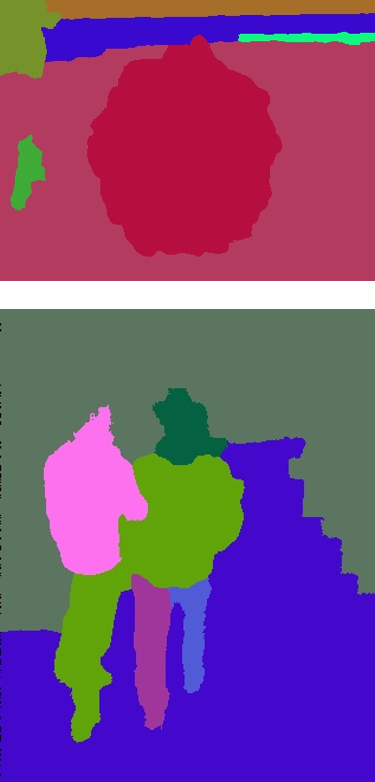
\includegraphics[width=0.25\textwidth]{ch2/seg.png}}

  \caption{齐次的前景区域可以合并到一个区域并易于提取,而非齐次前景对象在区域合并后可能包含多个区域。}
  \label{fig:fgseg}
\end{figure}

\par
为了得到完整的显著性区域,本章算法将第三阶段合并过程中产生的非背景区域作为候选显著性区域(proposals)。假设候选区域$Proposals(i)$包括$k_i$个区域,其中区域$j$的显著性值$PropSal(i,j)$定义为:
$$
   PropSal(i,j)=ContrastB(j) \times \exp{(-\frac{AD2C(j)^2}{\varphi_d^2 })}
$$
其中,$\varphi_d=0.33$为固定值。\par
在合并过程中可以得到多个候选显著性区域,综合考虑候选区域的对比度、形状以及大小等因素对每个候选区域进行可靠性评估,其可靠性值定义为:
\begin{equation}
   \label{equ:chap2:PropSal}
   PropCon(i,j)=w_o \times Obj(i) + w_f \times Fillness(i) + w_{sc} \times Scale(i)
\end{equation}
其中, $Obj(i)$用于评估区域中包含对象的可能性(Objectness)\cite{objectness},具体定义为:
$$Obj(i) = HistogramDist(H(i),H(BoxBorder(i)))$$
设$BB(i)$为包围$Proposals(i)$的最小矩形.上式中$H(BoxBorder(i))=Histogram(p), p \in BB(i)-Proposals(i)$,表示位于$BB(i)$之内区域$Proposals(i)$之外的边界部分像素的直方图。公式\ref{equ:chap2:PropSal}中的$Fillness$定义为:
$$ Fillness(i) = \exp({-(\frac{size(i)}{size(BB(i))}-m_f)^2}/\varphi_f^2)$$ \par

在一般情况下,显著性区域一般形状较为紧凑,假如候选区域中还包括背景区域则会使得$Fillness$值较小。本章中$m_f,\varphi_f$分别为0.56和0.33。 公式\ref{equ:chap2:PropSal}中的最后一项为尺度可靠性,定义为$Scale(i)= \exp(-(size(i)- m_s)^2/\varphi_s^2)$,主要评估显著性区域大小的可靠性,在大多数情况下显著性区域一般只占整个图像的局部,假如候选区域过大则说明其中还包括未合并到背景中的非显著性区域;而如果候选区域过小则说明其可能仅是前景的一部分。本章中$m_s,\varphi_s$分别为0.3和0.5。\par

最后,依据$P$个候选显著性区域及其可靠性指标,以加权平均的方式得到最终显著性结果:
$$ S(I) = \frac{\sum_{i=1}^{P}PropCon(i) \times \sum_{j=1}^{k_i}PropSal(i,j)}{\sum_{i=1}^{P}PropCon(i)}$$

上述过程如图~\ref{fig:weighted}所示,其中将候选显著性区域的可靠性值量化到[0,255]之间,以灰度图格式显示。经过图~\ref{fig:weighted}中左侧的候选显著性区域加权后得到的最终结果如右侧所示。以加权平均的方式计算最终的显著性区域结果可以处理显著性对象分布在多个区域的情况,相比于提取单个显著性区域或者尝试将显著性区域合并到一个区域的方法,该算法的鲁棒性更好。
\begin{figure}[htb]
  \centering%
      {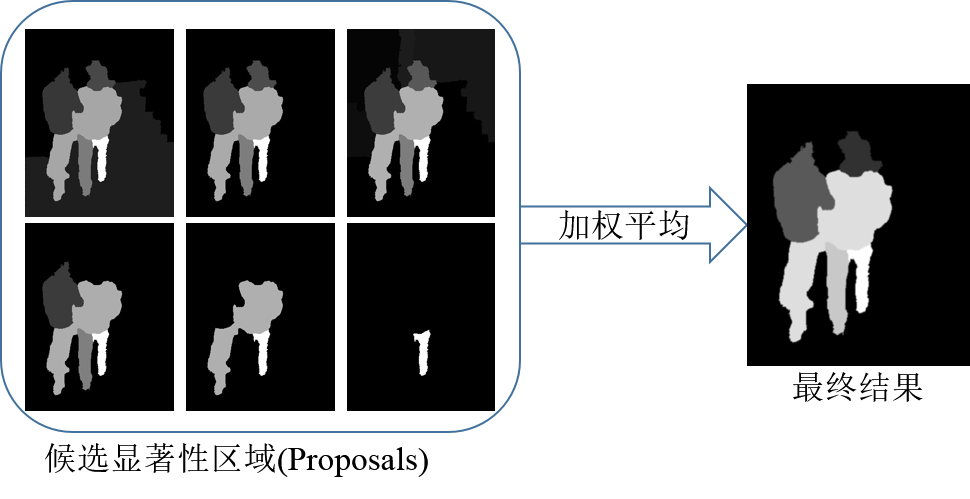
\includegraphics[width=0.9\textwidth]{ch2/weighted.png}}\\

  \caption{显著性引导的区域合并示意图}
  \label{fig:weighted}
\end{figure}

\section{实验结果与分析}
\label{sec:results}


通过C++编程借助OpenCV~\cite{opencv_library}实现了本文算法,在两个公开的测试集ASD~\cite{Achanta08}和ECSSD~\cite{ECSSD}上进行了测试。两个数据集中均包含1000张图像。其中ECSSD数据集中的图像主要是自然场景下拍摄的图像,其背景复杂度相比于ASD数据集中的图像更高,同时也更接近日常实际应用。这两个数据集中均包含人工标注的精确显著性区域。\par
在实验中, 算法~\ref{alg:algMergeP1}中的参数设置为$k=0.2,N=15$,算法~\ref{alg:algMergeP2}中的$threshold=0.8$。公式~\ref{equ:chap2:PropSal}中的系数$w_o,w_f,w_{sc}$分别为0.3、0.05、0.65,在本章所有实验中上述所有参数均使用固定值。

\subsection{显著性检测}
\label{sec:sub:saliencyRst}

为验证本章算法在显著性区域检测中的有效性,将本章所提出的算法 (RM)与AC~\cite{Achanta08}、CHS~\cite{Yan2014Hierarchical}、FT~\cite{saliencyFilter}、GB~\cite{Harel07graph-basedvisual}、GC~\cite{GC},GMR~\cite{GMR},IT~\cite{itti},RC~\cite{ChengPAMI}, SF~\cite{saliencyFilter}、SR~\cite{SR}、DSR~\cite{DSR}、PISA~\cite{PISA}、MC~\cite{MC}等方法进行了比较。其中RC、GMR、CHS、MC算法和本章算法都属于基于区域的方法。部分结果的比较见图~\ref{fig:chap2:comp1}和图~\ref{fig:chap2:comp2},由于早期的AC、IT、SR等算法准确度较低,在图~\ref{fig:chap2:comp1}和图~\ref{fig:chap2:comp2}中只列出了效果更好的6种算法的结果。通过对比可以看到,本章算法可以处理各种复杂背景的自然图像,例如图~\ref{fig:chap2:comp1}中的第三行以及图~\ref{fig:chap2:comp2}中的第二行,对于这些类型的图像RC等算法无法有效工作。而对于背景部分与前景部分在色彩空间分布较为接近的情况,例如图~\ref{fig:chap2:comp1}中的第二行及图~\ref{fig:chap2:comp2}中的第三行,本文算法的处理结果同样优于基于全局对比度的RC等算法。\par
\begin{figure}[h]
  \centering%
      {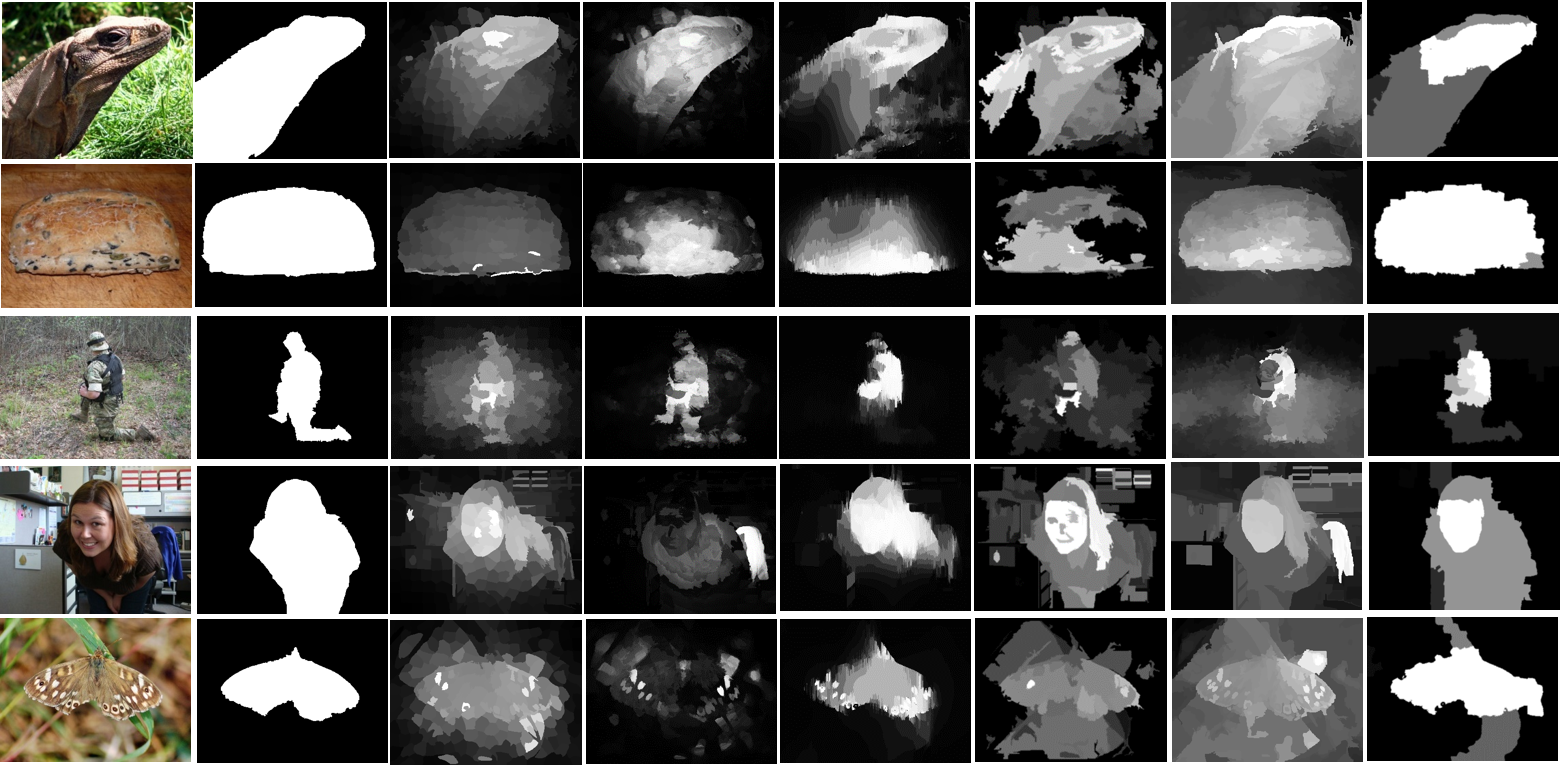
\includegraphics[width=1\textwidth]{ch2/ECSSDRes.png}}\\
(a)输入 (b)正确结果(c)MC \quad (d) DSR \quad (e) PISA \quad (f)RC \quad (g)CHS \quad (h)RM\\
  \caption{ECSSD数据集部分图像显著性检测结果比较}
  \label{fig:chap2:comp1}
\end{figure}
\begin{figure}[h]
  \centering%
      {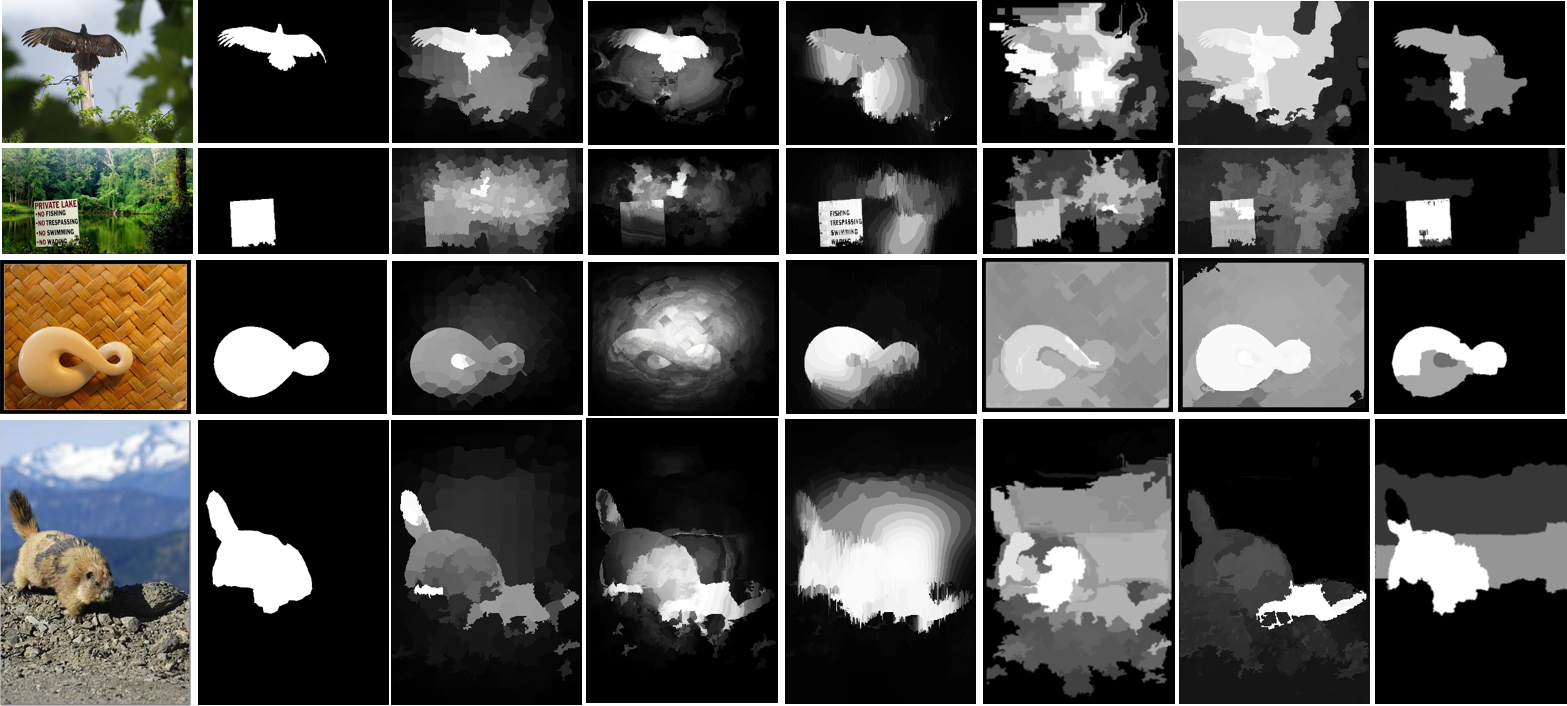
\includegraphics[width=1\textwidth]{ch2/ASDRes.png}}\\
(a)输入 (b)正确结果(c)MC \quad (d) DSR \quad (e) PISA \quad (f)RC \quad (g)CHS \quad (h)RM\\
  \caption{ASD数据集部分图像显著性检测结果比较}
  \label{fig:chap2:comp2}
\end{figure}
为了定量衡量算法的准确性,将显著性检测结果进行二值化后得到的显著性对象与数据集中提供的正确结果进行对比,采用通用的F-Measure值指标来比较算法准确性,其定义为:
$$F_{\beta} = \frac{(1+\beta^2)Precision \times Recall}{\beta^2 \times Precision + Recall}$$
其中$Precision$为精度,$Recall$表示召回率,$\beta^2=0.3$. \par

在实验中,为了消除二值化阈值对结果的影响,将阈值设定为在0到255之间变化,绘制F-Measure随阈值变化的曲线,见图~\ref{fig:sub:ecssdFCurve}和图~\ref{fig:sub:asdFCurve},同时图~\ref{fig:sub:ecssdAvg},~\ref{fig:sub:asdAvg}统计了各方法得到的F-Measure平均值和最大值。通过比较可以看出,本章算法在ECSSD数据集中的F-Measure平均值和最大值略微大于PISA算法,且均优于其他算法, 在ASD数据集中得到的最大F-Measure为0.89, 略低于最高的MC算法(0.91)。 本文算法得到的F-Measure曲线较为扁平, 即F-Measure取值受阈值影响较小, 当阈值门限在128附近时F-Measure可以得到最大值。 比较两个数据集,可以发现ASD数据集中的部分图像背景复杂度较低,因此各算法在ASD数据集上的测试结果均优于ECSSD数据集上的结果。由于本章算法的结果是通过基于超像素的区域合并得到的,显著性值的最小计算单元为超像素,这使得本文算法在ASD数据集中得到的结果的精度要略低于GMR、PISA等算法。 \par
$MAE$是另一个衡量显著性区域检测结果准确性的指标,其定义为:
$$MAE=1/(W\times H) \sum_{x=1}^W\sum_{y=1}^H \| S(x,y)-G(x,y)\|$$ ,其中$W,H$分别为图像的宽和高,$S$为显著性检测结果,$G$为正确值,两者均归一化在[0,1]之间。MAE值越低说明显著性检测误差越小,图~\ref{fig:MAERst}是各算法MAE值在两个数据库中的比较结果。本章算法在ECSSD数据库中的MAE值同样优于其它算法,在ASD数据库中略高于MAE最低的PISA算法。\par
\begin{figure}[h]
  \centering%
  \subcaptionbox{F-Measure曲线\label{fig:sub:ecssdFCurve}} %标题的长度,超过则会换行,如下一个小图。
    {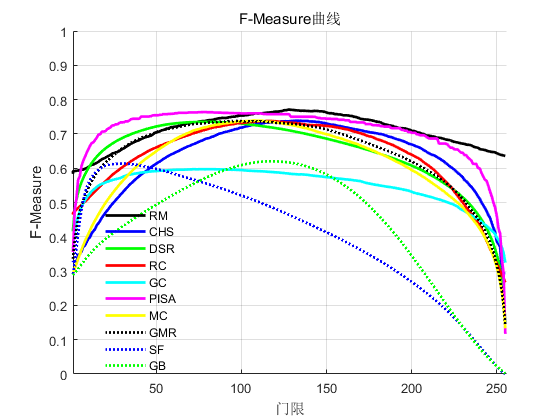
\includegraphics[width=0.45\textwidth]{ch2/FCurve_ECSSD}}%
 %\hspace{1em}%
  \subcaptionbox{平均F-Measure\label{fig:sub:ecssdAvg}}
      {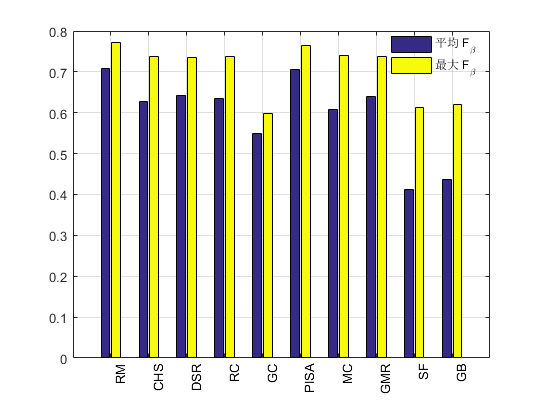
\includegraphics[width=0.45\textwidth]{ch2/FMeasure_ECSSD.png}}
  \caption{ECSSD数据库F-Measure值比较}
  \label{fig:ECSSDRst}
\end{figure}

\begin{figure}[h]
  \centering%
  \subcaptionbox{F-Measure曲线\label{fig:sub:asdFCurve}} %标题的长度,超过则会换行,如下一个小图。
    {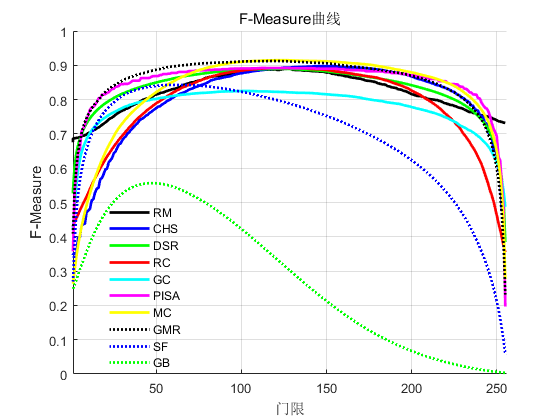
\includegraphics[width=0.45\textwidth]{ch2/FCurve_ASD}}%
 %\hspace{1em}%
  \subcaptionbox{平均F-Measure\label{fig:sub:asdAvg}}
      {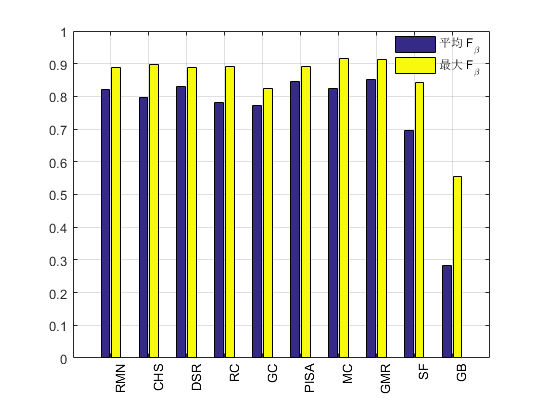
\includegraphics[width=0.45\textwidth]{ch2/FMeasure_ASD.png}}
  \caption{ASD数据库F-Measure值比较}
  \label{fig:ASDRst}
\end{figure}

\begin{figure}[h]
  \centering%
  \subcaptionbox{ECSSD数据集结果\label{fig:sub:ecssdMAE}} %标题的长度,超过则会换行,如下一个小图。
    {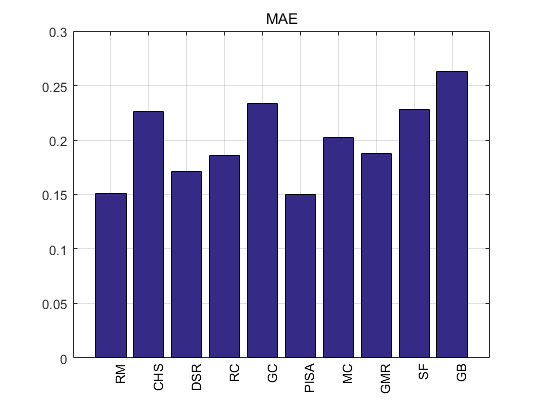
\includegraphics[width=0.45\textwidth]{ch2/ECSSD_MAE.png}}%
 %\hspace{1em}%
  \subcaptionbox{ASD数据集结果\label{fig:sub:asdMAE}}
      {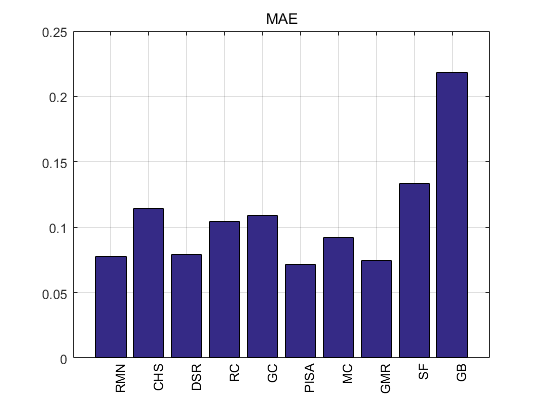
\includegraphics[width=0.45\textwidth]{ch2/ASD_MAE.png}}
  \caption{算法MAE比较}
  \label{fig:MAERst}
\end{figure}

部分算法的速度比较见表~\ref{tab:algTime}.所列数据在配备Intel i7 3.5GHz CPU,16GB RAM的电脑上测得,参与比较的算法均用C++语言实现,其中CHS、RC、PISA和GMR算法均使用作者公开的代码进行测试。ASD数据库和ECSSD数据库中图像大小平均约为$400 \times 300$,表中所列时间为处理每幅图像所用的平均时间。本章算法的速度相比RC和GMR算法稍快,比CHS算法快4倍左右,比与本章算法准确度接近的PISA快7倍左右。\par

\begin{table}[htb]
  \centering

  \caption{算法时间比较}
  \label{tab:algTime}
    \begin{tabularx}{\linewidth}{lXXXXX}
      \toprule[1.5pt]
      {\heiti 算法} & {\heiti RM} & {\heiti CHS} & {\heiti RC} & {\heiti GMR} &{\heiti PISA}\\\midrule[1pt]
      时间(s) & {\bf 0.084} & 0.362 & 0.091 & 0.097&0.583 \\

      \bottomrule[1.5pt]
    \end{tabularx}

\end{table}

\subsection{图像分割结果}
\label{sec:sub:segmentation}

本章所提算法通过区域合并的方式逐渐将图像中相似区域进行合并,在合并过程中可以得到一系列图像分割结果。这些图像分割结果可以为显著性前景检测,对象定位等应用提供重要线索。在本节中,将本章算法与其它图像区域分割算法~\cite{Richard2004Statistical,Xiao2015Complexity,MeanShift}进行比较。在实验中,将图像分割目标设为10。利用各算法进行图像分割时有时不能保证正好得到10个区域,这时选取最接近目标的分割结果作为最终结果。一个好的图像分割算法可以将感兴趣区域其中在一个区域,并且与背景区域分开。如果分割结果所包含的区域过多则包含较多冗余信息,过少则会使得前景区域合并到背景区域中,无法准确提取显著性对象。因此实验中将分割目标设为10左右,基本能同时满足简化图像结构以及保持显著性对象边界的目标。\par
实验中部分比较结果如图~\ref{fig:segCom}所示,其中(a)列图像为输入图像,(b)-(e)列分别为SRM、文献~\inlinecite{Xiao2015Complexity}、Mean Shift~\cite{MeanShift},以及本章算法的分割结果。通过比较可以看出,本章算法的分割结果基本上能够避免将前景对象合并到背景中。而其它图像分割算法均存在将前景对象合并到背景中的情况。主要原因在于这些图像区域分割算法~\cite{Richard2004Statistical,Xiao2015Complexity,MeanShift}在分割时没有考虑到分割过程中不同阶段的特点,始终以同样的策略进行区域合并。另外,在合并过程中没有对遮挡和空洞等情况进行特殊处理。\par
综上所述,本章提出的显著性引导的区域合并算法能够在图像分割过程中较好的保持前景对象的边界,避免其合并到背景区域;同时经过遮挡和空洞处理后,背景区域也可以合并到一起降低了复杂度,有助于显著性前景的提取。
\begin{figure}[htb]
  \centering%
      {\includegraphics[width=0.9\textwidth]{ch2/segcom.png}}\\

  \caption{图像分割效果比较,(a)输入图像,(b)SRM~\cite{Richard2004Statistical},(c)文献~\inlinecite{Xiao2015Complexity},(d)Mean Shift~\cite{MeanShift},(e)本章算法}
  \label{fig:segCom}
\end{figure}


\subsection{算法失败的情况}
\label{subsec:failure}

虽然本章算法可以处理部分复杂背景的情况,但在处理背景连续性较差的图像时效果较差。主要原因是在区域合并的过程中会将前景区域错误的合并到背景中,从而无法提取到正确的前景。例如,在图~\ref{fig:fail}中,(a)和(b)中为输入图像和正确前景,(c)为本章算法第一阶段合并结果,(d)为第二阶段合并结果,(e)为最终提取的显著区域结果。由于这两幅图像中的背景部分十分复杂,并不具备本文假设的连续性。因此在区域合并时误将前景区域合并到了背景中,从而导致算法无法提取正确的显著性前景。
 \begin{figure}[htb]
  \centering%
      {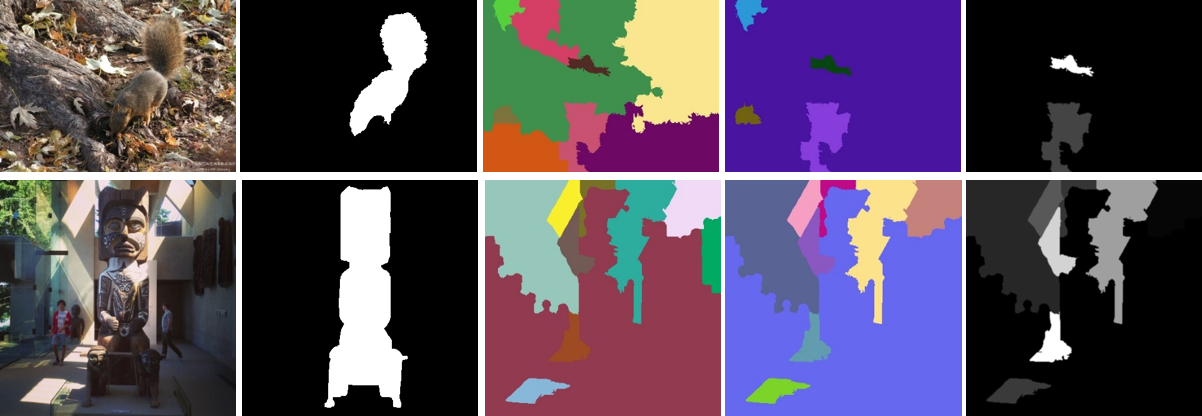
\includegraphics[width=0.9\textwidth]{ch2/fail.png}}\\
(a)输入 \quad\quad \quad(b)正确结果(c)第一阶段合并 (d) 第二阶段合并 (e) 最终结果\\
  \caption{本章算法部分失败例子}
  \label{fig:fail}
\end{figure}


\section{本章小结}
图像显著性区域检测是当前计算机视觉相关领域备受关注的研究热点区域之一。准确提取图像中显著性对象对于图像的识别和理解来说是重要的第一步。虽然人类视觉系统与生俱来就具备这种能力,但是在计算机上实现达到甚至超越人类视觉系统的识别准确度的显著性检测算法却较为困难。虽然近些年提出的一些算法大大提高了图像显著性检测算法的效率和准确度~\cite{ChengPAMI,ufo,Yan2014Hierarchical,geodesicDistance},但是对于一些困难的情况,例如背景复杂度高、前景与背景相近等,目前已有的算法仍无法得到令人满意的结果。\par
本章对图像显著性检测问题进行了研究。借助图像背景线索,以将图像分为显著性对象和背景2个区域为目标,提出了一种基于区域合并的显著性检测算法。由于在区域合并的不同阶段采取了不同的合并策略,本章算法能有效的防止在合并过程中将前景显著性对象错误的合并到背景区域。同时,为了得到准确的显著性对象,本章算法利用背景线索进行区域显著性分析,不断将非显著性区域合并到背景区域。最后,将合并过程中得到的非背景区域作为候选显著性区域,通过加权平均的方式得到最终结果。区别于当前主流算法的主要思路,本章算法采用了基于背景的线索和图像合并的方式提取显著性对象。与前景线索相比,背景线索的通用性更强。图像中的前景对象特征会随着图像内容和应用场景的变化而千变万化,而图像背景部分所具备的连续性强等特点却不会随着图像内容而变化。\par
为了验证本章算法的有效性,在2个公开数据集上测试了本章所提出的算法。实验结果证明了本章所提算法的有效性。在主要是由自然图像构成,难度较大的ECSSD数据集上的实验中,本章算法的准确度和误差指标均优于其他参与比较的算法。本章算法简单直观,且效率高,且易于实现。\par
由于本章所提算法主要基于背景的连续性特点。针对背景连续性不足的图像,目前本章算法无法有效的通过区域合并将背景部分合并在一起,同时可能会将前景错误的合并到背景中。为解决这一问题,在下一步的工作中将考虑引入色彩相似性之外的其它度量方式以及多尺度分析方法来更好的评估图像背景区域之间的相似性。

\chapter{基于样本的快速图像填充}
 \label{cha:Inpainting}
 本章针对图像填充问题进行了研究,提出了一种基于样本的快速图像填充算法。为了使填充后的图像保持图像原有的结构信息,该算法以由粗到精的方式对图像中的缺失部分进行两次填充。在第一次填充时,首先利用离散小波变换(DWT)对输入图像进行预处理。利用DWT的特点,提取低频子带下的低分辨率图像。利用基于样本的填充方法在此低分辨率图像上进行填充。由于低分辨率图像中的高频细节部分已经被去掉,因此第一遍填充的图像的纹理和大部分结构信息都恢复得不错,但是在包含边界的局部区域还存在着一些瑕疵。为了解决这一问题,对原图像进行第二次填充,在这次填充时只处理包含边缘结构信息的部分,使得这部分区域的结构信息能够与图像的其他部分保持连续性。为了提高图像填充的速度,提出了以动态搜索窗口结合分块结构测试的方式来搜索最佳匹配块。实验结果证明,本章所提的算法能够处理各种困难情况,达到了与目前最好的算法相近的效果。但是,本章所提的算法速度明显优于这些算法。
 \section{研究背景}
 \label{background}
 图像填充问题的主要困难在于使得图像中填充后的区域在内容和结构上与周围区域保持连续性以及算法的效率。相比而言,基于样本的算法在处理结构连续性方面更好。基于样本的算法的出发点是图像中缺失部分的像素,可以以分块为单位,利用图像中已知区域中的一个或多个最佳匹配分块来填充。Criminisi等人~\cite{Criminisi04regionfilling}提出了一种基于未知区域边界法线辐射度方向计算填充优先级算法,使得未知区域以一种类似``剥洋葱皮''的顺序进行填充。虽然该算法在一些缺失部分以纹理区域为主的图像中取得了不错的效果,但是对于缺失部分包含明显图像边缘等结构信息的情况却效果不佳。如图~\ref{fig:criminisi}所示,图~\ref{fig:criminisi:1}是待处理图像,其中黑色区域为缺失部分,图~\ref{fig:criminisi:2}为文献~\inlinecite{Criminisi04regionfilling}中算法的处理结果。可以看出,填充后的三角形金字塔尖并没有恢复,填充结果存在明显的不连续情况。Xu等人~\cite{Xu:2010}指出 为了保持结构部分的连续性,应该优先填充那些包含结构信息的分块。对于图~\ref{fig:criminisi:1}中的未知区域,金字塔部分具有明显的边缘结构信息,而天空部分则为平坦的纹理区域。如果在填充时优先填充金字塔部分然后在填充天空部分,则可以避免用包含金字塔部分的分块去填充天空部分。\par
 \begin{figure}[htb]
   \centering%
   \subcaptionbox{输入图像\label{fig:criminisi:1}} %标题的长度,超过则会换行,如下一个小图。
     {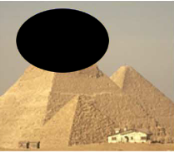
\includegraphics[width=0.3\textwidth]{fillM.png}}%
  \hspace{1em}%
   \subcaptionbox{文献~\inlinecite{Criminisi04regionfilling}算法填充结果\label{fig:criminisi:2}}
       {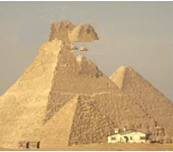
\includegraphics[width=0.3\textwidth]{fillMC.png}}
   \caption{文献~\inlinecite{Criminisi04regionfilling}算法失败例子}
   \label{fig:criminisi}
 \end{figure}
 在基于样本的图像填充算法中,由于像SSD这样的分块相似性度量指标的计算复杂度为$O(N_2)$,且搜索空间为图像全部已知区域,寻找每个缺失部分分块的最佳匹配块是一项非常耗时的工作。对于中等大小的图像,一些算法~\cite{Xu:2010}需要几分钟的时间来处理,这其中大部分时间用于分块的比较和搜索上。在实时或在线图像编辑等实际应用中,用户一般无法忍受超过1分钟的处理时间。\par
 针对以上两方面的问题,本章提出利用基于梯度结构张量(gradient structure tensor,GST)来确定填充顺序,保持填充后图像的结构连续性。为了提高算法速度,提出了一种高效的分块结构测试方法对分块进行结构相似性度量,当分块间的结构信息存在较大差距时可以直接判为不匹配分块,减少冗余的SSD计算。同时,为了减少最佳匹配块的搜索范围,提出了一种动态搜索窗口算法,利用图像的连续性减少搜索范围。在分块匹配时,提出了用加权SSD代替SSD进行,以改进分块间的匹配度。
 \section{相关工作}
 \label{ch3:sec:related}
针对文献~\inlinecite{Criminisi04regionfilling}算法无法处理大面积缺失区域的情况,文献~\cite{Xu:2010}提出 \par
文献\inlinecite{LeMeur_2011}GST \par
文献~\inlinecite{kwokFast}预填充 \par
PatchMatch\cite{Barnes:2009} \par
\inlinecite{LeMeur:2012}算法使用超分辨率算法从填充后低分辨图像中恢复到原图像分辨率
 \section{算法描述}
 \label{ch3:sec:algorithm}
 设输入图像\emph{I} 中包含未知区域 \(\Omega\) 已经已知区域 \(\overline{\Omega}\),本章提出的基于样本的图像填充算法的目标是通过\(\overline{\Omega}\)的信息来计算 \(\Omega\)。和其他经典的基于样本的填充算法那一样,本章所提算法的主要任务是确定填充优先级以及寻找最佳匹配块。
 \subsection{基于GST的填充优先级}
 \label{sec:sub:GST}

 定义未知区域\(\Omega\) 的轮廓为 \(\partial\Omega\), 对于 \(\partial\Omega\)上的每个像素\(p\),将以\(p\)为中心的分块\(\Psi_p\)的填充优先级定义为:
 \begin{equation}
    \label{equ:chap3:order}
    P(p)=C(p)\times D(p)
 \end{equation}

 其中 \(C(p)\) 表示可靠性项\cite{Criminisi04regionfilling},具体定义为: $$C(p)=\frac{\sum_{q\in\Psi_p\bigcap\overline{\Omega}}{C(q)}}{\left\vert{\Psi_p}\right\vert},其中$$\(\left\vert.\right\vert\)  表示计算分块中的像素数. 引入\(C(p)\) 的目的在于让那些包含更多已知像素的区域获得更高的优先级。~\ref{equ:chap3:order}中\(D(p)\) 是数据项,主要评估分块中包含结构信息的情况,增加那些包含较多结构信息分块的填充优先级。Xu等人\cite{Xu:2010}和Lemeur等人\cite{LeMeur_2011}分别提出了不同的\(D(p)\)计算方法。本章中提出了一种基于GST的方法。由于GST可以很好的描述图像的结构信息以及梯度方向,已经被广泛运用于图像处理领域\cite{Kothe03edgeand}。 \par
  对于图像\(I\), 其GST定义为:
  $$T=\left(\begin{array}{cc}T_{11} & T_{12} \\ T_{21} &T_{22}\end{array}\right)=\left(\begin{array}{cc}\overline{I_{\sigma,x}^2} & \overline{I_{\sigma,x}I_{\sigma,y}} \\ \overline{I_{\sigma,x}I_{\sigma,y}} & \overline{I_{\sigma,y}^2}\end{array}\right),$$
  其中 \(I_{\sigma,x}\) and \(I_{\sigma,y}\)  为图像在水平方向和垂直方向上的梯度 ,\(\overline{X}\) 表示高斯核函数\(G_{\hat{\sigma}}\) 与 \(X\)的卷积. \(T\) 的特征值 \(\lambda_1\) 和 \(\lambda_2\) 可以反映图像所包含的结构信息情况。在包含较强边缘信息的区域有 \(\lambda_1>\lambda_2\approx0\) ,而在不含边缘的平坦区域则有\(\lambda_1\approx\lambda_2\approx0\)。 \( \lambda_{1,2} \) 可以通过下式计算: $$\lambda_{1,2}=\frac{1}{2}\left(T_{11}+T_{22}\pm\sqrt{\left(T_{11}-T_{22}\right)^2+4T^2_{12}}\right)$$
  其所包含结构的方向信息可以通过下式计算:
 $$\phi=\frac{1}{2}\arctan{\left(\frac{2T_{12}}{T_{11}-T_{22}}\right)}$$
 为了评估每个分块中是否包含结构信息已经结构的方向信息,LeMeur
 等人\cite{LeMeur_2011}提出计算分块中心点的GST。为了得到区域内更为准确的结构信息,本章算法提出计算分块内所有已知像素的GST,并对结果进行直方图统计。该直方图 \(H\) 以分块内包含的结构方向作为直方图分块依据,统计区域内已知像素的结构能量 \(\lambda_1\)。相比于文献\cite{LeMeur_2011}的方法,本章算法得到的是整个分块的结构信息,比文献\cite{LeMeur_2011}只计算分块中心点的GST的方法更鲁棒。在本章算法中\(H\)的大小(直方图中Bin的数量)为12。定义分块结构能量(patch structure energe, PSE):
 $$P_e\left(p\right)=Max\left(Sum_{b\in{H\left(p\right)}}\left(b\right)\right)$$, 其中\(H\left(p\right)\) 表示结构能量直方图。 对于图像\(I\) , 公式~\ref{equ:chap3:order}中的数据项定义为:
 $$D(p)=(1-\alpha)P_e(p)/max_{q\in{I}}(P_e(q))+\alpha,$$ 其中 \(\alpha\) 是一个线性变换因子,使得\(D(p)\in{[\alpha,1]}\)。加入\(\alpha\) 的目的是使得数据项的值接近于可靠性项值。在本章算法中,按照参考文献\cite{Xu:2010}中的建议将\(\alpha\)设为固定值0.2。
 \subsection{加权SSD}
 \label{sec:sub:WSSD}
 为了寻找样本分块\(\Psi_p\)的最佳匹配块,Criminisi等人\cite{Criminisi04regionfilling}借助于两个分块间已知像素的SSD类评估分块间的相似性。待填充分块\(\Psi_p\)的最佳匹配块定义为
 \begin{equation}
 \label{equ:cha03:bestmatch}
 \Psi_{\hat{q}}=arg\;min_{\Psi_q\in\Phi}d(K(\Psi_p),K(\Psi_q))
 \end{equation}
 其中,\(d(.,.)\) 表示计算两个分块之间的 SSD , \(K\)表示提取分块内的已知像素的操作 , \(\Phi\)表示搜索范围。实际上,仅仅依靠分块已知区域的SSD是无法保证找到的最佳匹配快都是最合适用于填充的分块。例如,如图~\ref{cha03:fig:1} 所示,蓝色的分块为待填充分块,绿色分块为用公式~\ref{equ:cha03:bestmatch}计算得到的最佳匹配块。在图~\ref{cha03:fig:1}左边部分图像中绿色的分块中包含了栏杆,而待填充分块主要是草地;右边部分图像中绿色分块中包含了部分树枝区域,而蓝色的待填充区域主要是天空背景。假如利用绿色分块的对应像素对蓝色分块进行填充会导致将错误的结构信息填充到未知区域,造成最终的填充结果出现明显的不连续现象。在一些情况下仅靠分块已知区域的SSD 不能找到合适的最佳匹配块对缺失部分进行填充。
 \begin{figure}[!htbp]
 	\begin{center}
 			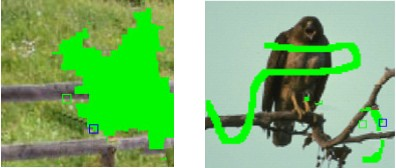
\includegraphics[width=0.8\columnwidth]{ch3/fig1.jpg}
 	\end{center}
     \caption{使用已知分块内SSD搜索造成错误匹配情况}
 	\label{cha03:fig:1}
 \end{figure}
 在文献 \inlinecite{kwokFast}中,提出了一种基于梯度的预填充方法,对待填充分块内的未知像素进行估计。基于同样的预处理方法,文献\inlinecite{jemi:2011}提出使用已知和未知区域的加权SSD (Weighted SSD,WSSD)来寻找最佳匹配块。该算法的预填充算法假设未知区域内的像素梯度值为零。基于这一假设,未知区域的像素颜色值可以通过梯度方程的最小二乘法来求解。然而,实际应用中图像较难满足梯度值为零这一假设。这这种预处理方法只考虑了分块内的局部梯度信息,最终的预处理结果并不明显。 Xu等人\cite{Xu:2010}指出,待填充分块内新填充的像素应该与周围分块保持颜色一致性和连续性。基于这一思路,本章提出了一种新的预处理方法。
 为了方便比较,本章中使用与文献\inlinecite{Xu:2010}一致的符号标识。假设 \(N(p)\) 为中心点在\(p\)的邻域窗口,集合\(N_s(p)\)定义为:
 $$N_s(p)= \left\{ p_j:p_j \in N(p)\;and\;\Psi_{p_j} \subset \overline{\Omega} \right\}.$$
 分块 \(\Psi_p\) 和\(\Psi_{p_j}\)  之间的相似性定义为:
 $$\omega_{p,p_{j}}=\frac{1}{Z(p)}exp\left(-\frac{d(K\Psi_p,K\Psi_{p_j})}{\sigma^2\left|K\Psi_p\right|}\right)$$
 其中 \(Z(p)\) 为归一化因子使得 $$\sum_{p_j\in N_s(p)}\omega_{p,p_j} = 1$$ , \(\sigma\) 为固定值5.0 \cite{Xu:2010}.\par
 令运算符\(U\) 表示从分块中提取未知像素,分块 \(\Psi_p\) 中的未知像素的预填充为
 $$U(p)=U\left(\sum_{p_j \in N_s(p)}{\omega_{p,p_j}\Psi_{p_j}}\right)$$\par
 为了寻找待填充分块的最佳匹配块, 本章提出以WSSD的方式来评估分块之间的相似性:
 \begin{equation}
 W(\Psi_p,\Psi_{p_j})=\beta\times d(K(\Psi_p),K(\Psi_{p_j}))+(1-\beta)\times d(U(\Psi_p),U(\Psi_{p_j}))
 \label{chap03:equ:wssd}
 \end{equation}
 其中加权系数 \(\beta\) 为已知区域的权值,从公式~\ref{chap03:equ:wssd}中可看出WSSD综合考虑了分块未知区域和已知区域的信息。由于未知区域是通过预填充算法估算的,因此加权系数\(\beta\)的值应该大于0.5,以使得已知部分的权值更大。在本章算法中 \(\beta\)的值建议范围为$[0.8, 0.9]$。综上所述,分块\(\Psi_p\) 的最佳匹配块定义为:


 $$\Psi_{\hat{p}}=arg\;min_{\Psi_q \in \Phi}{W(\Psi_p,\Psi_q)}.$$


 \subsection{最佳匹配块搜索策略}
 在基于样本的图像填充算法中,主要的计算量集中在最佳匹配块的搜索中。为了提高搜索速度,文献\cite{kwokFast}提出了一种基于$K$D-tree的近似最相近邻域搜索算法,该方法主要利用高效的$K$D-tree数据结构对搜索进行加速。本章算法中,以让搜索更智能和更快为目标,提出一种智能搜索策略。由于SSD计算需要对分块每个像素进行比较,效率很低。实际上,我们人眼在搜索匹配块时并不会这样逐个像素去比较。只有当两个分块在外观上十分接近时,才可能进行这样逐个像素的比较。假如要人工完成最佳匹配块的搜索工作,人们会首先将那些明显不一致的分块放到一边不予考虑。这个预先判断和筛选的过程非常重要,本章提出利用分块结构测试的方式对分块进行测试,判断分块间结构信息是否一致。对于那些在结构上明显不一致的分块,可以直接将其排除在外,减少冗余的计算,从而加快搜索的速度。
 \subsubsection{分块结构距离测试}
 \label{sec:subsub:PST}
 在~\ref{sec:sub:GST}中,分块GST直方图被用于描述分块的结构信息。对于相似的分块,他们之间的SSD会相对较小,因此他们一定包含相似的结构信息。例如,同为不包含结构信息的两块纹理信息为主的分块,或者同为包含垂直方向边缘结构信息的分块等。对于这些相似的分块,他们的分块直方图分布也会比较相似。假如两个分块\(\Psi_p\) 、\(\Psi_q\)的GST直方图分别为 \(H(p)\) 和 \(H(q)\),本章算法将他们之间的分块结构距离(patch structure distance, PSD)定义为\(H(p)\) 和\(H(q)\)之间的相关系数,即:

 $$PSD(p,q)=\frac{\acute{\sigma}_{pq}+c}{\acute{\sigma_p}\acute{\sigma_q}+c},$$
其中\(\acute{\sigma}_{pq}\) 为 \(H(p)\)与 \(H(q)\)之间的协方差, \(\acute{\sigma_p}\) 及 \(\acute{\sigma_q}\) 分别为 \(H(p)\) 与\(H(q)\)的标准差, \(c\) 是一个很小的常数避免出现零除以零的情况。\par
 对于待填充分块 \(p\)以及搜索窗口内的分块\(q\),当\(PSD(p,q)\)大于某门限,本章算法中门限值设置为(0.5\(\sim\)0.6), 那么认为\(p\) 和 \(q\)在结构上存在较大差异,这也就意味着\(q\) 不可能是要寻找的最佳匹配块。这时也就没有必要再去计算他们之间的SSD。 基于此,对于候选分块\(c\),在计算 \(p\) 与 \(c\)之间的SSD时,首先测试这两者之间的PSD值是否在可接受的范围之内。对于通过PSD测试的分块,再通过SSD进一步评估分块之间的相似性,而PSD测试没有通过的分块可以直接忽略。由于\(\overline{\Omega}\)范围内所有分块的分块GST直方图可以预先计算,且PSD的计算复杂度远低于SSD, 引入PSD测试可以节省很多SSD的冗余计算。\par
例如,在图~\ref{chap03:fig:PSD}中, 蓝色的分块为待填充分块,绿色矩形之内为最佳匹配块搜索范围, 红色分块为通过PSD测试的候选分块,黑色分块为本章算法搜索到的最佳匹配。从图~\ref{chap03:fig:PSD}中可以看到,由于蓝色的待填充分块包含垂直方向的边缘,所有包含水平方向边缘的分块均没有通过PSD测试。因此这些分块不可能是最佳匹配分块目标,可以直接忽略。
 \begin{figure}[!htbp]
 	\begin{center}
 			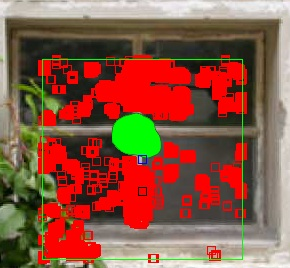
\includegraphics[width=0.6\columnwidth]{ch3/fig2.jpg}
 	\end{center}
     \caption{PSD测试示意图}
 	\label{chap03:fig:PSD}
 \end{figure}


 \subsubsection{动态搜索窗口}
 \label{sec:subsub:dynamicSearch}
 在传统的基于样本的图像填充算法中,公式~\ref{equ:cha03:bestmatch}中的 \(\Phi\)为以每个待填充区域为中心的固定窗口\cite{LeMeur_2011},或者是全部未知区域\inlinecite{Criminisi04regionfilling}。 设 \(\Psi_p\) 为中心在\(p\)处的待填充分块,考虑到图像局部范围的连续性,在\(p\)附近找到\(p\)的最佳匹配块的概率应该较大。因此定义局部窗口
 $$Win_l(p)=Win(p,sizeL)\cap \Omega,$$
 其中 \(Win(p,sizeL)\) 是大小为 \(sizeL\times sizeL\)中心点在 \( p\)的矩形窗口. \par
受到快速近似最相似邻域搜索算法PatchMatch \cite{Barnes:2009}的启发,利用图像的连续性特点,本章提出了利用邻域窗来提高搜索效率。假设 \(\Psi_q\)为 \(\Psi_p\)的相邻分块 ,即\(p\) 与\(q\)之间的距离与分块大小相等。如果 \(\Psi_q\) 已经完成了填充 ,且其最佳匹配快为 \(\hat{q}\)。那么根据图像的连续性特点,  相邻分块\(\Psi_p\)的最佳匹配块与 \(\hat{q}\)相邻的概率也会较大。 因此,定义邻域搜索窗口如下:
 $$Win_n(p)=Win(\hat{q},sizeN)\cap\Omega.$$
 当\(p\)的相邻分块中还没有一个完成填充时,\( Win_n(p)=\emptyset  \)。结合局部窗口全部搜索区域定义为:
 $$\Phi=Win_n(p)\cup Win_l(p).$$
 在图\ref{ch3:fig:3}中展示了搜索范围的一个例子。图\ref{ch3:fig:3}中,蓝色的分块为待填充分块,邻域搜索窗口和局部搜索窗口分别用红色和绿色标识,搜索到的最佳匹配块用黑色标识 。通过这种搜索方式,在图像填充过程中每个分块的最佳匹配块可以在更小的动态范围内被搜索到。因为邻域窗口的引入,局部窗口的大小可以设置得更小。在本章算法中,局部窗口和邻域窗口分别被设置为8\(\sim\)10 以及5\(\sim\)7 倍的分块大小。对于那些邻域窗口为零的分块,可以增大其局部搜索窗口的大小。\par
 \begin{figure}[!htbp]
 	\begin{center}
 			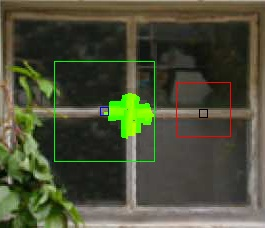
\includegraphics[width=0.6\columnwidth]{ch3/fig3.jpg}
 	\end{center}
     \caption{局部搜索窗口与邻域搜索窗口}
 	\label{ch3:fig:3}
 \end{figure}
 综上所述,本章提出的改进的基于样本的图像填充算法见算法\ref{ch3:alg:inpainting}。
 \renewcommand{\algorithmcfname}{算法}
\begin{algorithm}[!htbp]
\LinesNumbered
\KwData { 图像 \(I\),其中未知区域 \(\Omega \) ,已知区域 \(\overline{\Omega}\),  \(\Omega \) 的轮廓为 \(\partial \Omega\)}
\KwResult {填充后的图像}

   \ForEach {分块 $\Psi_q \in \overline{\Omega}$ }{
   计算分块能量直方图\(H(q)\)\;}

   \ForEach { \(\partial \Omega\)上的像素 \(p\) }{
   	 计算以$p$为中心的分块\(\Psi_p\)\ 的结构能量直方图以及PSE\;
   	 计算\(\Psi_p\) 的填充优先级 $Pri[\Psi_p]$\;}
   \While{\( \Omega \neq null\) }{
	$\Psi = \arg max_{p \in \partial \Omega}Pri[p]$\;
    按照 \ref{sec:sub:dynamicSearch} 中的方法计算搜索窗口\(\Phi\) \;
    \ForEach {$\Psi_q$ in \(\Phi\)}{
    $d = PSD( \Psi_q,\Psi)$\;
     	\If{d < threshold}
     		{利用公式\ref{chap03:equ:wssd}计算$wd[\Psi_q]=WSSD(\Psi_q,\Psi)$\;}
     	
     	 \Else
     	 	{ $wd[\Psi_q]=MAX$\;}
     $\Psi_m = \arg min_{p \in \phi }wd[p]$ \;
     利用 \(\Psi_m\)的对应像素填充 \(\Psi\) 中的缺失部分\;
     更新\(\partial \Omega\)\;
     \ForEach{\(\partial \Omega\) 上新增像素\(n\) }
     {
     计算 \(\Psi_n\)的填充优先级$Pri[\Psi_n]$\;
     }
   }
   }
\label{ch3:alg:inpainting}
\caption{基于样本的图像填充}
\end{algorithm}

\subsection{两阶段由粗到精图像填充}
\label{sec:2.2}
对于图像填充算法来说,主要的困难在于保持输入图像中连续的结构和纹理信息以及尽可能减少图像填充过程的运算量。为了加快算法的速度,首先对输入图像进行预处理,降低其分辨率。 对输入图像进行DWT,选取低频子带图像作为输入图像的低分辨率版本。由于DWT的低频部分可以保留图像中的结构信息,因此在此低分辨率版本图像上进行填充可以保持原图中的结构信息。并且,由于低分辨率图像大小是原图像的四分之一, 使得填充速度是原图像的四倍。\par
在文献\inlinecite{LeMeur:2012}中,提出了一种与本章算法类似的两阶段填充算法,不同之处是文献\inlinecite{LeMeur:2012}算法使用超分辨率算法从填充后低分辨图像中恢复到原图像分辨率。虽然低分辨率下填充算法可以更快,但是由于随后的超分辨率算法耗时远大于填充算法,造成整个算法并没有加快速度 。与文献\inlinecite{LeMeur:2012}不同,本章算法中输入图像可以与低分辨率图像同时填充。例如,在图~\ref{ch3:fig:4}中,左边的图像\(C\)为输入图像的低分辨率版本,右边图像为相应的输入图像\(O\); 假如图像\(C\)中的分块 \(\Psi_c\) 位于 \((x,y)\), 其最佳匹配块\(\Psi_{\hat{c}}\) 的位置位于 \((i, j)\),那么图像 \(O\)中位于 \((2x, 2y)\)处的对应分块\(\Psi_o\) 可以通过 位于\((2i, 2j)\)处的相应最佳匹配块\(\Psi_{\hat{o}}\) 来进行填充。\par
\begin{figure}[!htbp]
	\begin{center}
			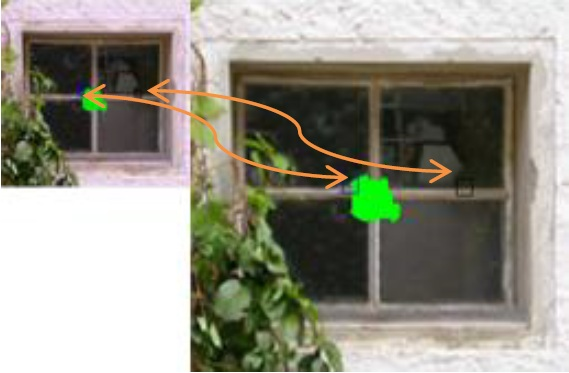
\includegraphics[width=0.6\textwidth]{ch3/fig4.jpg}
	\end{center}
    \caption{基于低分辨率版本的同步填充}
	\label{ch3:fig:4}
\end{figure}

本章提出的两阶段图像填充算法如图~\ref{ch3:fig:5}所示。在第一次填充时,低分辨率版本图像和原输入图像根据低分辨率图像填充过程进行同步填充,只取原分辨率图像的填充结果进行下一步填充。如图~\ref{ch3:fig:5}中间部分所示,第一次填充后的结果在大部分区域可以保持纹理和结构信息的连续性,但是在一些包含边缘信息的部分(见红色方框内右上角显示的放大版本)还存在一些不连续的情况。为了处理这一问题,本章算法在这些区域再进行第二阶段填充。利用PSE可以对这些包含边缘信息且存在结构不连续的区域进行定位。需要进行第二次填充的区域定义为: $$\forall p \in \Omega, P_e(p)>E_{Thres}$$。在本章算法中 \(E_{Thres}\) 设置为\(0.015 \times Max_{q\in{I}}{(P_e(p)})\)。在图~\ref{ch3:fig:5}的中间部分,可以看到需要进行第二次填充的区域小于原始区域,并且只覆盖了包含瑕疵的那部分范围。在第一次填充中,未知区域的像素已经通过预填充进行了估算,在第二次填充时则可以直接利用第一次填充的结果作为预填充结果,因此可以节省一次预填充过程。

% For one-column wide figures use
\begin{figure}[!htbp]
\begin{center}
% Use the relevant command to insert your figure file.
% For example, with the graphicx package use
  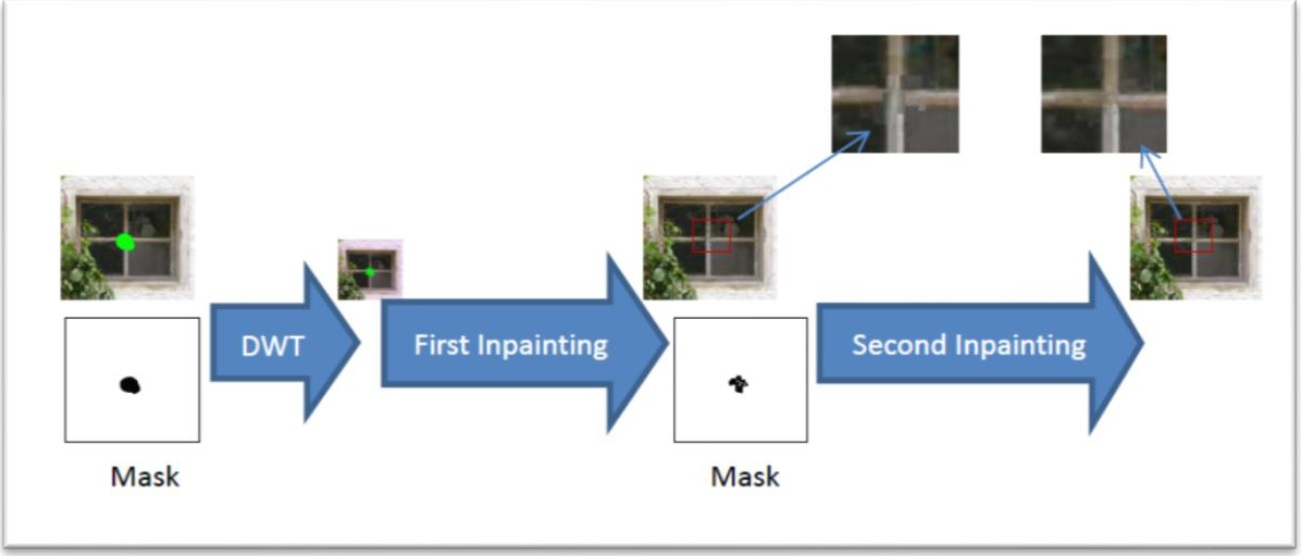
\includegraphics[width=1.0\textwidth]{ch3/fig5.jpg}
% figure caption is below the figure
\end{center}
\caption{两阶段填充示意图}
\label{ch3:fig:5}       % Give a unique label
\end{figure}

 \section{实验结果与分析}
 \label{cha3:results}
为了验证本章所提算法的有效性,在大量自然图像上进行了实验。部分结果以及和现有其他算法\cite{Criminisi04regionfilling,Xu:2010}的比较如图~\ref{ch3:fig:6}所示。在实验中,第一遍填充时分块的大小设置为\(7\times7\) ,第二次填充时设置为 \(9\times9\)。和文献~\inlinecite{Xu:2010}中一样,本章所提算法中\(N_s(p)\)值设置为51。本章算法通过 C++语言实现,所有实验结果通过一台配备  Intel 2.67 GHz CPU ,512MB内存的PC上得到。\par


在图~\ref{ch3:fig:6}中,可以看到本文算法得到的填充结果可以有效的利用连续性强的结构和纹理信息对未知区域进行填充。与文献~\inlinecite{Criminisi04regionfilling}中算法相比,本文算法填充的图像效果更好,与文献~\inlinecite{Xu:2010}填充效果基本接近。\par
算法的时间比较如表~\ref{ch3:tab:timing}所示,其中所列的图像与图~\ref{ch3:fig:6}一一对应。由于计算复杂度更低,本章所提出的两阶段填充算法比文献 \inlinecite{Criminisi04regionfilling,Xu:2010}的算法更快。这主要归功于本章算法基于多分辨率的两步填充、动态搜索窗口以及PSD测试方法。
\begin{table}[htb]
\begin{center}
% table caption is above the table
\caption{算法时间比较}
\label{ch3:tab:timing}       % Give a unique label
% For LaTeX tables use
\begin{tabular}{lllll} \hline
\multicolumn{1}{c}{\multirow {2}{*}{图像}}&\multicolumn{1}{c}{\multirow {2}{*}{未知区域像素数}}& \multicolumn{3}{c}{时间(单位:秒)}\\
\cline{3-5}
\multicolumn{1}{c}{}&\multicolumn{1}{c}{}& \multicolumn{1}{c}{~\inlinecite{Criminisi04regionfilling}} &~\inlinecite{Xu:2010}&本章算法\\
\hline
\multicolumn{1}{c}{Pyramid} & \multicolumn{1}{c}{19636} & \multicolumn{1}{c}{83} &\multicolumn{1}{c}{143}& \multicolumn{1}{c}{9}\\				
\multicolumn{1}{c}{Plane} & \multicolumn{1}{c}{17914} & \multicolumn{1}{c}{82} &\multicolumn{1}{c}{130}& \multicolumn{1}{c}{10}\\				
\multicolumn{1}{c}{Riding} & \multicolumn{1}{c}{23161} & \multicolumn{1}{c}{121} &\multicolumn{1}{c}{165}& \multicolumn{1}{c}{25}\\
\multicolumn{1}{c}{Eagle} & \multicolumn{1}{c}{14837} & \multicolumn{1}{c}{84} &\multicolumn{1}{c}{108}& \multicolumn{1}{c}{17}\\
\multicolumn{1}{c}{Beach} & \multicolumn{1}{c}{6281} & \multicolumn{1}{c}{17} &\multicolumn{1}{c}{45}& \multicolumn{1}{c}{4}\\
\hline
\end{tabular}
\end{center}
\end{table}


\begin{figure}[htbp]
\begin{center}
% Use the relevant command to insert your figure file.
% For example, with the graphicx package use
  \includegraphics[width=1.0\textwidth]{ch3/fig6f.jpg}\\
  (a) 待填充图像 (b) 文献\inlinecite{Criminisi04regionfilling}算法结果  (c) 文献\inlinecite{Xu:2010}算法结果  (d) 本章算法结果
% figure caption is below the figure
\end{center}
\caption{与文献\inlinecite{Criminisi04regionfilling} 和 ~\inlinecite{Xu:2010}算法比较结果}
\label{ch3:fig:6}       % Give a unique label
\end{figure}




为了进一步验证算法的有效性,本章所提算法对文献\inlinecite{LeMeur_2011,kwokFast,LeMeur:2012}中的一些困难的例子进行了实验和对比,结果分别如图~\ref{ch3:fig:7},~\ref{ch3:fig:8},~\ref{ch3:fig:9}所示。从这些图中可以看到,由于采用了基于GST的填充优先级策略,本章算法填充后的图像可以保持原图像中那些明显的边缘部分的连续性,特别是在图中红色矩形框所标注区域。从图 ~\ref{ch3:fig:8}及图\ref{ch3:fig:9}中可以看到,本章所提算法对于那些主要由纹理构成的图像时会产生重复的纹理模式。主要原因是最佳匹配块搜寻过程中使用了基于邻域的搜索窗口。\par
\begin{figure}[!htbp]
\begin{center}
% Use the relevant command to insert your figure file.
% For example, with the graphicx package use
  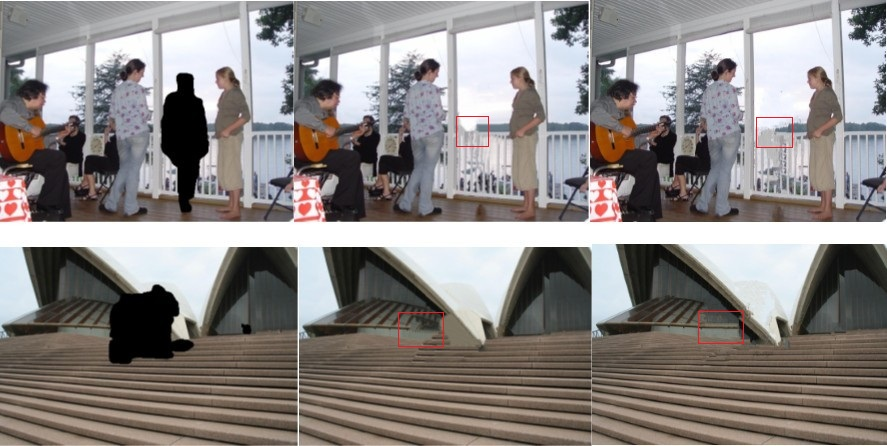
\includegraphics[width=0.8\textwidth]{ch3/fig7.jpg}\\
  (a) 待填充图像 (b) 文献\inlinecite{LeMeur_2011}算法结果    (c) 本章算法结果
% figure caption is below the figure
\end{center}
\caption{与文献~\inlinecite{LeMeur_2011}算法比较结果}
\label{ch3:fig:7}       % Give a unique label
\end{figure}
\begin{figure}[!htbp]
\begin{center}
% Use the relevant command to insert your figure file.
% For example, with the graphicx package use
  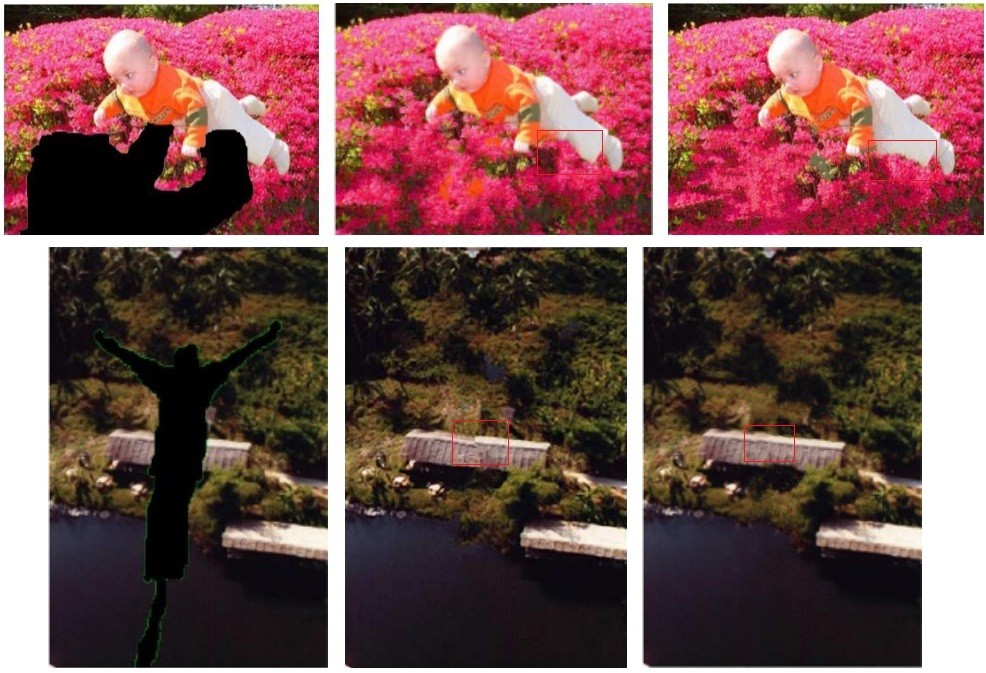
\includegraphics[width=0.8\textwidth]{ch3/fig8.jpg}
  \\
  (a) 待填充图像 (b) 文献\inlinecite{kwokFast}算法结果    (c) 本章算法结果
% figure caption is below the figure
\end{center}
\caption{与文献~\inlinecite{kwokFast}算法比较结果}
\label{ch3:fig:8}       % Give a unique label
\end{figure}

\begin{figure}[!htbp]
\begin{center}
% Use the relevant command to insert your figure file.
% For example, with the graphicx package use
  \includegraphics[width=0.8\textwidth]{ch3/fig9.jpg}
  \\
  (a) 待填充图像 (b) 文献\inlinecite{LeMeur:2012}算法结果    (c) 本章算法结果
% figure caption is below the figure
\end{center}
\caption{与文献~\inlinecite{LeMeur:2012}算法比较结果}
\label{ch3:fig:9}       % Give a unique label
\end{figure}

PatchMatch算法~\cite{Barnes:2009}已经被用于著名图像处理软件 Adobe Photoshop中的``内容感知的区域填充''功能当中。PatchMatch算法可以实现人机交互的快速填充,当待填充部分区域较小且图像中没有明显的结构信息时该算法的填充效果较好。但是,当图像中缺失部分面积过大,或图像中包含明显结构时,PatchMatch算法并不能得到满意的效果。将本章算法和PatchMatch算法针对这些困难情况进行了测试和对比,部分结果如图~\ref{ch3:fig:10} 所示,其中中间一列为PatchMatch算法填充结果,最后一列为本章算法填充结果。图~\ref{ch3:fig:10} 中的红色矩形框中显示,PatchMatch算法填充结果无法保存图像在结构上的连续性,例如在第一行和第二行图像中的栏杆部位、第三行图像中的树枝处。本章算法在这些区域的填充效果较好,可以保持栏杆等结构区域的连续性。
\begin{figure}[!htbp]
\begin{center}
% Use the relevant command to insert your figure file.
% For example, with the graphicx package use
  \includegraphics[width=0.8\textwidth]{ch3/VsAdobe.png}
% figure caption is below the figure
 \\
  (a) 待填充图像 (b) PatchMatch 算法\cite{Barnes:2009}结果    (c) 本章算法结果
\end{center}
\caption{与PatchMatch~\cite{Barnes:2009}算法比较结果}
\label{ch3:fig:10}       % Give a unique label
\end{figure}\par

 \section{本章小结}
 \label{cha3:conclusions}
本章对图像填充问题进行了研究,提出了一种快速的两阶段基于样本的图像填充算法。第一阶段填充中,首先利用DWT过滤掉高频细节部分,获得低分辨率版本图像。对低分辨率图像和原始图像进行同步填充可以恢复图像中大部分区域的纹理和结构,但是在包含明显边缘部分的区域存在一些不连续的现象。在随后的第二次填充中,只对这部分有瑕疵的区域进行处理。在第二阶段填充中,使用第一阶段填充的结果作为预处理结果,作为计算\(WSSD\)的一部分。通过这种方式,已知区域的结构化和纹理信息可以很好的扩散到未知区域。综上所述,本章所提出算法的主要优势有以下四点:

\begin{itemize}
 \item 基于DWT的两步填充算法可以快速得到原分辨率下的填充结果;
 \item 基于GST确定的填充优先级可以有效保证填充后图像可以很好的保持明显结构的连续性;
\item 基于图像局部和连续性特点的预填充算法更加有效和准确;
\item 使用动态搜索窗口和PSD测试,使得最佳匹配块的搜索过程更加智能和高效。
 \end{itemize}
与其他算法相比,本章所提出的算法更加简单且易于实现。从结果效果上看,本章所提算法与当前领先的算法\cite{LeMeur:2012,Xu:2010}十分接近,但是本章算法的速度更快。在一些应用场景下,例如在线图像编辑等,需要实现实时填充,这时可以利用并行化和GPU实现\cite{kwokFast},在未来工作中,可以考虑将本章算法进行并行化。
\chapter{针对移动相机的快速视频背景减除技术}
 \label{ch4:FMCBS}
 本章对移动相机情况下的视频背景减除技术进行了研究,提出了一种针对移动相机的基于无参数模型的快速视频背景减除算法。该算法主要利用两方面的线索得到视频中准确的前景对象。首先引入最相似变形(as-similar-as-possible warping, ASAPW)方法对相机的运动进行估算和补偿,利用无参数的采样背景模型进行背景建模,利用背景模型这一前景外观线索获得粗略的前景结果。与目前已有的其他方法不同的是,本章所提出的算法不需要计算稠密光流或像素点轨迹等预处理过程,而是通过本章提出的基于超像素种子点的区域增长算法(superpixel-based seeded region growing, SSRG) 将基于稀疏光流的前景线索扩散到整幅图像范围,获得另外一个基于运动线索的粗略前景结果。最后通过基于超像素的MRF优化过程对两种线索得到的粗略结果进行优化,最终获得准确的前景。大量实验证明了本章所提出算法的有效性,与目前领先的算法相比本章算法可以得到与之相近的前景准确度;但在计算速度方面,本章所提出的算法要快得多。

 \section{研究背景}
 \label{ch4:sec:background}
视频背景减除技术,或移动目标检测技术,的目的是将视频图像序列中每帧图像当中的移动前景和背景部分分离。该技术已经广泛应用于视频监控、目标跟踪、动作识别等领域。此外,该技术通常作为其他计算机视觉和计算机图形学应用的预处理步骤。例如,在机器人的自主导航中,需要预先将摄像头拍摄的视频中的前景和背景部分分离,提取后续工作中需要用到的前景目标。早期的视频背景减除技术研究当中,一般假定相机在拍摄视频时是静止的。在这种假设下,区分视频中的前景和背景主要依靠检测像素的运动情况\cite{GMMPAMI,Barnich2011ViBe,pbas,vibe,subsenseTIP}, 文献\inlinecite{BouwmansOverview}对静止相机情况下的背景减除技术进行了很好的综述。\par

近些年来,随着移动计算平台的快速发展,类似于智能手机、手持摄像机、智能机器人等设备越来越普及。针对移动相机拍摄视频的背景减除技术变得越来越重要。与静止相机情况相比,针对移动相机的视频背景减除技术要更加困难。由于相机的运动,使得前景和背景像素都会产生运动,不再有一个参考点。因此区分相机运动和前景运动是移动相机情况下视频背景减除技术需要解决的主要问题之一。研究人员在最近几年提出了一系列新算法来提高移动相机情况下的视频背景减除的精度\cite{iccv2009,kwak2011Generalized,Cui2012,Multitransform,gbsuperpixel,SubspaceTracking},但是这些算法的速度却很慢,一般处理一帧图像需要几秒钟的时间,例如文献\inlinecite{kwak2011Generalized,gbsuperpixel,SubspaceTracking}中所提出的算法。由于算法速度过慢,限制了这些算法在实际应用中的应用范围。在文献 ~\inlinecite{5.8s}中,提出了一种移动相机拍摄视频前景对象检测实时算法。由于使用了简化后的模型,该算法速度非常快,甚至可以在智能手机上实现实时处理。但是该算法的检测准确度却与前文提到的领先的算法有较大差距。本章中,以设计一个针对移动相机的快速视频背景检测算法为目标,希望该算法简单高效,在达到与其他先进算法类似的准确度的同时能够有更快的处理速度。\par

为了检测移动相机拍摄视频中的移动对象,一般考虑两方面的线索,即运动相关的线索和外观相关的线索。对于运动相关的线索,主要的困难在于区分来自于相机的运动和移动前景引入的运动。在之前的研究工作当中,一般使用全局单应性矩阵(global homography)\cite{5.8s,LiuCVPR09} 或者基础矩阵(fundamental matrix) \cite{kwak2011Generalized,LimPRFloating}来估算相机的运动,但是根据极线几何理论 \cite{Multitransform},只有在相机运动不包含平移或者场景中所有点共面的情况下,才可以用一个全局的单应性矩阵来描述相邻帧图像中像素一对一的对应关系。然而在实际应用中,这两个假设几乎很难满足。在本章所提出的算法中,引入用于视频稳定技术\cite{Liu2009ASAP,Liu_2013ASAP} 的ASAPW方法来估算并补偿相机运动。与之前的其他方法相比,ASAPW通过图像不同区域的多个单应性矩阵来估算相机运动,使得算法在理论和实践上都更加鲁棒,可以处理任意情况下的相机运动。在本章算法中,基于文献~\inlinecite{Liu_2013ASAP}中的算法,提出了一个更加高效的运动估补偿方法。\par

大多数主流的视频背景减除算法都需要额外的预处理步骤来计算视频帧图像的稠密光流 \cite{Multitransform,gbsuperpixel}、点轨迹 \cite{iccv2009,Cui2012,SubspaceTracking}、 或者进行运动分割\cite{kwak2011Generalized}。这些预处理步骤本身的计算难度和计算量均较大。本章算法中没有使用计算量大的稠密光流,而是利用效率更高的稀疏光流获得稀疏的背景种子点。利用图像的连续性特点,通过SSRG算法将这些背景种子点扩散至整幅图像。\par

对于基于像素外观的线索,本章算法引入了与文献~\inlinecite{Barnich2011ViBe,pbas,subsenseTIP}类似的基于背景像素采样的无参数的背景模型。根据文献
 ~\inlinecite{CD2014}的报道,在静止相机视频背景减除算法准确率比较中,基于采样一致模型的背景减除算法要优于基于混合高斯模型(gaussian mixture model, GMM)的算法。据作者所知,基于采样一致模型的背景模型还没有被用于移动相机视频背景减除技术当中。主要的原因在于基于采样的模型对运动补偿的误差非常敏感。由于本章算法利用ASAPW来准确的补偿相机运动,使得可以使用基于采样模型的背景模型。在本章算法中,对文献~\inlinecite{subsenseTIP}中提出的背景模型进行了改进,使得其更加适用于移动相机情况。此外,本章算法中通过CUDA~\cite{CUDA}并行化将该背景模型在GPU上进行了实现,大大提高了计算速度。\par

 在本章提出算法的最后,在根据运动线索、外观线索得到的粗略结果以及前一帧结果的基础上建立基于超像素的MRF优化框架。每个超像素的最终标记(前景或者背景)可以通过图割算法\cite{graphcut04}求解能量最小化问题得到。实验结果显示本章提出的算法在处理速度更快的情况下达到了与其他先进算法类似的准确度。


综上所述,本章所提出的针对移动相机的视频背景减除快速算法的主要特点和优势在于:
\begin{enumerate}
\item 本章所提出的算法将现有的图像变形技术和基于采样的无参数背景模型方法结合到移动相机背景减除算法中;
\item 本章所提出的算法利用稀疏光流和SSRG来区分相机引起的运动以及前景引起的运动,相比于基于稠密光流和像素点轨迹的方法,本章所提出的方法速度更快但效果与之接近;
\item 通过GPU和CPU上的混合编程,本章算法处理大小为640$\times$480像素的视频速度可以达到8帧/秒,这是基于稠密光流的算法\cite{gbsuperpixel}的45倍。
\end{enumerate}


 \section{相关工作}
 \label{ch4:sec:relatedWorks}

 \subsection{静态相机视频背景减除}
 \label{ch4:sec:sub:scbs}

 文献~\inlinecite{Chien2002Efficient}提出了一种背景图像注册技术,用于建立可靠的背景图像。通过比较当前图像帧与所创建的背景图像可以获得前景结果。该算法假设相机是固定的,因此无法处理移动相机情况。文献~\inlinecite{Kim2001Moving}提出了一种用户交互的视频移动前景提取算法。该算法主要有帧内分割处理和帧间分割处理两部分组成。其中,帧内处理模块需要通过用户交互来定义那些用户感兴趣的语义对象,并且获得准确的对象边界。帧间处理模块则通过边界和区域跟踪来获得移动对象的准确边界信息。 Meier和 Ngan\cite{Meier1998Automatic} 提出了一种基于二进制图像模型的自动移动对象检测算法。该二进制模型可以通过图像的边缘信息提取,并在每帧图像进行更新。然而该算法提取前景结果的准确度对第一帧初始结果十分敏感。当第一帧初始结果不准确时,该算法的准确度会受到重要影响 \par
Barnich等人提出了一种基于无参数采样一致模型的背景减除算法,ViBe \cite{Barnich2011ViBe}。ViBe算法利用像素级的颜色空间采样值建立背景模型。该算法的背景模型比基于概率模型的算法\cite{GMMPAMI}更为简单,但是在前景检测准确度以及计算速度上却优于后者,特别是对于那些包含动态背景的视频中。 Hofmann等人对ViBe算法进行了改进,提出了PBAS算法。该算法通过定位不稳定区域并且以反馈的方式调整不稳定区域内模型的距离门限、更新率等参数使得算法的前景提取准确度进一步提高。随后,文献 \inlinecite{subsenseTIP}提出了一种基于更加有效的反馈式模型参数更新机制的算法,SuBSENSE。该算法中的背景模型中除了基于颜色空间采样值外还加入了特征空间的采样值。文献~\inlinecite{LBP06}中最早提出了基于纹理特征的背景减除算法,通过局部二进制模式(local binary pattern,LBP)对背景进行建模,相比颜色空间模型取得了更好的效果。在SuBSENSE算法 \cite{subsenseTIP}中使用了与LBP类似的局部二进制相似模式(local binary similarity pattern,LBSP)采样模型。相比于LBP,LBSP可以在多张相邻图像帧之间进行计算,具有时域相关性强的优势。在公开的视频背景减除测试数据库CD.Net 2012~\cite{CDNet2012}以及CD.Net 2014~\cite{CD2014}中,该算法的各项指标排名均名列前茅。但是由于该算法是针对静止相机的,并不能直接用于处理移动相机情况下的背景减除任务。\par

\subsection{移动相机视频背景减除}
\label{ch4:sec:sub:mcbs}
在之前的移动相机背景减除算法中,一般用单应性 矩阵或基础矩阵来估算相机的运动。在文献~\inlinecite{Multitransform}中,作者提出使用多变换模型来处理相机的运动。该算法根据相邻图像帧的几何关系从单应性矩阵模型和基础矩阵中选择一个合适的模型。当选择单应性矩阵模型时,可以通过一个全局一对一的矩阵建立相邻帧间像素之间的关系;而当选择基础矩阵时,由于基础矩阵无法建立图像间像素一对一的关系,因此只能在一系列单应性矩阵中选取均方误差最小的单应性矩阵来估算相机运动。 在这种情况下,虽然最后估算的单应性矩阵均方差最小,但是该矩阵仍然被应用到图像中每个像素。在相机运动不受约束的情况下,相邻帧图像像素之间无法通过单应性矩阵建立一对一的对应关系。在本章算法中,通过引入并改进ASAPW技术 \cite{Liu2009ASAP,Liu_2013ASAP}来估算并补偿相机运动。本章算法在变形能量方程中使用更简单的数据项,并且提出一种更加有效的动态参数设置方法自适应调整各个单元的形状保持权重系数。 \par

文献~\inlinecite{kwak2011Generalized}使用贝叶斯滤波框架来估算视频帧图像中像素的运动以及外观变化模型,提出了一种通用的移动相机视频背景减除算法。该算法需要在第一帧获得较高准确度的前景分割结果,并在随后的图像帧中对前景进行可靠跟踪。因此文献~\inlinecite{kwak2011Generalized}的算法无法处理那些包含复杂运动的长视频。文献~\inlinecite{gbsuperpixel}提出了一种基于超像素概率密度估计的视频背景减除算法,该算法建立超像素级别的运动模型和外观模型,并通过二进制置信传播(binary belief propagation)获得像素级别的前景检测结果。由于算法复杂度较高,该算法处理一帧图像需要6秒。\par

另一类针对移动相机的视频背景减除算法依靠像素点轨迹信息来估算视频中的前景。文献~\inlinecite{iccv2009}提出了一种基于滑动窗口的像素点轨迹矩阵分解的算法。该算法使用RANSAC\cite{Ransac}算法估计背景像素点轨迹。文献~\inlinecite{Cui2012}提出一种将点轨迹矩阵分解为低秩部分(背景)和群稀疏部分(前景)。文献~\inlinecite{SubspaceTracking}提出一种基于像素点轨迹的在线背景建模方法,该方法通过跟踪描述背景运动的线性子空间建立背景模型。 在效率方面,文献~\inlinecite{SubspaceTracking}中算法需要1.8秒左右时间处理Hopkins数据集\cite{HopKinsDataSet} 中的一帧图像。\par

与上述方法不同,Yilmaz等人~\cite{contourTracking04}提出了一种基于轮廓(contour)的移动相机拍摄视频前景跟踪方法。通过主动轮廓模型(active contours)\cite{Snakes}可以对视频和图像中的前景进行跟踪。主动轮廓模型的目标是获得紧密包围对象的轮廓,一般通过能量最小化的方式实现。文献~\inlinecite{contourTracking04}将能量函数定义为:
$$ E(\Gamma) = \int_{0}^{1} E_{image}(\mathbf{v})+ E_{shape}(\mathbf{v}) ds,$$
其中,$E_{image}$为根据图像本身的颜色和纹理分布,$E_{shape}$则基于轮廓跟踪的历史数据,保证在前景被遮挡的情况下保持对象的形状。该算法可以在不需要估算相机运动的情况下对移动相机拍摄视频中的前景对象进行可靠跟踪,而且能处理前景被遮挡的情况。但是由于是基于轮廓跟踪的方法,容易受到背景区域中边缘等结构信息的干扰。此外基于变分的方法求解时需要多次迭代,造成算法比较耗时。

 \section{算法描述}
 \label{ch4:sec:algorithm}
 本章提出算法的流程流程图如图~\ref{ch4:fig:1}所示。首先,利用文献~\inlinecite{superpixel}的算法将输入视频图像帧分割为若干超像素;随后使用KLT算法~\cite{KLT}计算每个超像素中心点的稀疏光流;通过ASAPW来估算相机运动情况,将每个超像素光流与估算的相机运动进行比较,获得若干稀疏的背景种子点;利用SSRG算法将这些稀疏运动线索扩散到整幅图像,得到一个基于运动线索的粗略前景分割结果。另一方面,利用ASAPW算法估算的相机运动对输入视频帧图像进行运动补偿,并将补偿后的图像帧与非参数的背景模型进行比较,从中可以得到另一个基于外观模型的粗略前景结果。最后,通过基于超像素的时域相关MRF优化过程来对基于运动线索和基于外观线索的两个粗略前景分割结果进行优化,通过图割算法\cite{graphcut04}求解能量最小化问题得到每个超像素最终的前景分割结果。

\begin{figure}[!htbp]
\begin{center}
\begin{tabular}{c}
% Use the relevant command to insert your figure file.
% For example, with the graphicx package use
  \includegraphics[width=0.9\textwidth]{ch4/FlowchartSmallChs.png}
  \end{tabular}
% figure caption is below the figure
\end{center}
\caption{算法流程示意图,主要部分用黄色标记}
\label{ch4:fig:1}       % Give a unique label
\end{figure}


\subsection{基于ASAPW的相机运动补偿}
\label{ch4:sec:sub:asap}
文献~\inlinecite{Liu_2013ASAP}提出了一种用于视频稳定的基于变形的相邻帧图像运动补偿算法。如图~\ref{ch4:fig:2}所示,该算法将每一帧图像划分为均匀网格。相邻图像帧中的一对特征点\(p\) 和 $\hat{p}$ 分别位于网格 \(i\) 和 \(j\)当中。网格$i$和$j$的四个顶点分别为${V}_{p}=[{v}^{1}_{p}$,${v}^{2}_{p}$,${v}^{3}_{p}$,${v}^{4}_{p}]$, ${\hat{V}_{p}}=[\hat{v}^{1}_{p}$,$\hat{v}^{2}_{p}$,$\hat{v}^{3}_{p}$,$\hat{v}^{4}_{p}]$。因此,\(p\) 可以用网格\(i\)的四个顶点坐标的双线性插值表示:$p=\sum_{p}{{V}_{p}{w}_{p}}$。

 \begin{figure}[!htbp]
\begin{center}
% Use the relevant command to insert your figure file.
% For example, with the graphicx package use
  \includegraphics[width=0.75\textwidth]{ch4/asapN.eps}
  \par \quad\quad\quad(a)\quad\quad\quad\quad\quad\quad\quad\quad\quad\quad\quad\quad(b)
% figure caption is below the figure

\end{center}

\caption{ASAPW 示意图~\cite{Liu_2013ASAP}}
\label{ch4:fig:2}       % Give a unique label
\end{figure}
为了补偿相机运动,通过图像变形对当前帧图像进行变换,具体的变形通过求解能量最小化问题实现。
\begin{equation}\label{ch4:equ:asap}
  E(\hat{V}) = {E}_d(\hat{V}) + \alpha{E}_{s}(\hat{V})
\end{equation}
其中$E_d$为数据项,定义为:
\begin{equation}\label{ch4:equ:dataterm}
  {E}_{d}(\hat{V}) = \sum_{p}{\parallel\hat{V}_{p}{w}_{p}- \hat{p}\parallel}^{2}
\end{equation}
主要作用是保证 \(p\) 与 $\hat{p}$可以用相同的基于网格顶点的双线性插值表示。 公式~\ref{ch4:equ:asap}中$E_s$为平滑项,具体定义为:
$${E}_{s}(\hat{V} )= \sum_{\hat{v}}\parallel\hat{v}-\hat{v}_{1} - s{R}_{90}(\hat{v}_{0} - \hat{v}_{1})\parallel^{2}, s=\frac{\parallel{v}-{v}_{1}\parallel}{\parallel{v}_{0}-{v}_{1}\parallel},{R}_{90} = \left(\begin{array}{cc}{0} &{1} \\{-1} &{0}\end{array}\right),$$
主要作用是保证变形后的图像中相邻三角形的变换为相似变换,保持图像的形状不变。
公式~\ref{ch4:equ:asap}中的$\alpha$为权重因子,调整数据项和平滑项之间的权重比值。由于公式~\ref{ch4:equ:asap}中的方程是一个线性方程组,变形后的网格角点坐标$\hat{Vp}$可以通过求解稀疏线性方程组得到。对于每个网格,利用网格的四个顶点可以得到一个单应性矩阵。整幅图像的运动可以通过这些二维网格上的一系列单应性矩阵表示。与基于全局单应性矩阵的其他运动估计算法相比,ASAPW的效果要更好~\cite{Liu_2013ASAP}。 \par
从图~\ref{ch4:equ:dataterm}可以看出,随着匹配特征点数量的增加,数据项所包含的约束会随着线性增长。当匹配的特征点数太多时,会造成求解大规模稀疏线性方程组的速度变慢,从而影响整个算法的效率。基于此原因,本章算法提出利用网格内特征点直接估算网格内单应性矩阵,从而得到网格顶点变形后坐标。对于网格内包含足够特征点以估算网格内单应性矩阵的网格,将其标记为$h$,他们的数据项定义为:

 $$E^{h}_{d}(\hat{V}) = \sum_{p\in h}{\parallel H_{p}V_{p} - \hat{V_{p}}\parallel}^2$$
其中 $H_{p}$ 为包含$p$的顶点的网格单元的单应性矩阵。估算8个自由度的$3\times3$ 单应性矩阵最少需要4组对应的特征点,为了使估算更为准确,在本章算法中最少选取10组特征点来估算网格内的单应性矩阵。对于那些少于10组特征点的网格,无法估算网格内单应性矩阵,对于这些网格使用基于公式~\ref{ch4:equ:dataterm}的双线性插值约束数据项。最终,本章的图像变形算法的数据项定义为:
$${E}_{d}(\hat{V}) = \sum_{p \notin h}{\parallel\hat{V}_{p}{w}_{p}- \hat{p}\parallel}^{2} +
\sum_{p\in h}{\parallel {H_{p}V_{p} - \hat{V_{p}}}\parallel}^2.$$
为了选择合适的权重因子$\alpha$,文献~\inlinecite{Liu_2013ASAP}中将$\alpha$ 均匀分为十个0.3至3之间的离散候选值。计算这十个候选值的变形误差,最终选择变形误差最小的值作为权重因子。该方法需要重复计算图像的变形误差,效率较低。本章算法对其进行了改进,通过自适应调整的方式来设置每个网格内的权重因子,通过网格$c \in h$内的变形误差$e_{c} = {\parallel H_{c}p_{c} - \hat{p_{c}} \parallel}^2 $,设置权重因子值为:
 $$ \alpha_{c\in h} = s_{1}\exp({e_{c}/avgErr})+ s_{2} $$
 其中$s_{1}$ 为常数固定值0.15, $avgErr$ 为$h$的平均变形误差, $s_{2}$ 为截断因子使得 $\alpha_{h} \in [0.3,3.0]$。对于那些特征点数小于10的网格,其权重因子设定为固定值, $\alpha_{c \notin h} = 1.0$。通过这种方式,使得那些变形误差较小的网格的数据项获得更大的权重,而那些误差大或者不包含特征点的纹理平滑区域则更多依靠相似变换来保证变形的准确度。
\subsection{基于超像素种子点的区域增长算法}
\label{ch4:sec:sub:ssrg}
由于准确的图像逐像素稠密光流的计算量非常大,本章算法提出通过基于KLT算法~\cite{KLT}的稀疏光流以及超像素种子点区域增长算法(SSRG)来得到前景的粗略分割结果。由于像素级的相机运动已经通过~\ref{ch4:sec:sub:asap}节中介绍的ASAPW得到,因此可以计算每个超像素内像素的平均运动得到超像素级的相机运动估算结果。将此相机运动与基于超像素的光流进行比较,可以得到前景线索。在理想情况下,由于背景区域像素的运动是由于相机运动产生的,因此其光流应该与相机运动一致。如果某超像素的光流与相机运动的差距小于某阈值,在本章算法中使用较小的阈值0.4,那么该超像素被标记为背景种子点。利用图像像素在空间域和颜色空间分布的连续性,相邻及相似的像素同属于背景或同属于前景的几率较大,本章提出利用SSRG算法将稀疏的背景种子点扩散到整幅图像,见算法~\ref{ch4:alg:ssrg}。本章提出的SSRG算法与文献~\inlinecite{seededRegionGrowing}相似,但是主要有以下两个区别: (1) 本章所提出的SSRG算法与文献~\inlinecite{seededRegionGrowing}的目的不同,前者目的是将图像分割为前景区域和背景区域两个部分,而后者则是将图像分为多个齐次区域;(2)本章提出的SSRG算法基于超像素,在效率上比文献~\inlinecite{seededRegionGrowing}中基于像素的算法更具优势。

\renewcommand{\algorithmcfname}{算法}
\begin{algorithm}
\caption{基于超像素种子点的区域增长算法}
\label{ch4:alg:ssrg}
\LinesNumbered
\KwData {图像 $I$ 的超像素$superpxiels$ , 背景种子点集合 $seeds$, 区域增长门限$threshold_{rg}$ }
\KwResult {背景结果 $mask$}
 $\forall p \in superpixels$, $mask[p] \leftarrow 0$ , $segmented[p] \leftarrow 0$ \;
\ForEach {$s$ in $seeds$}{
  $mask[s] \leftarrow 1$ \;
 {$regColor \leftarrow  Color(s)$ \;}
 {$dist \leftarrow 0 ,  regSize \leftarrow 1$ \;}
 {清空$list$ \;}
\While {$dist < threshold_{rg}$ 且 $regSize < \sharp Superpixels$}{
\ForEach {$p \in $ Neighbors of $s$}{
\If{ $!segmented[p]$ and $p \notin list $}{
 { 将$p$ 添加到 $list$ \;}
}
}
 $\hat{m} \leftarrow  \arg\min_{m \in list}{\parallel regColor - Color(m) \parallel}$ \;
 $  mask[\hat{m}] \leftarrow 1, segmented[\hat{m}] \leftarrow 1$ \;
 $dist \leftarrow \parallel regColor - {Color(\hat{m})} \parallel $ \;
 $regColor = \frac {regColor \times regSize + Color(\hat{m})}  {regSize + 1 }$ \;
 $regSize \leftarrow regSize$ $+ 1$ \;
从 $list$ 中删除 $\hat{m}$\;
\If {$list$ 为空}{
 跳出循环\;
}
}
}

\end{algorithm}

算法~\ref{ch4:alg:ssrg}的一个计算实例如图~\ref{ch4:fig:3}所示。图~\ref{ch4:fig:3}中(a)和(b)分别为文献~\inlinecite{HopKinsDataSet}数据库中Car4视频的第41和42帧图像的超像素分割结果。图~\ref{ch4:fig:3}(c)为背景超像素种子点,用白色标识,本章SSRG算法的输出结果见图~\ref{ch4:fig:3}(d)。从图中可以看出,通过SSRG算法可以有效的将稀疏的背景种子点扩散到前景对象除外的整幅图像,图~\ref{ch4:fig:3}(d)中黑色区域大部分为前景对象,有少部分为图像的边界或连续性差的背景区域。图~\ref{ch4:fig:3}(d)中得到的前景结果精度还比较低,仍需进一步进行优化处理。
% For one-column wide figures use
\begin{figure}[!htbp]
\begin{center}
% Use the relevant command to insert your figure file.
% For example, with the graphicx package use
 % \includegraphics[width=0.25\textwidth]{lsuperpixel.png}\quad
%  \includegraphics[width=0.25\textwidth]{superpixel.png}\quad
%  \includegraphics[width=0.25\textwidth]{seeds.png}\quad
%  \includegraphics[width=0.25\textwidth]{motionCue.png}\\
\includegraphics[width=1.0\textwidth]{ch4/fig3.eps}\\
  (a)\quad\quad\quad\quad\quad\quad\quad\quad(b)\quad\quad\quad\quad\quad\quad\quad\quad(c)\quad\quad\quad\quad\quad\quad\quad\quad(d)
% figure caption is below the figure
\end{center}

\caption{SSRG算法执行结果示例。 (a) $frame_{t-1}$超像素分割, (b) $frame_{t}$超像素分割 , (c) 背景中子点, (d) SSRG算法结果。}
\label{ch4:fig:3}       % Give a unique label
\end{figure}

\subsection{基于采样一致的背景模型}
\label {ch4:sec:sub:scam}

本章算法通过对每个像素点在色彩空间和LBSP的多个采样值来建立背景模型~\cite{subsenseTIP}。假设图像$I$中的某像素$I(x)$的背景采样点模型为$B(x)$,根据文献~\inlinecite{subsenseTIP}的定义,$B(x)$的大小为50,即通过50个采样点来描述每个像素的背景模型。在模型匹配阶段,图像中每个像素的颜色和LBSP值与$B(x)$中的各个采样值进行比较。如果$I(x)$与某个采样值$B(x)[i]$之间的距离在某个门限 $T(x)$之内,那么$B(x)[i]$则被称为匹配采样点。假如匹配采样点的个数大于匹配门限 $ T_{n}$,则像素 $I(x)$ 被标记为背景像素,反之则被标记为前景像素。在计算过程中$T_{n}$ 为固定常数2,$T(x)$则是像素级的门限变量控制匹配采样点与背景点之间的最大距离。在文献~\inlinecite{pbas,subsenseTIP}所提算法中,通过一种反馈机制来动态自适应调整$T(x)$,其中颜色空间和LBSP特征点空间的门限值分别由一个像素级变量$R(x)$控制:


$$T_{color}(x) = R(x) \cdot R^{0}_{color},$$
$$T_{lbsp}(x) = 2^{R(x)} + R^{0}_{lbsp},$$
其中 $R^{0}_{color}$ 和 $R^{0}_{lbsp}$ 为颜色空间和LBSP特征空间的最小距离门限,分别为固定值30和3\cite{subsenseTIP}。在本章所提出的算法中,通过反馈机制对$R(x)$的值进行动态更新:

$$ R(x) = \begin{cases}  R(x)+v & if \quad {R(x)<(1+2D_{min}(x))}^{2} \\  R(x) - \frac{1 }{v } & otherwise \end{cases}$$
其中 $D_{min}(x)$ 为采样模型$B(x)$ 与 $I(x)$间归一化的最小距离。与文献~\inlinecite{subsenseTIP}算法不同的是, 在文献~\inlinecite{subsenseTIP}算法中$v$ 值也会根据前景结果的闪烁情况进行动态更新,而本章算法对此进行了简化,将$v$的值设置为固定常数0.1。主要的原因在于,在移动相机情况下,受到运动补偿的准确性影响,前景结果的闪烁情况(即某像素时而被标记为前景,时而被标记为背景,出现闪烁现象)比较难跟踪。此外,在移动相机情况下,模型的更新率应该比静止相机情况更快,以减少相机补偿的累积误差。在本章所提的算法中,通过最终的前景/背景标记结果对背景采样模型进行更新。文献~\inlinecite{subsenseTIP}算法中模型更新率同样是一个动态变化的像素级变量,为了提高效率本章算法将其进行了简化。对于标记为背景的像素$I_{B}(x)$,用$I_{B}(x)$ 其随机邻域像素更新$I_{B}(x)$中 $10\%$的采样点;对于标记为前景的像素,只以$50\% $ 的 概率更新一个采样点。改进后的更新模式更加简单且适用于移动相机情况。 \par
由于采样模型对各个像素是相互独立的,因此可以通过并行编程的方式实现。本章算法将背景模型通过CUDA~\cite{CUDA}在GPU上进行了实现。对于每个像素$I(x)$,单独启动一个线程来将其与背景模型$B(x)$进行比较。随后,在此线程中进行$R(x)$和 $T(x)$等参数的更新。当通过MRF优化过程得到最终的前景结果时,对每个像素启动一个线程来对采样模型$B(x)$进行更新。

\subsection{基于超像素的MRF优化}
\label {ch4:sec:MRF}

通过~\ref{ch4:sec:sub:ssrg}节和~\ref{ch4:sec:sub:scam}节介绍的方法,可以分别得到基于运动线索和基于外观线索的粗略前景分割结果。但由于这两个粗略结果的精度均不高,需要进行进一步优化处理。本章算法提出一种基于超像素的MRF优化框架。本章的MRF优化框架受到了静态相机视频背景减除优化算法~\cite{MRF}的启发,假设${F}_{t}$ 为$t$ 时刻输入视频图像帧${I}_{t}$的前景,$S_{t}$为图像的超像素分割结果,${{F}_{t}}^{M}$为基于运动线索的粗略前景分割结果,${F_{t}}^{A}$ 为基于外观线索的粗略前景分割结果。此外,根据视频的连续性,在前一帧中为前景对象的像素,在后续图像帧中是前景的概率较大。本章的优化算法的目标是通过${{F}_{t}}^{M}$、${{F}_{t}}^{A}$以及上一帧图像的前景结果得到优化后的最终前景结果 $F_{t}$。根据文献~\inlinecite{MRF}定义的超像素前景概率,超像素$s$ 属于前景的概率为:
\begin{equation}
\label{ch4:equ:fgprop}
\hat{P_{t}(s)} = \frac{c\sum_{x \in s}{F_{t}}^{A}(x) + (1-c)\sum_{x \in s}{F_{t}}^{M}(x)}{\vert s \vert}
\end{equation}



 其中 $c$ 为外观背景模型的可信度权重因子, $\vert\cdot\vert$ 表示计算超像素的像素数。为了提高前景检测灵敏度,本章算法通过线性映射的方式定义最终超像素前景概率为 :
$$P_{t}(s) = \min(\theta \cdot \hat{P_{t}(s)},1)$$
其中 $\theta$ 为固定常数值 $2.0$。 参考文献 \inlinecite{graphcut04}的方式,结合图像空间域、时间域以及超像素前景概率,本章算法定义如下的能量函数:
\begin{equation}
\label{ch4:equ:mrf}
E(F_{t}(S)) = \lambda_{1}\sum_{s \in S_{t}}{U(F_{t}(s))} + \lambda_{2}\sum_{(s_{t}(i),s_{t}(j))\in N}{V(F_{t}(i),F_{t}(j))} + \lambda_{3}\sum_{s \in S_{t}}{T(F_{t}(s))}
\end{equation}



公式~\ref{ch4:equ:mrf}中的第一项为数据项,定义为:

$$ U(F_{t}(s)) = -\ln(P_{t}(s))F_{t}(s) - \ln(1-P_{t}(s))(1-F_{t}(s)), $$
公式~\ref{ch4:equ:mrf}中的第二项为空间相关性约束项:
\begin{equation}
\label{ch4:equ:mrfSpace}
V(F_{t}(i),F_{t}(j)) = \delta( F_{t}(i) - F_{t}(j)) (v_{1} + v_{2}\cdot e^{(-\frac{\parallel \mu_{t}(i) - \mu_{t}(j)\parallel}{2\beta})})
\end{equation}

其中$\delta()$ 为Kronecker delta函数, $\mu_{t}(s)$ 为 $t$时刻超像素 $s$的平均颜色,$\beta$ 为图像相关的变量,表示图像相邻超像素之间颜色距离的平均值, $v_{1}$ 和$v_{2}$ 为两个预先定义的常数,分别为 0.3 和 40。\par
公式~\ref{ch4:equ:mrf}中的最后一项为时间连续约束项。前景对象在视频的两个相邻图像帧中应该是连续的,假如某超像素在前一帧被识别为前景像素,那么该超像素在当前图像帧中的对应超像素有很大的概率也同样属于前景。本章算法利用超像素光流建立相邻图像帧超像素之间的关联。假设超像素$S_{t}(s)$的中心点为 $C_{t}(s)$。其在前一帧图像中的对应点$C_{t-1}(s)$可以通过超像素光流得到。超像素$S_{t}(s)$在前一帧图像中对应的超像素$\hat{S_{t-1}}(s)$定义为:
$$ \hat{S_{t-1}}(s) = \arg\min_{i\in S_{t-1}}(\alpha_{s}\parallel (C_{t-1}(s) - C_{t-1}(i))\parallel + (1-\alpha_{s})\parallel \mu_{t-1}(i) - \mu_{t}(s)\parallel) $$
其中 $\alpha_{s} $ 为控制空间距离可靠性的权重因子,本章算法中将其设为固定值0.9。因此,公式~\ref{ch4:equ:mrf}中的最后一项具体定义为
$$ T(f_{t}(s)) = v_{3}(1-\delta(F_{t}(s)-F_{t-1}(\hat{S_{t-1}}(s))))\cdot e^{-\frac {\parallel \mu_{t}(s) -\mu_{t-1}(\hat{S_{t-1}}(s)) \parallel}{2\beta}}$$
其中 $v_{3}$ 为线性映射函数使得公式~\ref{ch4:equ:mrf}中的三项值的大小相互接近。在本章算法中, $v_{3}$以及公式~\ref{ch4:equ:mrfSpace}的值设置为固定值40。\par



% For one-column wide figures use
\begin{figure}[htbp]
\begin{center}
% Use the relevant command to insert your figure file.
% For example, with the graphicx package use
  %\includegraphics[width=0.18\textwidth]{modelCue.png}
%  \includegraphics[width=0.18\textwidth]{imotionCue.png}
%  \includegraphics[width=0.18\textwidth]{lastMask.png}
%  \includegraphics[width=0.18\textwidth]{currMask.png}
%  \includegraphics[width=0.18\textwidth]{groundtruth.png}
   \includegraphics[width=1.0\textwidth]{ch4/fig4.eps}\\
(a)\quad\quad\quad\quad\quad\quad(b)\quad\quad\quad\quad\quad\quad(c)\quad\quad\quad\quad\quad\quad(d)\quad\quad\quad\quad\quad\quad(e)
% figure caption is below the figure
\end{center}

\caption{MRF 优化过程示意图,(a)基于外观模型的粗略前景结果, (b)基于运动线索的粗略前景结果, (c) 上一帧图像前景结果, (d) 优化后结果, (e) 正确结果}
\label{ch4:fig:mrf}       % Give a unique label
\end{figure}

最后,视频中的背景减除问题可以转换为能量最小化问题,即寻找 $F_{t}(S)$ 使得公式~\ref{ch4:equ:mrf}中的能量值 $E(F_{t}(S))$ 最小。能量方程求最小值可以通过高效的图割算法\cite{graphcut04}实现。图~\ref{ch4:fig:mrf}中给出了本章提出的MRF优化方法的一个计算实例。其中图~\ref{ch4:fig:mrf}(a)和(b)分别为基于运动线索和基于外观背景模型的粗略前景分割结果,图~\ref{ch4:fig:mrf}(c)中为视频中前一帧图像的前景结果,图~\ref{ch4:fig:mrf}(d)为本章提出的MRF优化方法得到的优化后结果。从图~\ref{ch4:fig:mrf}(d)中可以看到,优化后的前景结果的准确度明显好于输入的两个粗略结果,证明了本章提出的基于超像素的MRF优化方法的有效性。由于本章算法MRF能量方程是在超像素上建立的,与基于像素的方法\cite{Multitransform,SubspaceTracking}相比,本章所提出的算法在计算速度上具有较大优势。为了保证提取前景的精度,在本章算法中超像素大小相对较小,每个超像素大约包含25个像素。 \par


 \section{实验结果与分析}
 \label{ch4:sec:results}
 \subsection{实验一}
 \label{ch4:sec:sub:test1}

为了测试本章提出算法的有效性,在Hopkins视频数据集\cite{HopKinsDataSet}中的(cars1-8, people1-2)视频、文献~\inlinecite{ParticleCVPR06}中的 (vcar, vperson)等视频上对本章提出的算法进行了测试。目前还没有一个针对移动相机拍摄视频背景减除算法的测试数据库,但是大部分研究移动相机视频背景减除技术的论文均在上述视频上进行了实验\cite{iccv2009,LimPRFloating,Multitransform,kwak2011Generalized}。由于Hopkins视频数据集并没有提供每一帧图像的正确前景结果,在实验前通过人工的方式提取每一帧中的准确前景用于算法准确性评估。\par
在本章的实验中,根据实验中视频大小以及文献~\cite{Liu_2013ASAP}的建议,在ASAPW过程中将输入图像帧分为 $8\times8$ 的均匀网格。算法~\ref{ch4:alg:ssrg}中的区域增长门限 $threshold_{rg}$ 的值设置为每帧图像中相邻超像素颜色距离的平均值。公式~\ref{ch4:equ:mrf}中的权重参数设置为$\lambda_{1} = 0.5, \lambda_{2} = 0.35, \lambda_{3} = 0.15$。公式~\ref{ch4:equ:fgprop}中的可信度权重因子$c$ 设置为$0.75$。在所有视频的测试中均使用同样的参数配置。 \par
在图~\ref{ch4:fig:result}中,给出了本章算法在部分视频图像中的测试结果以及与当前领先的算法\cite{kwak2011Generalized,Multitransform,5.8s}的比较。其中图~\ref{ch4:fig:result}的第一行分别为为cars2视频的第20帧图像,cars3视频的第19帧图像, cars4视频的第40帧图像,people1视频的第40帧图像以及people2视频的第16帧图像。图~\ref{ch4:fig:result}的第二行为正确的前景结果,图~\ref{ch4:fig:result}的第三至第六行为文献~\inlinecite{Multitransform},文献~\inlinecite{kwak2011Generalized},文献~\inlinecite{5.8s}中算法的结果以及本章算法的结果,其中用暗色表示算法检测出的背景区域,前景区域保持原来的颜色。

\begin{figure}[htb]
\begin{center}
% Use the relevant command to insert your figure file.
% For example, with the graphicx package use
  %\includegraphics[width=0.15\textwidth]{c2.png}
%  \includegraphics[width=0.15\textwidth]{c3.png}
%  \includegraphics[width=0.15\textwidth]{c4.png}
%  \includegraphics[width=0.15\textwidth]{p1.png}
%  \includegraphics[width=0.15\textwidth]{p2.png}\\
%  \includegraphics[width=0.15\textwidth]{gtc2.png}
%  \includegraphics[width=0.15\textwidth]{gtc3.png}
%  \includegraphics[width=0.15\textwidth]{gtc4.png}
%  \includegraphics[width=0.15\textwidth]{gtp1.png}
%  \includegraphics[width=0.15\textwidth]{gtp2.png}\\
%  \includegraphics[width=0.15\textwidth]{c2_m.png}
%  \includegraphics[width=0.15\textwidth]{c3_m.png}
%  \includegraphics[width=0.15\textwidth]{c4_m.png}
%  \includegraphics[width=0.15\textwidth]{p1_m.png}
%  \includegraphics[width=0.15\textwidth]{p2_m.png}\\
%  \includegraphics[width=0.15\textwidth]{c2_k.png}
%  \includegraphics[width=0.15\textwidth]{c3_k.png}
%  \includegraphics[width=0.15\textwidth]{c4_k.png}
%  \includegraphics[width=0.15\textwidth]{p1_k.png}
%  \includegraphics[width=0.15\textwidth]{p2_k.png}\\
%  \includegraphics[width=0.15\textwidth]{c2_mcd.png}
%  \includegraphics[width=0.15\textwidth]{c3_mcd.png}
%  \includegraphics[width=0.15\textwidth]{c4_mcd.png}
%  \includegraphics[width=0.15\textwidth]{p1_mcd.png}
%  \includegraphics[width=0.15\textwidth]{p2_mcd.png}\\
%  \includegraphics[width=0.15\textwidth]{c1_ours.png}
%  \includegraphics[width=0.15\textwidth]{c2_ours.png}
%  \includegraphics[width=0.15\textwidth]{c3_ours.png}
%  \includegraphics[width=0.15\textwidth]{p1_ours.png}
%  \includegraphics[width=0.15\textwidth]{p2_ours.png}\\
\rotatebox{90}{本章算法 \quad ~\inlinecite{5.8s}算法   ~\inlinecite{kwak2011Generalized}算法  ~\inlinecite{Multitransform}算法 }
\includegraphics[width=0.9\textwidth]{ch4/fig5.eps}\\
(a)cars2 \quad\quad (b)car3 \quad\quad\quad (c)cars4 \quad\quad\quad (d)people1 \quad\quad (e)people2
% figure caption is below the figure
\end{center}
\caption{算法比较结果}
\label{ch4:fig:result}       % Give a unique label
\end{figure}

文献~\inlinecite{kwak2011Generalized,Multitransform}的结果来自于文献~\inlinecite{Multitransform},文献~\inlinecite{5.8s} 的源代码来自于作者的个人网站\footnote{https://sites.google.com/site/homekmyi/}。从图~\ref{ch4:fig:result}中可以看到,本文算法与文献~\inlinecite{Multitransform}算法提取的前景相对于文献\cite{kwak2011Generalized,5.8s}的结果 要更加准确。为了进行定量分析,使用提取的前景像素与正确值之间比较得到的精度、召回率以及F-Score指标来评估算法的有效性。其中精度$P$定义为:
$$ P = \frac{TP}{(TP+FP)}$$
召回率$R$定义为:
$$R = \frac{TP}{(TP+FN)}$$
F-Score定义为
$$F = \frac{2 \times P \times R}{(P + R)}$$
其中$TP,FP,FN,TN$分别为前景结果与正确前景比较后统计的正确前景像素数量,错误前景像素数量,错误背景像素数量以及正确背景像素数量。从定义可以看出,这三个指标的最大值均为1,且指标越高说明算法的准确度越好。表~\ref{ch4:tab:result1}中列出了本章算法与文献~\inlinecite{kwak2011Generalized,Multitransform,5.8s}算法在12个视频中得到的平均精度、召回率和F-Score值。从表~\ref{ch4:tab:result1}中可以看出,在大多数情况下,本章算法得到的前景准确度高于其他算法,并且本章算法在三个指标上均得到了最高的平均值。 在使用稀疏光流和基于超像素的MRF优化的情况下,本章算法的平均 F-Score值仍然比文献~\inlinecite{Multitransform}中基于稠密光流和像素级MRF的算法略高。\par

由于本章的算法基于运动线索和背景模型,当输入视频的第一帧图像中已经包含前景对象时,背景模型会在初始化时将前景标为背景。这会造成本章算法提取的前景结果在视频的前几帧包含一些错误的前景。随着本章算法继续运行,这些错误前景像素会随着背景模型更新以及包含运动线索的全局优化过程快速消失。当输入视频的第一帧不包含前景对象时,并不会存在上述的问题。在实验中对比时,忽略这类测试视频的前面几帧图像。由于本章算法的运动线索来自于SSRG算法,并假设可追踪的大部分特征点来自于背景。在自然环境中拍摄的大多数视频均满足这一假设,但是当视频中不满足这一假设时,例如行走的人的局部特写镜头,本章算法可能无法得到基于运动线索的粗略结果,从而造成算法无法得到准确的前景。\par


\begin{table}[htb]

% table caption is above the table
\caption{算法准确度比较,最好的结果用粗体表示}
\label{ch4:tab:result1}       % Give a unique label
% For LaTeX tables use
\resizebox{\textwidth}{!}{
\begin{tabular}{ccccccccccccc} \toprule[1.5pt]
\multicolumn{1}{c}{\multirow {2}{*}{}}&\multicolumn{3}{c}{本章算法}& \multicolumn{3}{c}{\inlinecite{Multitransform}算法}& \multicolumn{3}{c}{\inlinecite{kwak2011Generalized}算法}& \multicolumn{3}{c}{\inlinecite{5.8s}算法}\\
\cline{2-13}
\multicolumn{1}{c}{}&\multicolumn{1}{c}{P}&\multicolumn{1}{c}{R}&\multicolumn{1}{c}{F}&\multicolumn{1}{c}{P}&\multicolumn{1}{c}{R}&\multicolumn{1}{c}{F}&\multicolumn{1}{c}{P}&\multicolumn{1}{c}{R}&\multicolumn{1}{c}{F}&\multicolumn{1}{c}{P}&\multicolumn{1}{c}{R}&\multicolumn{1}{c}{F}\\
\hline
\multicolumn{1}{c}{vcar}&\multicolumn{1}{c}{\textbf{0.940}}&\multicolumn{1}{c}{\textbf{0.887}}&\multicolumn{1}{c}{\textbf{0.913}}&\multicolumn{1}{c}{0.839}&\multicolumn{1}{c}{0.856}&\multicolumn{1}{c}{0.846}&\multicolumn{1}{c}{0.595}&\multicolumn{1}{c}{0.626}&\multicolumn{1}{c}{0.607}&\multicolumn{1}{c}{0.690}&\multicolumn{1}{c}{0.365}&\multicolumn{1}{c}{0.478}\\
\multicolumn{1}{c}{vperson}&\multicolumn{1}{c}{0.757}&\multicolumn{1}{c}{0.898}&\multicolumn{1}{c}{0.821}&\multicolumn{1}{c}{\textbf{0.823}}&\multicolumn{1}{c}{\textbf{0.936}}&\multicolumn{1}{c}{\textbf{0.873}}&\multicolumn{1}{c}{0.539}&\multicolumn{1}{c}{0.628}&\multicolumn{1}{c}{0.568}&\multicolumn{1}{c}{0.753}&\multicolumn{1}{c}{0.476}&\multicolumn{1}{c}{0.583}\\
\multicolumn{1}{c}{cars1}&\multicolumn{1}{c}{0.757}&\multicolumn{1}{c}{\textbf{0.974}}&\multicolumn{1}{c}{\textbf{0.852}}&\multicolumn{1}{c}{0.729}&\multicolumn{1}{c}{0.945}&\multicolumn{1}{c}{0.822}&\multicolumn{1}{c}{\textbf{0.843}}&\multicolumn{1}{c}{0.738}&\multicolumn{1}{c}{0.785}&\multicolumn{1}{c}{0.527}&\multicolumn{1}{c}{0.379}&\multicolumn{1}{c}{0.441}\\
\multicolumn{1}{c}{cars2}&\multicolumn{1}{c}{\textbf{0.886}}&\multicolumn{1}{c}{\textbf{0.934}}&\multicolumn{1}{c}{\textbf{0.910}}&\multicolumn{1}{c}{0.698}&\multicolumn{1}{c}{0.908}&\multicolumn{1}{c}{0.789}&\multicolumn{1}{c}{0.679}&\multicolumn{1}{c}{0.741}&\multicolumn{1}{c}{0.705}&\multicolumn{1}{c}{0.282}&\multicolumn{1}{c}{0.131}&\multicolumn{1}{c}{0.179}\\
\multicolumn{1}{c}{cars3}&\multicolumn{1}{c}{\textbf{0.841}}&\multicolumn{1}{c}{\textbf{0.969}}&\multicolumn{1}{c}{\textbf{0.901}}&\multicolumn{1}{c}{0.820}&\multicolumn{1}{c}{0.956}&\multicolumn{1}{c}{0.882}&\multicolumn{1}{c}{0.804}&\multicolumn{1}{c}{0.802}&\multicolumn{1}{c}{0.802}&\multicolumn{1}{c}{0.505}&\multicolumn{1}{c}{0.236}&\multicolumn{1}{c}{0.322}\\
\multicolumn{1}{c}{cars4}&\multicolumn{1}{c}{\textbf{0.951}}&\multicolumn{1}{c}{\textbf{0.932}}&\multicolumn{1}{c}{\textbf{0.942}}&\multicolumn{1}{c}{0.877}&\multicolumn{1}{c}{0.917}&\multicolumn{1}{c}{0.895}&\multicolumn{1}{c}{0.575}&\multicolumn{1}{c}{0.679}&\multicolumn{1}{c}{0.621}&\multicolumn{1}{c}{0.502}&\multicolumn{1}{c}{0.251}&\multicolumn{1}{c}{0.335}\\
\multicolumn{1}{c}{cars5}&\multicolumn{1}{c}{\textbf{0.926}}&\multicolumn{1}{c}{0.777}&\multicolumn{1}{c}{0.845}&\multicolumn{1}{c}{0.892}&\multicolumn{1}{c}{\textbf{0.857}}&\multicolumn{1}{c}{\textbf{0.874}}&\multicolumn{1}{c}{0.623}&\multicolumn{1}{c}{0.680}&\multicolumn{1}{c}{0.645}&\multicolumn{1}{c}{0.659}&\multicolumn{1}{c}{0.138}&\multicolumn{1}{c}{0.228}\\
\multicolumn{1}{c}{cars6}&\multicolumn{1}{c}{0.866}&\multicolumn{1}{c}{\textbf{0.988}}&\multicolumn{1}{c}{\textbf{0.923}}&\multicolumn{1}{c}{\textbf{0.868}}&\multicolumn{1}{c}{0.942}&\multicolumn{1}{c}{0.903}&\multicolumn{1}{c}{0.624}&\multicolumn{1}{c}{0.890}&\multicolumn{1}{c}{0.731}&\multicolumn{1}{c}{0.584}&\multicolumn{1}{c}{0.140}&\multicolumn{1}{c}{0.226}\\
\multicolumn{1}{c}{cars7}&\multicolumn{1}{c}{0.714}&\multicolumn{1}{c}{\textbf{0.974}}&\multicolumn{1}{c}{0.824}&\multicolumn{1}{c}{\textbf{0.802}}&\multicolumn{1}{c}{0.950}&\multicolumn{1}{c}{\textbf{0.869}}&\multicolumn{1}{c}{0.662}&\multicolumn{1}{c}{0.729}&\multicolumn{1}{c}{0.691}&\multicolumn{1}{c}{0.282}&\multicolumn{1}{c}{0.311}&\multicolumn{1}{c}{0.296}\\
\multicolumn{1}{c}{cars8}&\multicolumn{1}{c}{\textbf{0.793}}&\multicolumn{1}{c}{\textbf{0.945}}&\multicolumn{1}{c}{\textbf{0.862}}&\multicolumn{1}{c}{0.737}&\multicolumn{1}{c}{0.944}&\multicolumn{1}{c}{0.826}&\multicolumn{1}{c}{0.775}&\multicolumn{1}{c}{0.766}&\multicolumn{1}{c}{0.767}&\multicolumn{1}{c}{0.529}&\multicolumn{1}{c}{0.699}&\multicolumn{1}{c}{0.602}\\
\multicolumn{1}{c}{people1}&\multicolumn{1}{c}{\textbf{0.947}}&\multicolumn{1}{c}{\textbf{0.879}}&\multicolumn{1}{c}{\textbf{0.912}}&\multicolumn{1}{c}{0.925}&\multicolumn{1}{c}{0.816}&\multicolumn{1}{c}{0.866}&\multicolumn{1}{c}{0.492}&\multicolumn{1}{c}{0.693}&\multicolumn{1}{c}{0.563}&\multicolumn{1}{c}{0.760}&\multicolumn{1}{c}{0.393}&\multicolumn{1}{c}{0.518}\\
\multicolumn{1}{c}{people2}&\multicolumn{1}{c}{\textbf{0.950}}&\multicolumn{1}{c}{\textbf{0.981}}&\multicolumn{1}{c}{\textbf{0.965}}&\multicolumn{1}{c}{0.939}&\multicolumn{1}{c}{0.895}&\multicolumn{1}{c}{0.916}&\multicolumn{1}{c}{0.850}&\multicolumn{1}{c}{0.774}&\multicolumn{1}{c}{0.808}&\multicolumn{1}{c}{0.728}&\multicolumn{1}{c}{0.425}&\multicolumn{1}{c}{0.537}\\
\hline
\multicolumn{1}{c}{平均}&\multicolumn{1}{c}{\textbf{0.860}}&\multicolumn{1}{c}{\textbf{0.928}}&\multicolumn{1}{c}{\textbf{0.889}}&\multicolumn{1}{c}{0.829}&\multicolumn{1}{c}{0.910}&\multicolumn{1}{c}{0.868}&\multicolumn{1}{c}{0.670}&\multicolumn{1}{c}{0.729}&\multicolumn{1}{c}{0.698}&\multicolumn{1}{c}{0.597}&\multicolumn{1}{c}{0.333}&\multicolumn{1}{c}{0.428}\\
\bottomrule[1.5pt]

\end{tabular}
}
\end{table}


\begin{table}
\caption{算法速度与准确度比较}
\begin{center}
\label{ch4:tab:result2}
\begin{tabular}{cccc}

  \toprule[1.5pt]
  % after \\: \hline or \cline{col1-col2} \cline{col3-col4} ...
  算法 & 预处理 & 速度(帧/秒) & F-Score \\
\hline
  \inlinecite{Multitransform}算法 & 稠密光流 & NA & 0.848 \\
  \inlinecite{gbsuperpixel}算法 & 稠密光流 & 0.17 & 0.923 \\
  \inlinecite{5.8s}算法 & 无  & 45& 0.419 \\
  本章算法 & 无 & 7.65 & 0.910 \\
  \bottomrule[1.5pt]

\end{tabular}
\end{center}
\end{table}

%\begin{table}
%\caption{Comparison of computation time}
%\label{tab:2}
%\begin{tabular}
%  \hline
%  % after \\: \hline or \cline{col1-col2} \cline{col3-col4} ...
%  Algorithm & Preprocessing & Speed & Accuracy \\
%  \cite{GbsSuperpixel} & Dense Optical Flow & 0.17fps & ? \\
%  \cite{SubspaceTracking} & Dense Point Trajectories & 0.55fps & ? \\
%  \cite{5.8s} & No  & 170fps & ? \\
%  ours & No & 20fps @320*240 & ? \\
%  \hline
%\end{tabular}
%\end{table}
% For one-column wide figures use
\begin{figure}[!htbp]
\begin{center}
% Use the relevant command to insert your figure file.
% For example, with the graphicx package use
  \includegraphics[width=0.8\textwidth]{ch4/timeing_chs.png}

% figure caption is below the figure
\end{center}

\caption{本章算法各步骤耗时,GPU实现步骤用绿色表示,视频大小为 $640\times480$}
\label{ch4:fig:timing}       % Give a unique label
\end{figure}
在算法速度方面,本章算法在处理大小为 640$\times$480 的视频时可以达到8帧/秒。在实验中,使用一台配备Intel i7 CPU和NVIDIA Geforce Titan GPU 的台式电脑。本章算法各步骤的耗时情况如图~\ref{ch4:fig:timing}所示,其中绿色标示的步骤为GPU实现。本章算法使用了OpenCV~\cite{opencv_library}中提供KLT算法的GPU版本,另外本章算法的背景模型部分也是通过CUDA~\cite{CUDA}在GPU上实现。从图~\ref{ch4:fig:timing}中可以看到,由于SSRG和MRF算法均在超像素上实现,这两步计算过程也较快。基于稀疏光流和SSRG算法,本章算法可以在70ms内获得基于运动线索的粗略前景结果。本章所提算法的速度与其他算法的比较情况如表\ref{ch4:tab:result2}所示。为了公平比较,表\ref{ch4:tab:result2}中列出了各算法在文献\inlinecite{HopKinsDataSet}中提供的四个视频(cars1, cars2, people1, people2)上得到的平均F-Score值。算法的速度和F-Score值均来自于各参考文献,其中文献~\inlinecite{Multitransform}中并没有介绍该算法的速度。这四个视频的原始大小为 $640\times480$。 与文献~\inlinecite{gbsuperpixel}算法相比,本章算法的速度大约是其 45 倍,而在精度上本章算法只比文献~\inlinecite{gbsuperpixel}算法稍差。文献\inlinecite{5.8s}所提出的算法非常快,但是其准确度与表\ref{ch4:tab:result2}中的其他算法相比差距较大,使得其无法应用于对前景检测准确度要求高的场合。此外,本章算法的一个重要优势是不需要计算稠密光流等预处理步骤,可以以即插即用的方式应用于很多准实时应用场景。
\subsection{实验二}
\label{ch4:sec:sub:test2}
在本小节中,将本章所提出算法在 CD.Net 2014数据集\cite{CD2014}进行了测试。首先,对数据集中的移动相机类视频进行了测试。在该分类中,有四个移动相机拍摄的长视频,其中包含的相机运动方式是旋转、平移和缩放(pan-tile-zoom, PTZ),四个视频的平均长度是2158帧。在实验中使用~\ref{ch4:sec:sub:test1}节中一样的参数设置。本章算法部分检测结果以及和其他算法的比较情况如图~\ref{ch4:fig:ptzResults}所示,其中第一列视频中相机连续水平方向旋转,第二列视频中相机断续旋转,第三列视频中相机在两个位置来回切换,第四列视频中相机连续缩放。从图~\ref{ch4:fig:ptzResults}中可以看出,本章算法可以处理相机的自由运动,特别在相机连续旋转(第一列)及缩放(第四列)时得到的前景结果明显好于其他算法。\par

\begin{figure}[htbp]
  \centering
  % Requires \usepackage{graphicx}
  \includegraphics[width=0.22\textwidth,height=0.8in]{ch4/ptz/in000852.jpg}
  \includegraphics[width=0.22\textwidth,height=0.8in]{ch4/ptz/in002272.jpg}
  \includegraphics[width=0.22\textwidth,height=0.8in]{ch4/ptz/in001515.jpg}
  \includegraphics[width=0.22\textwidth,height=0.8in]{ch4/ptz/in000505.jpg}\\
  (a) 输入视频图像帧\\
  \includegraphics[width=0.22\textwidth,height=0.8in]{ch4/ptz/gt000852.png}
  \includegraphics[width=0.22\textwidth,height=0.8in]{ch4/ptz/gt002272.png}
  \includegraphics[width=0.22\textwidth,height=0.8in]{ch4/ptz/gt001515.png}
  \includegraphics[width=0.22\textwidth,height=0.8in]{ch4/ptz/gt000505.png}\\
  (b) 正确结果\\
  \includegraphics[width=0.22\textwidth,height=0.8in]{ch4/ptz/000852_ours.jpg}
  \includegraphics[width=0.22\textwidth,height=0.8in]{ch4/ptz/002272_ours.jpg}
  \includegraphics[width=0.22\textwidth,height=0.8in]{ch4/ptz/001515_ours.jpg}
  \includegraphics[width=0.22\textwidth,height=0.8in]{ch4/ptz/000505_ours.jpg}\\
  (c)本章算法结果\\
  \includegraphics[width=0.22\textwidth,height=0.8in]{ch4/ptz/000852_subsense.jpg}
  \includegraphics[width=0.22\textwidth,height=0.8in]{ch4/ptz/002272_subsense.jpg}
  \includegraphics[width=0.22\textwidth,height=0.8in]{ch4/ptz/001515_subsense.jpg}
  \includegraphics[width=0.22\textwidth,height=0.8in]{ch4/ptz/000505_subsense.jpg}\\
  (d)文献~\inlinecite{subsenseTIP}算法结果\\
  \includegraphics[width=0.22\textwidth,height=0.8in]{ch4/ptz/000852_pawcs.jpg}
  \includegraphics[width=0.22\textwidth,height=0.8in]{ch4/ptz/002272_pawcs.jpg}
  \includegraphics[width=0.22\textwidth,height=0.8in]{ch4/ptz/001515_pawcs.jpg}
  \includegraphics[width=0.22\textwidth,height=0.8in]{ch4/ptz/000505_pawcs.jpg}\\
  (e)文献~\inlinecite{Stcharles2015A}算法结果\\
  \includegraphics[width=0.22\textwidth,height=0.8in]{ch4/ptz/000852_sharedmodel.jpg}
  \includegraphics[width=0.22\textwidth,height=0.8in]{ch4/ptz/002272_sharedmodel.jpg}
  \includegraphics[width=0.22\textwidth,height=0.8in]{ch4/ptz/001515_sharedmodel.jpg}
  \includegraphics[width=0.22\textwidth,height=0.8in]{ch4/ptz/000505_sharedmodel.jpg}\\
  (f)文献~\inlinecite{Chen2015Learning}算法结果\\
  \includegraphics[width=0.22\textwidth,height=0.8in]{ch4/ptz/000852_cwisardh.jpg}
  \includegraphics[width=0.22\textwidth,height=0.8in]{ch4/ptz/002272_cwisardh.jpg}
  \includegraphics[width=0.22\textwidth,height=0.8in]{ch4/ptz/001515_cwisardh.jpg}
  \includegraphics[width=0.22\textwidth,height=0.8in]{ch4/ptz/000505_cwisardh.jpg}\\
  (g)文献~\inlinecite{Gregorio2014Change}算法结果\\
  \caption{CD.Net 2014数据集\cite{CD2014}PTZ分类视频检测结果比较}\label{ch4:fig:ptzResults}
\end{figure} \par

在算法定量分析中,使用了与文献~\cite{CD2014}一致的指标。此外,为了比较提取前景的准确度,计算提取前景图像与正确值之间的峰值信噪比(peak signal noise ratio, PSNR),以及归一化互相关系数(normalized cross-correlation, NCC)。其中PSNR的计算方法为:
 $$MSE=\frac{1}{M\times N}\sum_{x,y}\left \| I_{x,y}-J_{x,y} \right \|^{2},PSNR = 20\times \log_{10}\left ( \frac{255}{\sqrt{MSE}}\right )$$
 NCC的计算方法为:
$$NCC=\frac{\sum_{x,y}\left( I_{x,y}-\bar J_{x,y}\right )\left(J_{x,y}- \bar I_{x,y} \right )}{M\times N\times Std(I) \times Std(J)}$$
 其中$M$ 和 $N$分别为图像的宽度和高度。 $\bar I_{x,y},\bar J_{x,y}$ 分别表示图像$I$ and $J$ 的颜色均值,$Std$ 表示计算标准差。\par
 在图~\ref{ch4:fig:nccPSNR}中,将本章提出的算法(FMCBS),与文献~\inlinecite{Stcharles2015A}算法(PAWCS),文献\inlinecite{Chen2015Learning}算法(SharedModel),文献~\inlinecite{subsenseTIP}算法(SuBSENSE) 以及文献~\inlinecite{Gregorio2014Change}算法(CwisarDH)的NCC值和PSNR值进行了比较,各算法的NCC和PSNR值均为在四个视频得到的平均值,从在图~\ref{ch4:fig:nccPSNR}中可以看出,本章算法在这两个指标上均优于其他算法。
\begin{figure}[htb]
  \centering%
  \subcaptionbox{算法NCC比较} %标题的长度,超过则会换行,如下一个小图。
    {\includegraphics[width=0.45\textwidth]{ch4/ncc.png}}%
 \hspace{1em}%
  \subcaptionbox{算法PSNR比较}
      {\includegraphics[width=0.45\textwidth]{ch4/psnr.png}}

  \caption{算法NCC和PSNR比较结果}
  \label{ch4:fig:nccPSNR}
\end{figure}


 在表~\ref{ch4:tab:resultPTZ}中列出了本章算法的到的平均结果以及与其他领先的算法比较的结果。通过比较,在本文完成时本章算法在CD.Net 2014数据集\cite{CD2014} 的PTZ 类别中综合排名第一\footnote{见 http://wordpress-jodoin.dmi.usherb.ca/results2014/412/}。该综合排名是计算算法在7 项指标中的综合排名得到的。这7项指标除了~\ref{ch4:sec:sub:test1}节中使用的精度(P)、召回率(R)、F-Score(F)之外,还包括敏感度(specificity, Sp)、错误前景率(false positive rate, FPR)、错误背景率(false negative rate, FNR)以及错误分类百分比(percentage of wrong classifications, PWC),这些指标的定义为:
 $$ Sp = \frac{TN}{(TN + FP)},FPR = \frac{FP}{(FP+TN)}, FNR = \frac{FN}{(TP+FN)} $$
 $$ PWC = 100 \times \frac{(FN+FP)}{(TP+FN+FP+TN)} $$
 其中FPR、FNR、PWC均表示错误概率,值越小表示算法越好,其他指标均越大越好。
 \begin{table}[ht]
\caption{CD.Net 2014数据集\cite{CD2014}中的PTZ分类视频处理结果比较}
\label{ch4:tab:resultPTZ}
\resizebox{\textwidth}{!}{
\begin{tabular}{ccccccccc} %% this creates two columns
%% |l|l| to left justify each column entry
%% |c|c| to center each column entry
%% use of \rule[]{}{} below opens up each row
\toprule[1.5pt]
\rule[-1ex]{0pt}{3.5ex}  算法 & 排名 & R &Sp & FPR & FNR &PWC &F &P  \\
\hline
\rule[-1ex]{0pt}{3.5ex}  FMCBS & 3.86 & 0.834 & 0.998 & 0.003 & 0.167 &0.384&0.704&0.645 \\

\rule[-1ex]{0pt}{3.5ex}  PAWCS\cite{Stcharles2015A}&9.43&0.698&0.991&0.009&0.302&1.116&0.461&0.473 \\

\rule[-1ex]{0pt}{3.5ex}  SharedModel\cite{Chen2015Learning}&  11.71&0.797&0.979&0.021&0.203&2.217&0.386&0.312  \\

\rule[-1ex]{0pt}{3.5ex}  SuBSENSE\cite{subsenseTIP}&  13.43&0.831&0.963&0.037&0.169&3.816&0.348&0.284 \\

\rule[-1ex]{0pt}{3.5ex}  CwisarDH\cite{Gregorio2014Change}&13.57&0.336&0.998&0.002&0.664&0.685&0.322&0.482  \\
\bottomrule[1.5pt]
\end{tabular}}
\end{table}

%\begin{table}[ht]
%\caption{CD.Net 2014数据集\cite{CD2014}中的PTZ分类视频处理结果比较}
%\label{ch4:tab:resultPTZ}
%\resizebox{\textwidth}{!}{
%\begin{tabular}{ccccccccccc} %% this creates two columns
%%% |l|l| to left justify each column entry
%%% |c|c| to center each column entry
%%% use of \rule[]{}{} below opens up each row
%\toprule[1.5pt]
%\rule[-1ex]{0pt}{3.5ex}  算法 & 排名 & R &Sp & FPR & FNR &PWC &F &P & NCC & PSNR \\
%\hline
%\rule[-1ex]{0pt}{3.5ex}  FMCBS & 3.86 & 0.834 & 0.998 & 0.003 & 0.167 &0.384&0.704&0.645 &0.194&27.654\\
%
%\rule[-1ex]{0pt}{3.5ex}  PAWCS\cite{Stcharles2015A}&9.43&0.698&0.991&0.009&0.302&1.116&0.461&0.473&0.155&17.657 \\
%
%\rule[-1ex]{0pt}{3.5ex}  SharedModel\cite{Chen2015Learning}&  11.71&0.797&0.979&0.021&0.203&2.217&0.386&0.312&0.174&12.392  \\
%
%\rule[-1ex]{0pt}{3.5ex}  SuBSENSE\cite{subsenseTIP}&  13.43&0.831&0.963&0.037&0.169&3.816&0.348&0.284&0.193&15.992 \\
%
%\rule[-1ex]{0pt}{3.5ex}  CwisarDH\cite{Gregorio2014Change}&13.57&0.336&0.998&0.002&0.664&0.685&0.322&0.482&0.105&18.708  \\
%\bottomrule[1.5pt]
%\end{tabular}}
%\end{table}


为了测试本章算法的可扩展性,将本章算法的参数进行调整后在CD.Net 2014数据库中的静态相机情况下动态背景类中两个较困难的视频(boats,canoe)上进行了测试。由于测试视频中摄像机是固定的,这时本章算法的运动线索无效,因此在此实验中所用的背景模型中以文献~\inlinecite{subsenseTIP}中定义的更新机制对背景模型进行更新,只用基于外观模型的线索来处理静态相机视频。本章算法得到的部分结果以及和其他算法的比较情况如图~\ref{ch4:fig:dbresults}所示,其中图~\ref{ch4:fig:dbresults}(a)和(f)中为输入视频的一帧图像,从图中看出图像中包含的水面部分的波纹和浪花属于动态背景。从图~\ref{ch4:fig:dbresults}中的处理结果可以看到,本章算法和其他基于采样模型的算法\cite{pbas,subsenseTIP}均能较好的处理动态背景,没有将水面部分误识别为前景,此外本章算法得到的前景准确度要优于文献~\inlinecite{subsenseTIP}算法得到的结果。在表~\ref{ch4:tab:resultsDB}中列出了本章算法的结果以及同其他基于采样模型的算法的比较。由于文献~\inlinecite{Chien2002Efficient}中的算法只有一张图像类背景建模,使得该算法无法有效处理包含动态背景的视频。各算法得到前景结果的定量分析和比较如表~\ref{ch4:tab:resultsDB}所示。从表~\ref{ch4:tab:resultsDB}中可以看出,本章所提出的算法得到的精度指标F-Score好于原来的SuBSENSE算法\cite{subsenseTIP},这主要得益于本章算法的MRF优化算法。
\begin{figure}
  \centering
  % Requires \usepackage{graphicx}
  \includegraphics[width=0.19\textwidth]{ch4/db/boat.jpg}
  \includegraphics[width=0.19\textwidth]{ch4/db/boat_gt.jpg}
  \includegraphics[width=0.19\textwidth]{ch4/db/boat_MCBS.jpg}
  \includegraphics[width=0.19\textwidth]{ch4/db/boat_pbas_23.jpg}
  \includegraphics[width=0.19\textwidth]{ch4/db/boat_Pierre_LucSt_CharlesJul2014_139.jpg}\\
  (a)boats视频帧(b)正确结果(c)本章算法结果(d)~\inlinecite{pbas}算法结果(e)\inlinecite{subsenseTIP}算法结果 \\
  \includegraphics[width=0.19\textwidth]{ch4/db/canoe.jpg}
  \includegraphics[width=0.19\textwidth]{ch4/db/canoe_gt.png}
  \includegraphics[width=0.19\textwidth]{ch4/db/canoe_MCBS.jpg}
  \includegraphics[width=0.19\textwidth]{ch4/db/canoe_pbas_23.jpg}
  \includegraphics[width=0.19\textwidth]{ch4/db/canoe_Pierre_LucSt_CharlesJul2014_139.jpg}\\
  (f)canoe视频帧(g)正确结果(h)本章算法结果(i)~\inlinecite{pbas}算法结果(j)\inlinecite{subsenseTIP}算法结果 \\
  \caption{CD.Net 2014\cite{CD2014} 数据集动态背景分类中的 boats 和 canoe视频处理结果对比}\label{ch4:fig:dbresults}
\end{figure}


 \begin{table}[ht]
\caption{CD.Net 2014 数据集\cite{CD2014}动态背景分类的 boats 和 canoe视频处理结果精度比较}
\label{ch4:tab:resultsDB}
\begin{center}
\begin{tabular}{cccccccc} %% this creates two columns
%% |l|l| to left justify each column entry
%% |c|c| to center each column entry
%% use of \rule[]{}{} below opens up each row
\toprule[1.5pt]
\rule[-1ex]{0pt}{3.5ex}  算法 &R &Sp & FPR & FNR &PWC &F &P\\
\hline
\rule[-1ex]{0pt}{3.5ex}  EMOS\cite{Chien2002Efficient}&  0.240&0.987&0.013&0.760&1.993&0.184&0.150 \\

\rule[-1ex]{0pt}{3.5ex}  PBAS\cite{pbas}&0.359&1.000&0.000&0.641&0.604&0.527&0.992  \\

\rule[-1ex]{0pt}{3.5ex}  SuBSENSE\cite{subsenseTIP}&  0.600&1.000&0.000&0.400&0.408&0.734&0.945 \\

\rule[-1ex]{0pt}{3.5ex}  FMCBS &  0.734 & 0.999 & 0.001 & 0.257 &0.319&0.814&0.899\\

\rule[-1ex]{0pt}{3.5ex}  PAWCS\cite{Stcharles2015A}&0.844&0.999&0.001&0.156&0.211&0.882&0.924\\
\bottomrule[1.5pt]
\end{tabular}
\end{center}
\end{table}


 \section{本章小结}
 \label{ch4:sec:conclusions}
 视频背景减除技术的目的是将视频图像序列中的背景部分与前景部分分离,从而提取准确的前景对象。在视频中,一般认为前景是相对运动的对象,而背景为相对静止的对象。当拍摄视频的相机自身包含旋转、平移、缩放等自由运动时,从其所拍摄的视频中提取准确的前景会更加困难。本章研究了针对移动相机的视频减除算法,针对目前已有算法需要进行稠密光流或像素点轨迹预处理过程,算法耗时严重的问题,本章提出了一种快速准确的视频背景减除算法。\par
 本章所提出的算法主要依靠两类线索来有效检测自由移动相机所拍摄视频中的前景对象。首先,利用基于采样的背景模型获取基于外观的线索。为了估算并补偿相机的运动,本章算法引入了ASAPW技术,通过图像不同区域的多个单应性矩阵来估算相机运动。与传统的全局单应性矩阵方法相比,ASAPW方法通用性更强,可以处理任何情况下的相机运动,且准确度高。本章算法中对原有的ASAPW算法~\cite{Liu_2013ASAP}进行了改进,提高了求解的速度。将经ASAPW处理后的图像与背景模型的匹配结果,可以获得基于外观线索的粗略前景结果;在另一方面,由于前景对象的运动和相机的运动不同,利用这一基于运动的线索可以获得另一个粗略的前景结果。与之前的算法不同,本章算法没有利用稠密光流或像素点轨迹的方法来处理前景对象的运动情况。为了加快速度,本章算法利用效率更高的稀疏点光流来获得基于超像素的光流场。通过与相机运动情况的比较,将一部分运动情况与相机运动十分接近的超像素标记为背景种子点,随后通过SSRG算法将这些稀疏的背景种子点扩散到整幅图像,从而获得基于运动线索的粗略前景结果;最后,综合考虑两类线索,以及相邻视频图像帧之间的连续性,通过基于超像素的MRF优化方法建立能量函数并利用图割算法求解能量最小化问题获得最终的前景结果。\par
 本章算法中的一些步骤,例如背景模型匹配与更新,稀疏点光流等均通过CUDA在GPU上实现并行处理,进一步提高了本章算法的速度。实验结果证明,本章算法提取前景的准确度与先进算法的水平相当,但是在速度上和易用性上却有较大优势。本章算法处理大小为 $640\times480$的视频可以达到8帧/秒的速度,对于分辨率更低$320\times240$的视频可以实现实时处理。然而随着摄影设备的发展,目前主流的手机、摄像机等拍摄视频分辨率远超过实验中所用视频,因此需要在保证准确度的同时进一步提高算法的速度。

%%% 其它部分
\backmatter

%% 本科生要这几个索引,研究生不要。选择性留下。
% 插图索引
%\listoffigures
% 表格索引
%\listoftables
% 公式索引
%\listofequations


%% 参考文献
% 注意:至少需要引用一篇参考文献,否则下面两行可能引起编译错误。
% 如果不需要参考文献,请将下面两行删除或注释掉。
\bibliographystyle{thuthesis}
\bibliography{ref/refrence}


%% 致谢




%% 个人简历

\end{document}
